\RequirePackage[l2tabu,orthodox]{nag}

% TODO: decide if one-sided/two-sided
\documentclass[headsepline,footsepline,footinclude=false,fontsize=11pt,paper=a4,listof=totoc,bibliography=totoc,BCOR=12mm,DIV=12]{scrbook} % two-sided
%\documentclass[headsepline,footsepline,footinclude=false,oneside,fontsize=11pt,paper=a4,listof=totoc,bibliography=totoc]{scrbook} % one-sided

% TODO: change citation style in settings
\PassOptionsToPackage{table,svgnames,dvipsnames}{xcolor}

\usepackage[utf8]{inputenc}
\usepackage[T1]{fontenc}
\usepackage[sc]{mathpazo}
\usepackage[german,american]{babel}
\usepackage[autostyle]{csquotes}
\usepackage[%
  backend=biber,
  url=false,
  style=apa,
  maxnames=2,
  minnames=1,
  maxbibnames=400,
  giveninits,
  uniquename=init]{biblatex} % TODO: adapt citation style
\usepackage{graphicx}
\usepackage{scrhack} % necessary for listings package
\usepackage{listings}
\usepackage{lstautogobble}
\usepackage{tikz}
\usepackage{pgfplots}
\usepackage{pgfplotstable}
\usepackage{booktabs}
\usepackage[final]{microtype}
\usepackage{caption}
\usepackage[hidelinks]{hyperref} % hidelinks removes colored boxes around references and links
\usepackage{amsthm}
\usepackage{amsmath}
\usepackage{etoolbox}
\usepackage{perpage}
\usepackage{subfig}

\theoremstyle{definition}
\newtheorem{definition}{Definition}[section]
\AfterEndEnvironment{definition}{\noindent\ignorespaces} % to remove idents after definitions.
\AfterEndEnvironment{table}{\noindent\ignorespaces}
\AfterEndEnvironment{figure}{\noindent\ignorespaces}

\theoremstyle{remark}
\newtheorem{remark}{Remark}

\bibliography{bibliography}
% \addbibresource{bibliography.bib}
\setkomafont{disposition}{\normalfont\bfseries} % use serif font for headings
\linespread{1.05} % adjust line spread for mathpazo font

% Add table of contents to PDF bookmarks
\BeforeTOCHead[toc]{{\cleardoublepage\pdfbookmark[0]{\contentsname}{toc}}}

% Define TUM corporate design colors
% Taken from http://portal.mytum.de/corporatedesign/index_print/vorlagen/index_farben
\definecolor{TUMBlue}{HTML}{0065BD}
\definecolor{TUMSecondaryBlue}{HTML}{005293}
\definecolor{TUMSecondaryBlue2}{HTML}{003359}
\definecolor{TUMBlack}{HTML}{000000}
\definecolor{TUMWhite}{HTML}{FFFFFF}
\definecolor{TUMDarkGray}{HTML}{333333}
\definecolor{TUMGray}{HTML}{808080}
\definecolor{TUMLightGray}{HTML}{CCCCC6}
\definecolor{TUMAccentGray}{HTML}{DAD7CB}
\definecolor{TUMAccentOrange}{HTML}{E37222}
\definecolor{TUMAccentGreen}{HTML}{A2AD00}
\definecolor{TUMAccentLightBlue}{HTML}{98C6EA}
\definecolor{TUMAccentBlue}{HTML}{64A0C8}

% Settings for pgfplots
\pgfplotsset{compat=newest}
\pgfplotsset{
  % For available color names, see http://www.latextemplates.com/svgnames-colors
  cycle list={TUMBlue\\TUMAccentOrange\\TUMAccentGreen\\TUMSecondaryBlue2\\TUMDarkGray\\},
}

% Settings for lstlistings
\lstset{%
  basicstyle=\ttfamily,
  columns=fullflexible,
  autogobble,
  keywordstyle=\bfseries\color{TUMBlue},
  stringstyle=\color{TUMAccentGreen}
}

% make footnotes per page
\MakePerPage{footnote}

% include figures
\graphicspath{{./data/}}

% TODO: change thesis information
\newcommand*{\getUniversity}{Technische Universität München}
\newcommand*{\getFaculty}{School of Computation, Information and Technology - Informatics}
% \newcommand*{\getFaculty}{Department of Informatics}
\newcommand*{\getTitle}{Explainability of Fake News Detection Models for Social Media}
\newcommand*{\getTitleGer}{Erklärbarkeit von Modellen zur Fake-News-Erkennung in Sozialen Medien}
\newcommand*{\getAuthor}{Batuhan Erdogdu}
\newcommand*{\getDoctype}{Master's Thesis in Informatics}
\newcommand*{\getSupervisor}{Prof. Dr. Georg Groh}
\newcommand*{\getAdvisor}{M.Sc. Carolin Schuster}
\newcommand*{\getSubmissionDate}{15.11.2022}
\newcommand*{\getSubmissionLocation}{Munich}

\begin{document}

% Set page numbering to avoid "destination with the same identifier has been already used" warning for cover page.
% (see https://en.wikibooks.org/wiki/LaTeX/Hyperlinks#Problems_with_Links_and_Pages).
\pagenumbering{alph}
\begin{titlepage}
  % HACK for two-sided documents: ignore binding correction for cover page.
  % Adapted from Markus Kohm's KOMA-Script titlepage=firstiscover handling.
  % See http://mirrors.ctan.org/macros/latex/contrib/koma-script/scrkernel-title.dtx,
  % \maketitle macro.
  \oddsidemargin=\evensidemargin\relax
  \textwidth=\dimexpr\paperwidth-2\evensidemargin-2in\relax
  \hsize=\textwidth\relax

  \centering

  \IfFileExists{logos/tum_logo.png}{%
    
\includegraphics[height=20mm]{logos/tum_logo.png}
  }{%
    \vspace*{20mm}
  }

  \vspace{5mm}
  {\huge\MakeUppercase{\getFaculty{}}}\\

  \vspace{5mm}
  {\large\MakeUppercase{\getUniversity{}}}\\

  \vspace{20mm}
  {\Large \getDoctype{}}

  \vspace{15mm}
  {\huge\bfseries \getTitle{}}

  \vspace{15mm}
  {\LARGE \getAuthor{}}

  \IfFileExists{logos/tum_informatik_logo.png}{%
    \vfill{}
    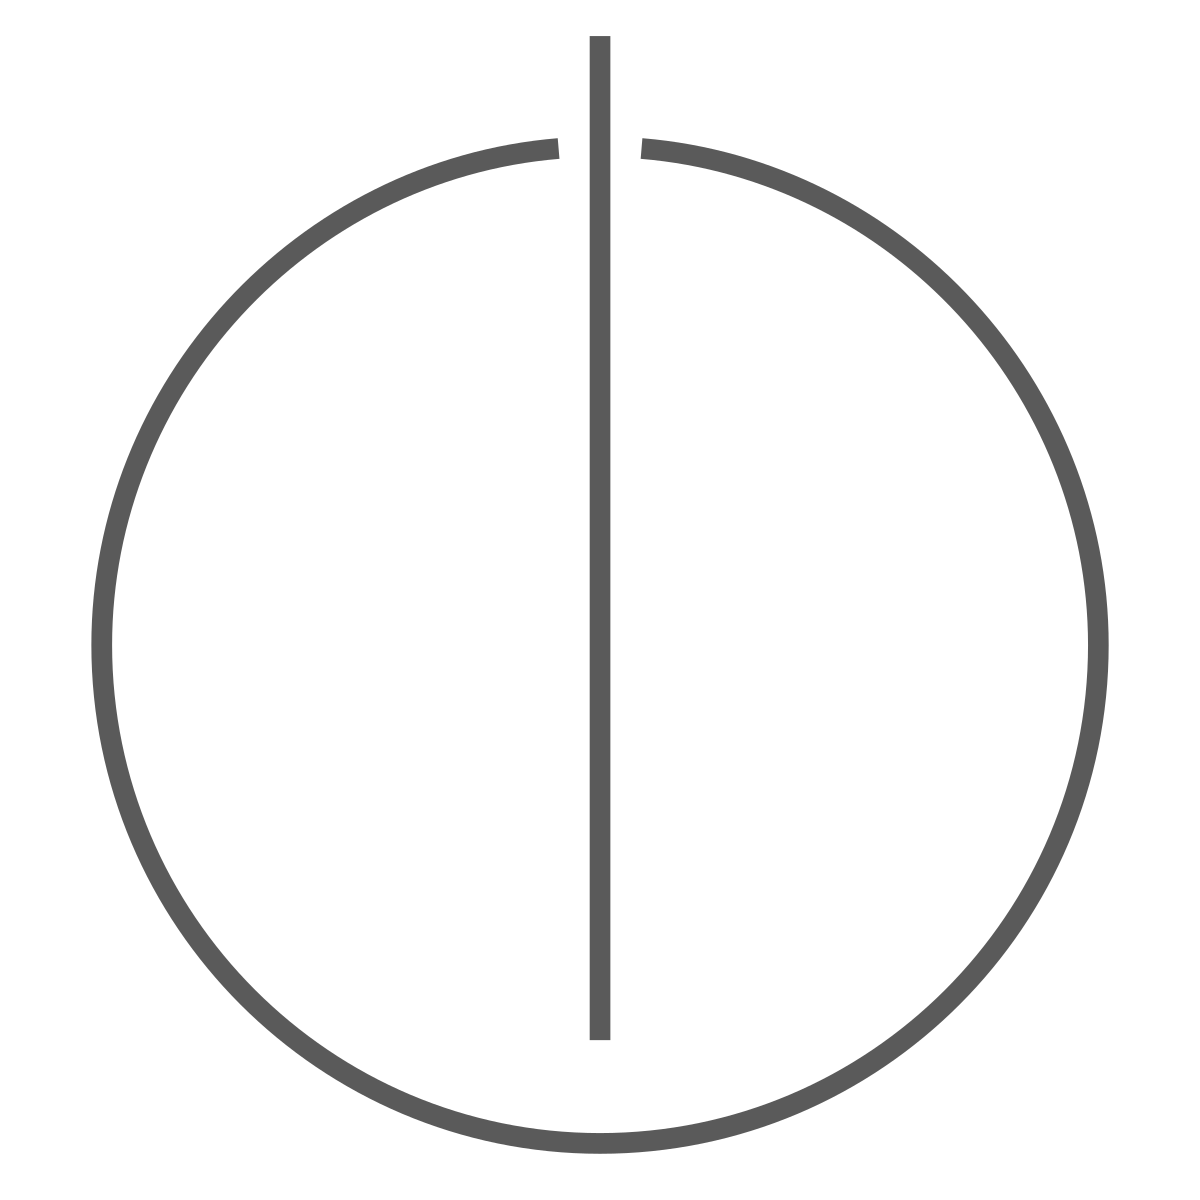
\includegraphics[height=20mm]{logos/tum_informatik_logo.png}
  }{}
\end{titlepage}


\frontmatter{}

\begin{titlepage}
  \centering

  \IfFileExists{logos/tum_logo.png}{%
    
\includegraphics[height=20mm]{logos/tum_logo.png}
  }{%
    \vspace*{20mm}
  }

  \vspace{5mm}
  {\huge\MakeUppercase{\getFaculty{}}}\\

  \vspace{5mm}
  {\large\MakeUppercase{\getUniversity{}}}\\

  \vspace{20mm}
  {\Large \getDoctype{}}

  \vspace{15mm}
  {\huge\bfseries \getTitle{} \par}

  \vspace{10mm}
  {\huge\bfseries \foreignlanguage{german}{\getTitleGer{}} \par}

  \vspace{15mm}
  \begin{tabular}{l l}
    Author:          & \getAuthor{} \\
    Supervisor:      & \getSupervisor{} \\
    Advisor:         & \getAdvisor{} \\
    Submission Date: & \getSubmissionDate{} \\
  \end{tabular}

  \IfFileExists{logos/tum_informatik_logo.png}{%
    \vfill{}
    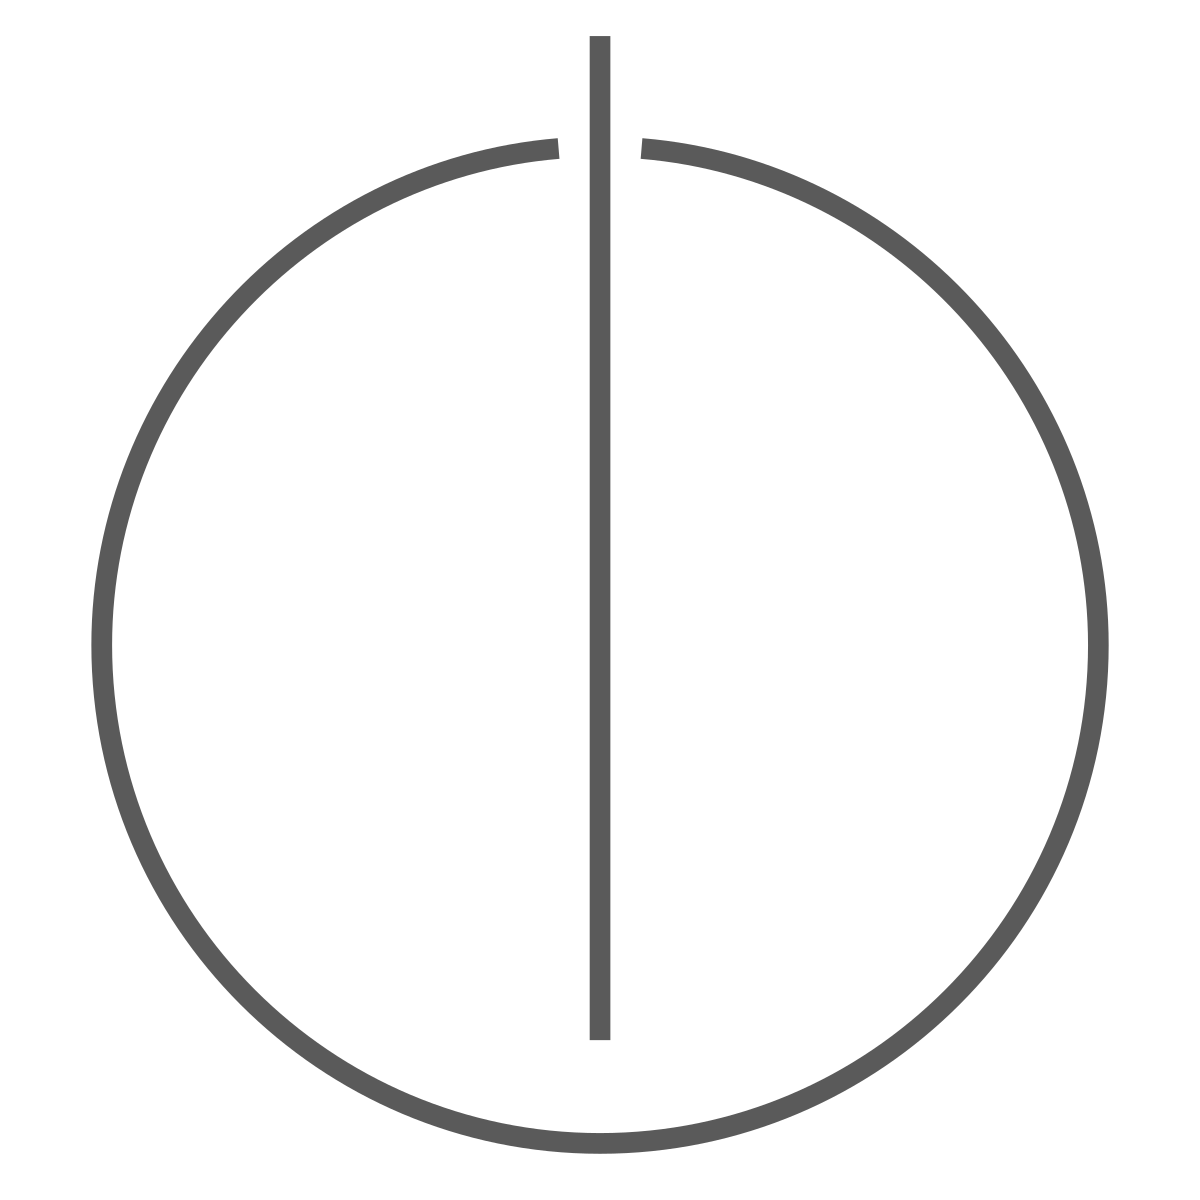
\includegraphics[height=20mm]{logos/tum_informatik_logo.png}
  }{}
\end{titlepage}

\thispagestyle{empty}
\vspace*{0.8\textheight}
\noindent
I confirm that this \MakeLowercase{\getDoctype{}} is my own work and I have documented all sources and material used.

\vspace{15mm}
\noindent
\getSubmissionLocation{}, \getSubmissionDate{} \hspace{50mm} \getAuthor{}

\cleardoublepage{}

\addcontentsline{toc}{chapter}{Acknowledgments}
\thispagestyle{empty}

\vspace*{20mm}

\begin{center}
{\usekomafont{section} Acknowledgments}
\end{center}

\vspace{10mm}

%TODO: Acknowledgments

\cleardoublepage{}

\chapter{\abstractname}

%TODO: Abstract

Fake news is becoming a more significant issue as mainstream news source becomes social media. Social media is capable of disseminating information at a rapid pace, which leads to widespread fake news in a matter of hours. The consequences of sharing misleading information can be destructive at many levels. This is why fake news, rumor, deception, and other aspects of false information are being studied to be automatically detected. Many studies focus on different aspects, creating a variety of perspectives for automated detection. However, this is not an easy and straightforward task. There exist many challenges considering fake news, from human psychology to language modeling. Humans are not good lie detectors and can easily be fooled by misdirections, untrustworthy sources, or social status. Therefore, we need systems that can tell the difference.\\
Nevertheless, languages have many features which need to be utilized efficiently by automated detection systems to distinguish real news from fake news. As we will discuss, even though news content is important, social context also proves to be essential in detecting fake news.\\
This thesis investigates two types of fake news detection models: a news content-based model and a model that utilizes both news content and social context called a mixed model or mixed approach.  These models were developed in other studies. We reproduce their work using their datasets and attempt to explain their models. We investigate the explainability of two kinds of neural networks, an inductive graph neural network and, a Transformer model. We explain the Transformer model with the partition explainer from the SHAP framework. The mixed model is explained by GNNExplainer, a recent and only study that attempts to explain the graph neural networks and provide the library for it. We report our findings as well as improvement suggestions for GNNExplainer.\\
From what we gathered from our experiments, we propose the adoption of input sensitivity analysis along with explanation techniques to discover unintended weaknesses of  the model. We also draw attention to the importance of interpretable and understandable explanations and suggest better visualization techniques where necessary.

\microtypesetup{protrusion=false}
\tableofcontents{}
\microtypesetup{protrusion=true}

\mainmatter{}

% !TeX root = ../main.tex
% Add the above to each chapter to make compiling the PDF easier in some editors.

\chapter{Introduction}\label{chapter:introduction}

With the rapid development of communication technologies, social media has become one of the most frequently used news sources. For example, a study from Pew Research Center\footnote{https://www.pewresearch.org/journalism/2021/09/20/news-consumption-across-social-media-in-2021/} reports that in 2021, 48\% of U.S. adults get their news from social media “often” or “sometimes”. As another example, global data from 2022\footnote{https://www.statista.com/statistics/718019/social-media-news-source/} shows that over 70\% of adults from Kenya, Malaysia, Phillippines, Bulgaria, and Greece use social media as one of their news sources, while this share is lower than 40\% for the adults in the United Kingdom, The Netherlands, Germany, and Japan. These statistics indicate that social media is a crucial news source. Still, one should follow the news on social media carefully since there is no regulatory authority to check the news. For instance, a study in Digital News Report 2022~\parencite{ReutersInstituteDigitalNewsReport}  reports in its key findings that trust in the news is 42\% globally, the highest (69\%) in Finland, and the lowest (26\%) in the U.S.A. Consequently, the same study shows in early 2022, in the week of the survey, between 45\% and 55\% of surveyed social media consumers worldwide have witnessed false or misleading information about COVID-19.

The term fake news has existed for over a century~\parencite{TheScienceOfFakeNews_Lazer}.  It rose to prominence with the 2016 U.S. Presidential Election~\parencite{USPresidentialElection2016}. With its prevalence, the research community has focused on the automatic detection of fake news~\parencite{FakeNewsDetectionOnSocialMedia_Shu, FakeNewsNet_Shu,  LiarLiarPantsOnFire, FakeNewsDetectionUsingGeometricDeepLearning, SupervisedLearningForFakeNewsDetection}.



\subsection{Subsection}

See~\autoref{tab:sample}, \autoref{fig:sample-drawing}, \autoref{fig:sample-plot}, \autoref{fig:sample-listing}.

\begin{table}[htpb]
  \caption[Example table]{An example for a simple table.}\label{tab:sample}
  \centering
  \begin{tabular}{l l l l}
    \toprule
    A & B & C & D \\
    \midrule
    1 & 2 & 1 & 2 \\
    2 & 3 & 2 & 3 \\
    \bottomrule
  \end{tabular}
\end{table}

\begin{figure}[htpb]
  \centering
  % This should probably go into a file in figures/
  \begin{tikzpicture}[node distance=3cm]
    \node (R0) {$R_1$};
    \node (R1) [right of=R0] {$R_2$};
    \node (R2) [below of=R1] {$R_4$};
    \node (R3) [below of=R0] {$R_3$};
    \node (R4) [right of=R1] {$R_5$};

    \path[every node]
    (R0) edge (R1)
    (R0) edge (R3)
    (R3) edge (R2)
    (R2) edge (R1)
    (R1) edge (R4);
  \end{tikzpicture}
  \caption[Example drawing]{An example for a simple drawing.}\label{fig:sample-drawing}
\end{figure}

\begin{figure}[htpb]
  \centering

  \pgfplotstableset{col sep=&, row sep=\\}
  % This should probably go into a file in data/
  \pgfplotstableread{
    a & b    \\
    1 & 1000 \\
    2 & 1500 \\
    3 & 1600 \\
  }\exampleA
  \pgfplotstableread{
    a & b    \\
    1 & 1200 \\
    2 & 800 \\
    3 & 1400 \\
  }\exampleB
  % This should probably go into a file in figures/
  \begin{tikzpicture}
    \begin{axis}[
        ymin=0,
        legend style={legend pos=south east},
        grid,
        thick,
        ylabel=Y,
        xlabel=X
      ]
      \addplot table[x=a, y=b]{\exampleA};
      \addlegendentry{Example A};
      \addplot table[x=a, y=b]{\exampleB};
      \addlegendentry{Example B};
    \end{axis}
  \end{tikzpicture}
  \caption[Example plot]{An example for a simple plot.}\label{fig:sample-plot}
\end{figure}

\begin{figure}[htpb]
  \centering
  \begin{tabular}{c}
    \begin{lstlisting}[language=SQL]
    SELECT * FROM tbl WHERE tbl.str = "str"
  \end{lstlisting}
  \end{tabular}
  \caption[Example listing]{An example for a source code listing.}\label{fig:sample-listing}
\end{figure}

% !TeX root = ../main.tex
% Add the above to each chapter to make compiling the PDF easier in some editors.

\chapter{Background and Related Work}\label{chapter:background}

We explain two research fields that create the bedrock of this thesis, namely, fake news detection and
explainable artificial intelligence. Both areas provide the foundation of tools used in this work. The first
provides the mechanisms and approaches to detect fake news, and the second offers a suite of techniques to interpret these mechanisms and strategies.\\
Initially, in \ref{sec:fakeNewsDetection}, we discuss societal challenges, the characteristics, and the history of fake news. Then we talk about the detection methods that were developed over the years. After showing the challenges of creating FND models, we conclude the first section with SOTA FND models.\\
After fake news detection, in \ref{sec:explainableArtificialIntelligence}, we first examine when XAI is necessary and its importance. Then, we define the suite of explainable artificial intelligence and the goals of XAI, and finally, we determine the suite that aims to satisfy these goals.\\
\section{Fake News Detection}
\label{sec:fakeNewsDetection}
In the past decade, social media has become a place where anyone can share information. Although fast, free, and easy to access, obtaining real news from social media can be difficult, and one should do so at their own risk and always check the facts~\parencite{SocialMediaAndFakeNewsIn2016Election_Allcott,TheScienceOfFakeNews_Lazer}. Nevertheless, the news stream never ends; thus, the need to verify the credibility of news using automated systems arises. To address this necessity, the number of studies involving \emph{Fake News} or \emph{Fake News Detection} has dramatically increased in the last decade (Fig. \ref{fig:FN_vs_FND_Publications}).
\begin{figure}
    \centering
    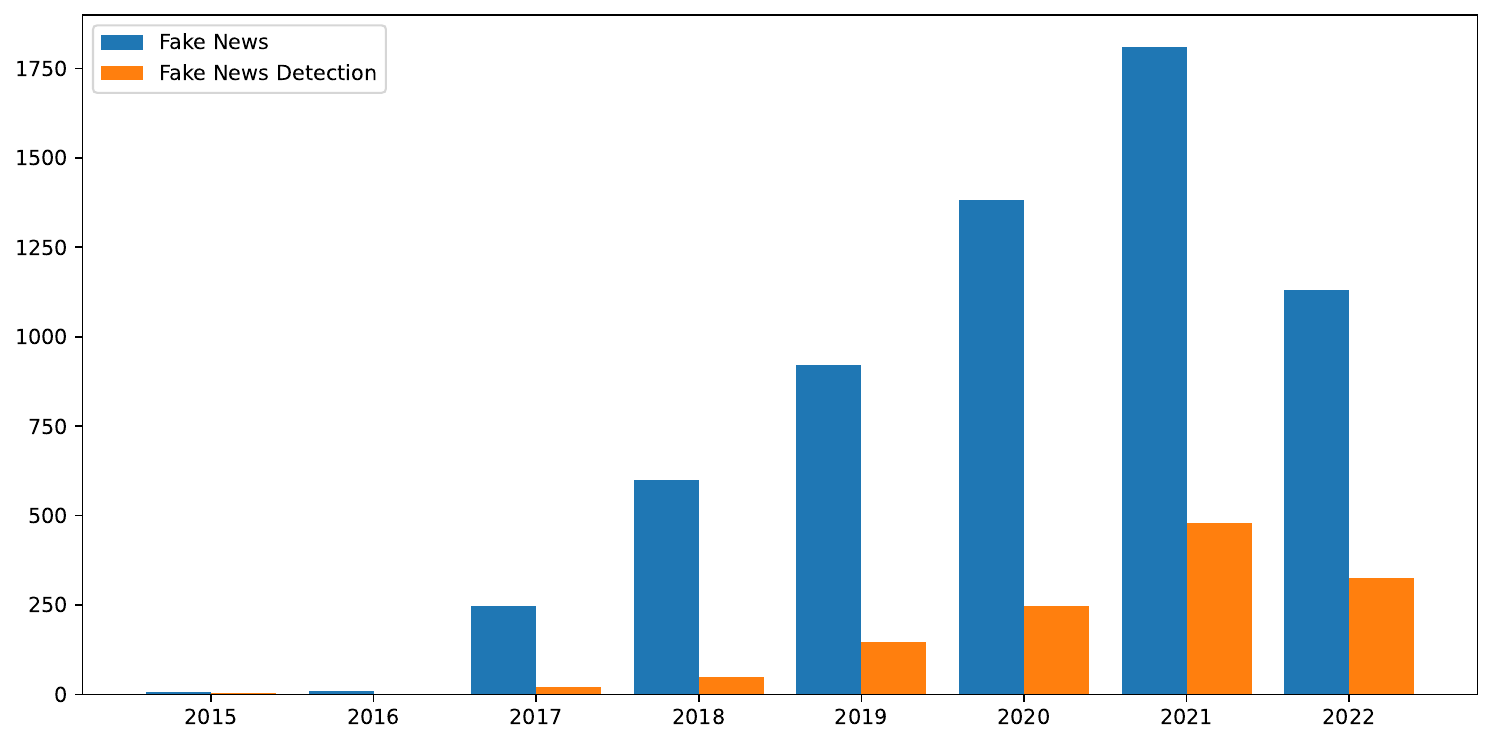
\includegraphics[scale=0.5]{FN_vs_FND_Publications}
    \caption[Fake News and Fake News Detection Publications by Year]{Total number of publications that include (1) \emph{Fake News} (blue) and (2) \emph{Fake News Detection} (orange) publications by year. Source: Scopus; Search Arguments: (1) TITLE-ABS-KEY("fake news*") PUBYEAR AFT 2014 (2) TITLE-ABS-KEY("fake news detection")}\label{fig:FN_vs_FND_Publications}
\end{figure}\\
In \ref{subsec:fakeNewsDetection_fakeNews}, we briefly present the history of fake news and look at studies that display the impact of fake news on society. In this section, we also define the terms fake news, disinformation, and misinformation. \\
In \ref{subsec:fakeNewsDetection_FoundationsOfFakeNews}, we make an excursion into social sciences and human psychology, delivering insights into why humans fall for or tend to believe fake news. Furthermore, we draw some insights from the social, technical, and data-oriented foundations of fake news.\\
We then list the available datasets used in FND and deliberate their advantages and disadvantages in \ref{subsec:fakeNewsDetection_Evolution}. Finally, in \ref{subsec:fakeNewsDetection_Evolution}, we summarize the evolution of detection algorithms, then we classify FND algorithms with respect to their input data type and what they focus on that data.

\subsection{Fake News}
\label{subsec:fakeNewsDetection_fakeNews}
Throughout history, various forms of widespread fake news have been recorded. For instance, in the thirteenth
century BC, Rameses the Great decorated his temples with paintings that tell stories of victory in the Battle
of Kadesh. However, the treaty between the two sides reveals that the battle's outcome was a
stalemate~\parencite{HistorysGreatestLies_Weir}. Just after the printing press was invented in 1439, the
circulation of fake news began. One of history's most famous examples of fake news is the
“Great Moon Hoax”~\parencite{TheGreatMoonHoax_Foster}. In 1835, The Sun newspaper of New York published articles about a real-life astronomer and a made-up colleague who had observed life on the moon. It turns out that these fictionalized articles brought them new customers and almost no backlash after the newspaper admitted that the articles mentioned earlier were a hoax\footnote{\url{https://www.politico.com/magazine/story/2016/12/fake-news-history-long-violent-214535/}}.\\
In order to highlight the difference, using the definitions from~\parencite{ThePsycologyOfFakeNews_Pennycook}, we formally introduce the terms disinformation and misinformation as follows.
\begin{definition}[\emph{Disinformation}]
    "\emph{Information that is false or inaccurate and was created with a deliberate intention to mislead people.}"~\parencite{ThePsycologyOfFakeNews_Pennycook}
\end{definition}
\begin{definition}[\emph{Misinformation}]
    "\emph{Information that is false, inaccurate, or misleading. Unlike disinformation, misinformation does not necessarily need to be created deliberately to mislead.}"~\parencite{ThePsycologyOfFakeNews_Pennycook}
\end{definition}
There is no fixed definition for fake news. Thus, we elaborate on the definitions of fake news. A limited definition is news articles that are intentionally or verifiably false~\parencite{SocialMediaAndFakeNewsIn2016Election_Allcott}. This definition stresses authenticity and intent. The inclusion of false information that can be confirmed refers to authenticity. On the other hand, intent refers to the deceitful intention to delude news consumers~\parencite{FakeNewsDetectionOnSocialMediaADataMiningPerspective_Shu}. This definition is widely used in other studies~\parencite{AutomaticDeceptionDetection_Conroy, TheFakeNewsSpreadingPlague_Mustafaraj, FakeNewsDetectionOnSocialMediaADataMiningPerspective_Shu}.\\
Furthermore, recent social sciences studies~\parencite{TheScienceOfFakeNews_Lazer, ThePsycologyOfFakeNews_Pennycook} define fake news as fabricated information that mimics news media content in form but not in organizational process or intent. Similarly, this definition covers authenticity and intent; additionally, it includes the organizational process. More general definitions for fake news consider satire news as fake news due to the inclusion of false information even though satire news aim to entertain and inherently reveals its deception to the consumer~\parencite{WhenFakeNewsBecomesReal_Balmas, TheImpactOfRealNewsAboutFakeNews_Brewer, NewsVerificationByExploitingConflictingSocialViewpoints_Jin, FakeNewsOrTruthUsingSatiricalCues_Rubin}. Further definitions include hoaxes, satires, and obvious
fabrications~\parencite{DeceptionDetectionForFakeNews3TypesOfFakeNews_Rubin}
In this thesis, we are not interested in the organizational process and do not consider conspiracy theories~\parencite{ConspiracyTheories_Sunstein}, superstitions~\parencite{Superstition_Lindeman}, rumors~\parencite{RumorsAndHealthCareReform_Berinsky}, misinformation, satire, or hoaxes. Therefore, we use the limited definition from~\parencite{SocialMediaAndFakeNewsIn2016Election_Allcott} and formally introduce it.
\begin{definition}[\emph{Fake News}]
    "\emph{News articles that are intentionally or verifiably false.}"~\parencite{SocialMediaAndFakeNewsIn2016Election_Allcott}
\end{definition}
Fake news can lead to disastrous situations, such as crashes in stock markets, resulting in millions of dollars. For example, Dow Jones
industrial average went down like a bullet (see Fig. \ref{fig:MarketReactionToFakeTweet}) after a tweet about an explosion injuring President Obama
went out due to a hack~\parencite{MarketQuaversAfterFakeAPTweet_ElBoghdady}.
\begin{figure}
    \centering
    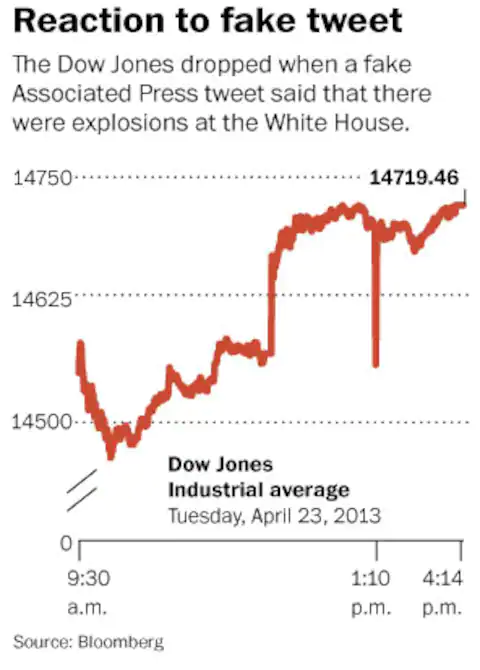
\includegraphics[scale=0.2]{MarketReactionToFakeTweet}
    \caption[Market Reaction to Fake Tweet]{The market's reaction to the fake tweet. The sharp decline caused by a single tweet. Image obtained from~\parencite{MarketQuaversAfterFakeAPTweet_ElBoghdady}}\label{fig:MarketReactionToFakeTweet}
\end{figure}\\
The detrimental impacts of fake news further extend to societal issues.
When fake news rose to prominence with the 2016 U.S. Presidential Election~\parencite{USPresidentialElection2016}, a man, convinced by what he
read on social media about a pizzeria trafficking humans, went on a shooting spree in that pizzeria. Later named
Pizzagate~\parencite{Pizzagate_Fisher}, this incident illustrates the deadly impact of fake news. In fact, fake news can even affect presidential elections~\parencite{SocialMediaAndFakeNewsIn2016Election_Allcott, TrumpWonBecauseOfFacebook_Read}.\\
Recent history exhibits that some fake news spreads like wildfires through social media. Evidence shows that the most popular fake news stories
were more widely shared than the most popular mainstream news stories~\parencite{Buzzfeed_FakeNewsOutperformRealNews_Silverman}.\\
Digital News Report 2022~\parencite{ReutersInstituteDigitalNewsReport} reports in its key findings that trust in the news is 42\% globally,
the highest (69\%) in Finland, and the lowest (26\%) in the U.S.A. Additionally, the same study shows that in early 2022, in the week of the
survey, between 45\% and 55\% of the surveyed social media consumers worldwide witnessed false or misleading information about COVID-19. The
same study also reports the appearance of fake news in politics was between 34\% and 51\%, and between 9\% and 48\% for fake news about
celebrities, global warming, and immigration~\parencite{StatistaUsageOfSocialMedia_Watson}.
\begin{figure}
    \centering
    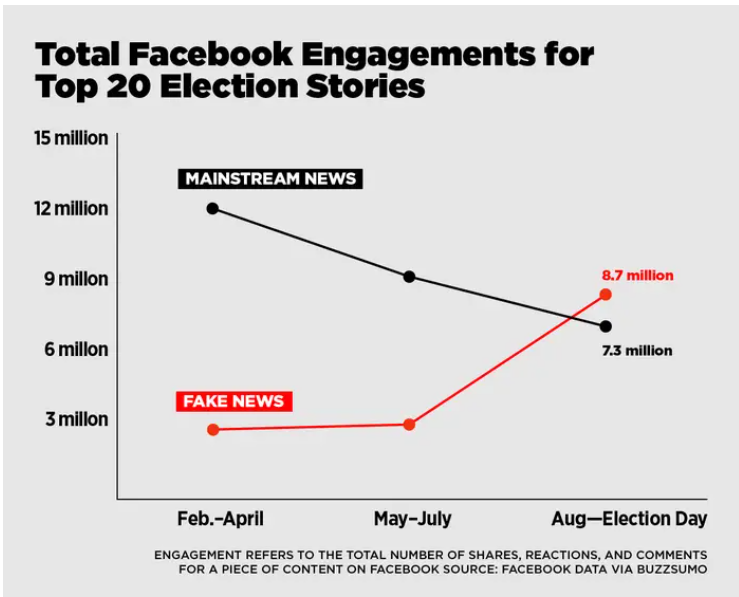
\includegraphics[scale=0.4]{TotalFacebookEngagementsForTop20ElectionStories}
    \caption[Total Facebook Engagements for Top 20 Election Stories]{The rising engagement for fake news stories observed after May-July, just before Presidential Elections. Image obtained from~\parencite{Buzzfeed_FakeNewsOutperformRealNews_Silverman}}\label{fig:TotalFacebookEngagementsForTop20ElectionStories}
\end{figure}
\subsection{Foundations of Fake News}
\label{subsec:fakeNewsDetection_FoundationsOfFakeNews}
The environment for fake news has been the traditional news media for a long time. First started with newsprint,
then continued with radio and television, and now with social media and the web, the dissemination of fake news reached its peak. Next, we discuss the psychological and social foundations of fake news to stress the importance
of human psychology, especially when accepting fake news as genuine and sharing it with others. Then we focus on
the technical foundations where we discuss how social media and technologiy have accelerated the diffusion of fake news.\\
\textbf{Psychological Foundations.}  Understanding the difference between real and fake news is not an easy task
for a human. Two psychological theories, namely, \emph{naive realism} and \emph{confirmation bias}, examine why humans fall for fake news. The first refers to a person's disposition to believe that their point of view is the
mere accurate one, while people who believe otherwise are uninformed or biased~\parencite{NaiveRealism_Reed}.
The second, often called selective exposure, is the proclivity to prefer information that confirms existing views~\parencite{ConfirmationBias_Nickerson}.\\
Another reason for human fallacy in fake news is that once a misperception is formed, it becomes difficult to correct. In fact, it turns out that correcting people leads them to believe false information more, especially
when given factual information that refutes their beliefs~\parencite{WhenCorrectionsFail_Nyhan}.\\
\textbf{Social Foundations.}  The prospect theory explains the human decision-making process as a mechanism
based on maximizing relative gains and minimizing losses with respect to the current
state~\parencite{ProspectTheory_Kahneman, AdvancesInProspectTheory_Kahneman}. This inherent inclination to get the highest reward also applies to social cases in which a person will seek social networks that provide them with
social acceptance. Consequently,  people with different views tend to form separate groups, which makes them feel safer, leading to the consumption and dissemination of information that agrees with their opinions. These behaviors are explained by social identity theory~\parencite{SocialIdentityTheory_Ashforth} and normative social influence~\parencite{NormativeSocialInfluence_Asch}.\\
Two psychological factors play a crucial role here~\parencite{TheRussianFirehoseOfFalsehood_Paul}. The first, social credibility, is explained by a person’s tendency to recognize a source as credible when that source is deemed credible by other people. The second, called the frequency heuristic, is the acceptance of a news piece by repetitively being exposed to it. Collectively, these psychological phenomena are closely related to the well-known filter bubble~\parencite{TheFilterBubble_Pariser}, also called echo chamber, which is the formation of homogenous bubbles in which the users are people of similar ideologies and share similar ideas. Being isolated from different views, these users usually are inclined to have highly polarized opinions~\parencite{EchoChambers_Sunstein}. As a result, the main reason for misinformation dispersal turned out to be the echo
chambers~\parencite{TheSpreadingOfMisinformationOnline_DelVicario}.\\
\textbf{Technical Foundations.} Social media's easy-to-use and connected nature give rise to more people selecting or even creating their own news source. Naturally, this gives way to more junk information echoing in a group of people on social media. As algorithms evolve to understand user preferences, social media platforms recommend similar people or groups to those in echo chambers. A recent study~\parencite{TheEffectOfPeopleRecommenderOnEchoChambers_Cinus}  shows that these recommenders can strengthen these echo chambers. They discuss that some of these recommenders contribute to the polarization on social media. In other words, people can convince themselves that any fake news is real by staying in their echo chambers. One main reason that some fake news spreads so rapidly on social media is the existence of malicious accounts. The account user can be an actual human or a social bot since creating accounts on social media is no cost and almost no effort. While many social bots provide valuable services, some were designed to harm, mislead, exploit, and manipulate social media discourse. Formally, a social bot is a social media account governed by an algorithm to fabricate content and interact with other users~\parencite{TheRiseOfSocialBots_Ferrara}. A more recent study from the same author shows that malicious social bots were heavily used in the 2016 U.S. Presidential Elections~\parencite{SocialBotsDistortThe2016USPresidentialElection_Bessi}. On the other hand, malicious accounts that are not bots, such as online trolls who aim to trigger negative emotions and humans that provoke people on social media to get an emotional response, contribute to the proliferation of fake news~\parencite{AnyoneCanBecomeATroll_Cheng}.\\
Building upon three foundations, we draw some results for fake news to be considered when building a fake news detection model:
\begin{enumerate}
    \item \emph{Invasive}: Fake news can appear on anyone’s feed if it spreads for a sufficient amount of time.
    \item \emph{Hard to discern}: Fake news is fabricated in such a way that it resembles the authenticity of a real news source. This
          indistinguishability leads to issues when working with news-content-based FND models.
    \item \emph{The source is crucial}: The credibility of a news source is essential. We can use news from credible sources to teach the model
          to distinguish genuine from fabricated.
    \item \emph{Fake news has hot spots}: The echo chambers are invaluable examples when trying to understand the behaviors of fake news. We can
          leverage this attribute and use social models, such as graphs, to successfully detect fake news.
    \item \emph{Early detection is essential}: As discussed in psychological foundations, the volume of exposure to a piece of fake news can significantly affect one’s opinions, thus leading to more misinformed individuals.
\end{enumerate}
\textbf{Data-Oriented Foundations.} We define features for news content and social context to represent the news pieces in a structured manner. First, we introduce attributes for news content~\parencite{FakeNewsDetectionOnSocialMediaADataMiningPerspective_Shu}:
\begin{itemize}
    \item \emph{Source}: Publisher of the news piece.
    \item \emph{Headline}: Short title text that aims to catch the readers’ attention and describes the article's main topic.
    \item \emph{Body Text}: The main text piece that details the news story.
    \item \emph{Image/Video}: Part of the body content supplies visual input to articulate the story.
\end{itemize}
Using these attributes, we extract two types of features for news content:
\begin{description}
    \item{\emph{Linguistic-based features}:} The news content is heavily based on textual content. Thus, the first feature that belongs to this class is lexical features which make use of character and word level frequency information which can be obtained by the utilization of
    \emph{term frequency}-\emph{inverse term frequency} (TF-IDF)~\parencite{TF_Luhn, IDF_Jones} or bag-of-words (BoW). The second feature is based on syntactic features which include sentence-level features that can be obtained via \emph{n-grams} and punctuation and \emph{parts-of-speech} (POS)~\parencite{POS_Daelemans} tagging. We can extend these features to domain-specific ones, such as external links and the number of graphs~\parencite{AStylometricInquiry_Potthast}.
    \item{\emph{Visual-based features}:} Particularly for fake news, the visual content is a strong tool for establishing
    belief~\parencite{VisualMisAndDisinformation_Viorela}. Hence, the features that reside in images and videos become significant. Fake images
    and videos which brings the fake story together are commonly used(e.g.~\cite{PutinBehindBars_Harding, DeepFakeQueensSpeech_Sawer}). To counteract the effects of misleading visual input, recent studies~\parencite{ExploitingMultiDomainVisualInformation_Qi} examined visual and statistical information for fake news detection. Visual features consist of clarity score, similarity distribution histogram, diversity score, and clustering score. Statistical features are listed
    as count, image ratio, multi-image ratio etc.~\parencite{FakeNewsDetectionOnSocialMediaADataMiningPerspective_Shu}.
\end{description}
Now, we define features for social context, which has recently drawn much attention from the research community~\parencite{BeyondNewsContents_Shu, HierarchicalPropagationNetworksForFND_Shu}. Overall, we will concern three aspects of social context data: user-based, post-based, and network-based features.
\begin{description}
    \item{\emph{User-based}:} As mentioned in the Technical Foundations part of this subsection, fake news has various ways of disseminating, such as via echo chambers, malicious accounts, or bots. Therefore, analyzing user-based information can prove useful. We distinguish user-based features at the group and individual levels~\parencite{FakeNewsDetectionOnSocialMediaADataMiningPerspective_Shu}. Individual levels are extracted to deduce the credibility of each user by utilizing, for example, the number of followers and followees, the number of tweets authored by a user, etc~\parencite{InformationCredibilityOnTwiter_Castillo}. On the other hand, group-level user-based features are the general characteristics of groups of users related to the news~\parencite{AutomaticDetectionOfRumor_Yang}. Parallel to the social identity theory and normative social influence idea, the assumption is the consumers of real and fake news tend to form different groups, which may lead to unique characteristics. Typical group-level features stem from individual-level features by obtaining the share of verified users, and the average number of followers and followees~\parencite{DetectRumorsUsingTimeSeries_Ma}.
    \item{\emph{Post-based}:} Analysis of reactions by users can prove helpful when determining whether a news piece is real or not. For example, if a news piece is getting doubtful comments, this can help determine the news piece’s credibility. As such, post-based features are based on inferring the integrity of a news piece from three levels. Namely, post-level, group-level, and temporal-level~\parencite{FakeNewsDetectionOnSocialMediaADataMiningPerspective_Shu}. Post-level features can be embedding values for each post or take forms as mentioned in linguistic-based features, e.g., n-grams, BoW, etc. For post-level features, we can also consider general approaches such as topic extraction (e.g., using latent Dirichlet allocation (LDA)~\parencite{LatentDirichletAllocation_Blei}), stance extraction, which provides information about users’ opinions (e.g., supports, opposes~\parencite{NewsVerificationByExploitingConflictingSocialViewpoints_Jin}), and finally credibility extraction, which deals with estimating the degree of trust for each post~\parencite{InformationCredibilityOnTwiter_Castillo}. Group-level post-based features collect feature values for all relevant posts and apply an operation to extract pooled information. When determining the credibility of news, group-level features proved to be helpful~\parencite{NewsVerificationByExploitingConflictingSocialViewpoints_Jin}. Temporal-level features deal with changes in post-level features over time. Typically, unsupervised learning methods such as Recurrent Neural Networks (RNN) are employed to capture the changes over time~\parencite{DetectingRumorsFromMicroblogs_Ma}.
    \item{\emph{Network-based}:} As discussed in the Technical Foundations part, fake news is likely to give rise to echo chambers, which leads to the idea of a network-based approach. When represented as networks, the propagation behavior of fake news can be analyzed further, and patterns can be discovered~\parencite{FakeNewsDetectionOnSocialMediaADataMiningPerspective_Shu}. In literature, various types of networks exist, the most common ones are stance networks, occurrence networks, and friendship networks. Stance networks are constructed upon stance detections which is a part of sentiment analysis and deal with determining a user’s viewpoint using text and social data~\parencite{StanceClassificationAttention_Du}. Using all users’ stances, a network is built in which the nodes are the tweets relevant to the news piece and the edges represent the similarity of stances between nodes~\parencite{NewsVerificationByExploitingConflictingSocialViewpoints_Jin, SomeLikeItHoaxDataset_Tacchini}. On the other hand, occurrence networks leverage the frequency of mentions or replies about the same news piece~\parencite{ProminentFeaturesOfRumorPropagation_Kwon}. Friendship networks are based on the follower/followee relationship of users who share posts connected to the news piece. Derived from friendship networks, in the form of one of the datasets we use in our experiments~\parencite{UPFD_Dataset_Shu}, diffusion networks are designed to track the course of the dissemination of news~\parencite{ProminentFeaturesOfRumorPropagation_Kwon}. Briefly, a diffusion network consists of nodes representing users and diffusion paths representing the relationship and interaction between users. In detail, a diffusion path between two users $u_i$ and $u_j$ exists if and only if $u_j$ follows $u_i$, and $u_j$ shares a post about a news piece that $u_i$ has already shared a post about~\parencite{FakeNewsDetectionOnSocialMediaADataMiningPerspective_Shu}. It has been shown that characterizing these networks is possible~\parencite{ProminentFeaturesOfRumorPropagation_Kwon}. Approaches for these networks have gained traction recently, especially with some SOTA GNNs, e.g.,~\parencite{FakeNewsDetectionUsingGeometricDeepLearning_Monti}.
\end{description}
To conclude this subsection, we have covered psychological, social, technical, and data-oriented foundations in this section. We established that,  from different aspects, there are various reasons for the dissemination of fake news. Accordingly, we consider these reasons when building FND systems. In the next section, we discuss FND approaches and how they have evolved. Moreover, we characterize FND models and talk about each type of approach.

\subsection{Evolution of Fake News Detection}
\label{subsec:fakeNewsDetection_Evolution}
Fake news detection is as old as fake news itself. Before social media became a hub for news consumers, fact-checkers, i.e., fake news
detectors, were only journalists and literate people. Following the source shift of the news from printed paper to online, then social
media, detection of fabricated news have become costly, cumbersome, and not as rewarding due to the endless stream of information and
decreasing trust in journalism. Automatic detection for news thus became a necessity in our world~\parencite{NewsInAnOnlineWorld_Chen}.\\
Similar to what we did in the Data-Oriented Foundations part of the previous subsection, we classify fake news detection models as
\emph{News Content Models} and  \emph{Social Context Models} (see \ref{fig:FakeNewsDetectionModelsClassification}) and start with News Content Models by following the classification principles in~\parencite{FakeNewsDetectionOnSocialMediaADataMiningPerspective_Shu}.\\
\begin{figure}
    \centering
    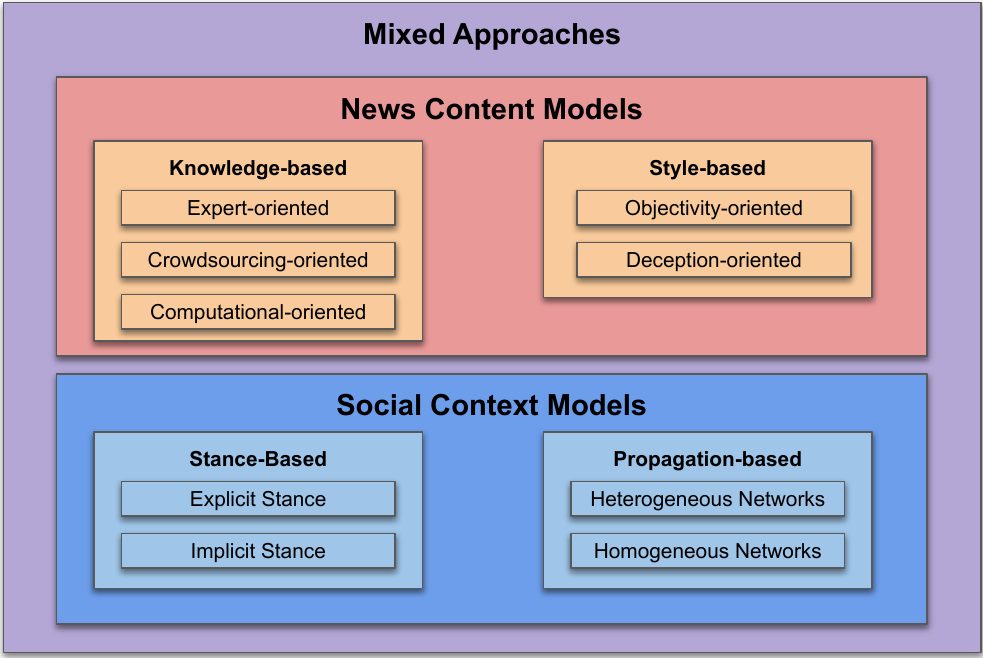
\includegraphics[scale=0.5]{FakeNewsDetectionModelsClassification}
    \caption[Characterization of Fake News Detection Models]{Characterization of Fake News Detection Models, Figure inspired by Figure 1 in~\cite{FakeNewsDetectionOnSocialMediaADataMiningPerspective_Shu}.}
    \label{fig:FakeNewsDetectionModelsClassification}
\end{figure}

\textbf{News Content Models.} Based on news content and fact-checking methodologies, these models are the starting point of fake news detection. News content models are classified as Knowledge-based and Style-based. We first introduce style-based models as they are the initial approaches for FND.
\begin{description}
    \item{\emph{Style-based}:} Previous research in psychology has mainly focused on style-based approaches to detect \emph{manipulators} in the text. Particularly deception detection techniques were popular and commonly developed in early works in criminology and psychology. We describe two different ways to approach style-based news content models, namely, \emph{Deception-oriented} and \emph{Objectivity-oriented}~\parencite{FakeNewsDetectionOnSocialMediaADataMiningPerspective_Shu}.
    \begin{itemize}
        \item \emph{Deception-oriented}: The initial approaches for automated fake news detection focus on news context and stem from deception detection in language. The first study that focuses deception detection in language~\parencite{DieEntwicklungDerGerichtspsychologischen_Undeutsch} hypothesized that the truthfulness of the statement is more important than the integrity of the reporting person, and there exist definable and descriptive criteria that form a crucial mechanism for the determination of the truthfulness of statements. Even though this study is from experimental psychology, it stresses the feasibility of defining a set of rules that determine the truthfulness of a statement.\\ An early study from criminology, Scientific Content Analysis (SCAN)~\parencite{SCAN_Sapir1987}, analyzes freely written statements.  In this process, SCAN claims to detect potential instances of deception in the text but cannot label a statement as a lie or truth. The next study for SCAN~\parencite{SCAN_Smith2001} is the first known study that correlates linguistic features with deceptive behavior using high-stakes data. Similar to SCAN, the subsequent studies  ~\parencite{CommunicationUnderStress_Adams, LyingWords_Newman} that link linguistic features to deception classify the owner of the statement as truth-teller or liar according to the frequency of deception indicators in the statement.\\Although for automated deception detection, defining a methodology is more challenging~\parencite{TheAccuracyConfidenceRelation_DePaulo}, early studies have shown that this task is achievable. A detailed study~\parencite{AutomatingLinguisticsBasedCues_Zhou} makes a structured approach using linguistic-based cues and draws attention to further studies for automating deception detection. In this study, the authors extend linguistic-based cues with complexity, expressivity, informality, and content diversity. Instead of using humans as cue identifiers, authors use \emph{Natural Language Processing} (NLP) techniques, namely an NLP tool called iSkim~\parencite{iSkim_Zhou}, to extract cues automatically. Another study also focuses on linguistic cue analysis. With a small dataset and employing the C4.5~\parencite{C45_Salzberg} algorithm, the authors reach 60.72\% accuracy using 15-fold cross-validation.\\Similarly, in ~\parencite{VerificatoinAndImplementationofLBDeceptionIndicators_Bachenko}, the authors developed a system for automatically identifying 275 truthful or deceitful statements with the use of verbal cues using Classification and Regression Tree (CART)~\parencite{ClassificationRegressioniTrees_Breiman}. Additionally, the studies ~\parencite{OnLyingAndBeingLiedTo_Hancock, OnDeceptionAndDeceptionDetection_Rubin} make use of a relatively small dataset and analyze linguistic-based cues. Rubin’s series of  studies~\parencite{OnDeceptionAndDeceptionDetection_Rubin, IdentificationOfTruth_Rubin, TruthAndDeception_Rubin, TowardsNewsVerification_Rubin} makes use of Rhetorical Structure Theory (RST) and Vector Space Modeling (VSM). The first captures the coherence of a story using functional relations among meaningful text units and delivers a hierarchical structure for each news story~\parencite{RST_William}. The second is the way to represent rhetorical relations in high-dimensional space. The authors utilized logistic regression as their classifier and reached 63\% accuracy.\\Furthermore, a study from Afroz and colleagues~\parencite{DetectingHoaxesFraudsAndDeception_Afroz} investigates stylistic deception and uses lexical, syntactic, and content-specific features. Lexical features include both character- and word-based features. Syntactic features represent sentence-level style and include frequency of function words from LIWC~\parencite{LIWC2007_Pennebaker}, punctuation, and POS tagging in which a text is assigned its morphosyntactic category~\parencite{POS_Daelemans}. Finally, content-specific features are keywords for a specific topic. For classification, the authors then leveraged Support Vector Machines (SVM)~\parencite{SVM_Hearst}. More comprehensive and modern approaches such as~\parencite{LiarLiarPantsOnFire_Wang} also leveraged the power of \emph{Convolutional Neural Networks} (CNNs) to determine the veracity of news.
        \item \emph{Objectivity-oriented}: Objectivity-oriented news content models aim to detect indicators of the lessening of objectivity in news content~\parencite{FakeNewsDetectionOnSocialMediaADataMiningPerspective_Shu}. These indicators are observed in the news from misleading sources, such as hyperpartisan sources which display highly polarized opinions in favor of or against a particular political party. Consequently, this polarized behavior motivates the fabrication of news that supports the sources’ political views or undermines the opposing political party. \emph{Hyperpartisan news} are a subtle form of fake news and  defined as misleading coverage of events that did actually occur with a strong partisan bias~\parencite{FightingMisinformationOnSocialMedia_Pennycook}. Since the spread of hyperpartisan news can be detrimental, many approaches to detect hyperpartisanship in news articles have been developed. For instance, in~\parencite{AStylometricInquiry_Potthast}, the authors take a stylometric methodology to detect hyperpartisan news. In this study, the authors employ 10 readability scores, and dictionary features where each feature represent the frequency of words from a carefully crafted dictionary in a given document with the help of General Inquirer Dictionaries~\parencite{TheGeneralInquirer_Stone}. A competition for detecting hyperpartisan news~\parencite{SemEvalHyperpartisanNewsDetection_Kiesel} hosted several teams with a variety of ideas which include the utilization of n-grams, word embeddings, stylometry, sentiment analysis etc. The most popular method was the usage of embeddings, particularly the models that leveraged BERT~\parencite{BERT_Devlin}.\\ Also used for dissemination of hyperpartisan news~\parencite{SemEvalHyperpartisanNewsDetection_Kiesel}, another form of fake news that is evaluated under this focus is \emph{Yellow-journalism}, which utilizes clickbaits such as catchy headlines, images etc. that invokes strong emotions, and it aims to generate revenue~\parencite{ClickbaitDetectionUsingDL_Agrawal, ClickbaitAndTabloidStrategies_Dolors}. Studies that aim to detect clickbaits mainly focus on headlines. For example, in~\parencite{DivingDeepIntoClickbaits_Rony}, the authors construct a DNN in which they use distributed subword embeddings~\parencite{EnrichingWordVectorsWithSubwordInfo_Bojanowski, BagOfTricksForTextClassificatoin_Joulin} as features with an extension of skip-gram model~\parencite{DistributedRepresentationsOfWords_Mikolov}.
    \end{itemize}
    \item{\emph{Knowledge-based}}: Being the most direct way of detecting fake news, these approaches make use of external fact-checkers to verify the claims in news content~\parencite{FakeNewsDetectionOnSocialMediaADataMiningPerspective_Shu}. Fact-checkers are either sophisticated algorithms, domain experts or crowdsourced to assess the truthfulness of a claim in a specific context~\parencite{FactChecking_Vlachos}. With growing attention on fake news detection, automated fact-checking has drawn much attention, and considerable efforts have been made in this area~\parencite{AutomatedFactChecking_Thorne, OverviewOfCheckThat_Barroncede}. We categorize knowledge-based news content models as \emph{Expert-oriented}, \emph{Crowdsourcing-oriented}, and \emph{Computational-oriented}.
    \begin{itemize}
        \item \emph{Expert-oriented}: These approaches are essentially dependent on human domain experts who investigate the integrity of a news piece collecting relevant information and documents to come up with a decision about the truthfulness of a claim~\footnote{\url{https://www.politifact.com/article/2018/feb/12/principles-truth-o-meter-politifacts-methodology-i/}}. Platforms like Politifact~\footnote{\url{https://www.politifact.com/}} and EUfactcheck~\footnote{\url{https://eufactcheck.eu/}} are examples for expert-oriented fact-checking for all news from a variety of sources. These platforms label news in a range such that the label reflects the veracity of the news. A different approach for labeling is exercised by Snopes~\footnote{\url{https://www.snopes.com/}}, which extends the same logic of Politifact by including different aspects of fact-checking such as Scam, Miscaptioned, Outdated, etc~\footnote{\url{https://www.snopes.com/fact-check-ratings/}}. Recently replaced by an irrelevant magazine website, another instance was Gossipcop~\footnote{\url{https://web.archive.org/web/20190807002653/https://www.gossipcop.com/about/}}, which dealt with celebrity fact-checking and contributed to the creation of fake news dataset~\parencite{FakeNewsNet_Shu}. Even though expert-based fact-checking is reliable, with the increasing magnitude of news stream and speed of spread, it is not scalable to fact-check every news piece by hand; thus, manual validation alone becomes insufficient~\parencite{ASurveyOnAutomatedFactChecking_Guo}.
        \item \emph{Crowdsourcing-oriented}: Powered by the wisdom of crowds~\parencite{WisdomOfCrowds_Galton}, crowdsourcing-oriented fact-checking is a collection of annotations that are afterward aggregated to obtain an overall result indicating the veracity of the news. Unlike professional fact-checkers, who are in short supply, this approach is scalable given that the crowd contains enough literate people~\parencite{ScalingUpFactChecking_Allen}.  For instance, Twitter launched a program called Birdwatch~\footnote{\url{https://twitter.github.io/birdwatch/overview/}}, in which the users are able to leave notes for tweets that they think contain misinformation. Furthermore, this tool allows users to rate each other’s notes, leading to the diversity of perspectives~\footnote{\url{https://twitter.github.io/birdwatch/diversity-of-perspectives/}}. Another example is from Facebook~\footnote{\url{https://www.facebook.com/formedia/blog/third-party-fact-checking-how-it-works}}, which uses a third party of crowdsourced fact-checkers called International Fact-Checking Network~\footnote{\url{https://www.poynter.org/ifcn/}} (IFCN).
        \item \emph{Computational-oriented}: Heavily dependent on external sources, computational-oriented models are scalable, automated systems that are designed to predict whether a claim is truthful or not. The studies that focus on this type of approach mainly try to solve two issues: (i) identifying check-worthy claims and (ii) estimating the integrity of claims~\parencite{FakeNewsDetectionOnSocialMediaADataMiningPerspective_Shu}. The first issue requires the extraction of factual claims from news content or other related textual content. For example, in~\parencite{DetectingCheckWorthyClaims_Hassan}, the authors collect presidential debate transcripts, then label them into three classes with the help of crowdsourcing. Using annotated data and supervised learning techniques, the authors uncover some interesting patterns in these transcripts. Another study that covers both issues uses Wikipedia information to generate factual claims and then check whether a given claim is truthful or not~\parencite{FEVER_Thorne}.  The second issue, compared to the first one, requires the utilization of structured external sources. \emph{Open web} and structured \emph{knowledge graphs} are the two most prominent tools when tackling this issue. Open web tools analyze features like mutual information statistics~\parencite{UnsupervisedNamedEntityExtraction_Etzioni}, frequency, and web-based statistics~\parencite{WebBasedStatisticalFactChecking_Magdy}.  On the other hand, knowledge graphs are interconnected. One noteworthy example is ontologies such as DBPedia~\parencite{DBPedia_Auer}, using which one can define semantic relations and rules in order to infer whether a claim is correct~\parencite{SemanticFakeNewsDetection_Bracsoveanu}.
    \end{itemize}
\end{description}

\textbf{Social Context Models.} The interconnected design of social media can be leveraged by extracting user-based, post-based, and network-based features and utilizing these features to supplement news content models. Social context models exploit related user engagements for a news piece by capturing this external information from multiple angles. Two types of social context models are prominent: \emph{Stance-based} and \emph{Propagation-based}~\parencite{FakeNewsDetectionOnSocialMediaADataMiningPerspective_Shu}.
\begin{itemize}
    \item \emph{Stance-based}: Given a news piece, these approaches estimate the user’s stance toward a specific news topic. More
          formally, stance detection in social media deals with users’ viewpoints toward particular topics by means of various aspects related
          to users’ posts and characteristic traits~\parencite{StanceDetectionOnSocialMeda_Abeer}. The user’s stance information can be
          extracted either implicitly or explicitly. Implicit stance can be automatically obtained from social media posts with the help of NLP
          tools such as sentiment analysis~\parencite{StanceAndSentimentINTweets_Saif}. Explicit stances are rather easier to obtain since they
          are direct expressions of opinions or emotions. For example, “like” on Twitter or Facebook, “upvote” and “downvote” ratings on Reddit,
          and “like” and “dislike” on Youtube are explicit stances of users. A study that utilizes explicit stances called Some Like it
          Hoax, uses logistic regression and harmonic boolean label crowdsourcing for classification on a dataset they curated from Facebook.
          In the stance classification process, they consider the likes and the issuer of likes for each post. They state that logistic regression comes short in this task since it cannot learn anything about posts without likes~\parencite{SomeLikeItHoaxDataset_Tacchini}. An early example of implicit stance detection leverages the dialogic relations between authors
          by constructing graphs that represent the interaction between authors. They show that this information can improve the performance
          of stance-detection models~\parencite{StanceClassificationDialogicProps_Walker}. A more detailed
          study~\parencite{StanceClassificationOnTwitterDebates_Addawood} investigates stance classification considering lexical,
          syntactic, twitter-specific and argumentation feature types. Although some twitter-specific features can be considered as explicit stances, such as if the tweet is a retweet, if a tweet contains the title to an article, if a tweet contains a hashtag, etc., those
          features are later aggregated before it is fed to the classifier. The authors reach the highest F1 score using lexical and argumentation features. In literature, there are also implicit stance-based approaches that aim to detect the veracity of a news
          piece by exploring the relationship between a headline and the article~\parencite{ARetrospectiveAnalysisOfFNC_Hanselowski, StanceDetectionInFakeNews_Ghanem}.\\Another variation of stance-based detection is rumor detection. One example of a rumor detection model is a Bayes classifier that utilizes content-based, network-based, and twitter-specific meme features through \emph{Information Retrieval} (IR) techniques~\parencite{RumorHasIt_Qazvinian}.  In this study, the authors propose a general framework that leverages statistical models and maximizes a linear function of log-likelihood ratios to retrieve rumorous tweets. They show that the features they used contribute to their model's overall performance.
    \item  \emph{Propagation-based}: Inspired by the assumption that the veracity of a news event is highly correlated with the credibilities of related social media posts, propagation-based models employ the interrelations of related social media posts to classify a news piece as truthful or not~\parencite{FakeNewsDetectionOnSocialMediaADataMiningPerspective_Shu}. These models can be based on either \emph{homogeneous networks} or \emph{heterogeneous networks}.
          Homogeneous networks are built upon a single type of entity, such as a post or
          event~\parencite{NewsVerificationByExploitingConflictingSocialViewpoints_Jin}. A study
          by~\cite{NewsVerificationByExploitingConflictingSocialViewpoints_Jin} created homogeneous credibility networks for each topic which
          is extracted using an unbalanced version of the Joint Topic Viewpoint
          Model~\parencite{FindingAndArguingExpressions_Trabelsi}. These credibility networks consist of nodes as tweets and edges as links, defined by either supporting or opposing. On the other
          hand, heterogeneous networks can contain multiple types of entities such as events, sub-events, posts, comments, etc. For example, in~\parencite{NewsCredibilityEvaluationOnMicroblog_Jin}, the authors build a hierarchical propagation graph that contains events, sub-events, and messages from parent to child, respectively. Using an iterative method, they provide a globally optimal solution for the graph optimization problem in the study.\\Furthermore, an interesting study from a decade ago based its credibility estimation
          algorithm on PageRank and similarity scores. Their propagation network consists of graphs in which possible nodes are events, tweets that were posted about that event, and users who posted those tweets.
\end{itemize}
\textbf{Mixed Approaches.} We examined two types of FND models, namely,  news content models and social context approaches. It is crucial to note that approaches are not necessarily purely news content or social context-based; they can be based on both. The models that use news content and social context are referred to as mixed approaches~\parencite{GraphNeuralNetworksWithContinualLearningFakeNewsDetection_Han}. \emph{User Preference-Aware Fake News Dataset} (UPFD)~\parencite{UPFD_Dataset_Shu} is a dataset that houses two of these types. The authors use news content and social engagement information to construct a hierarchical tree. The node features are textual representations of variety of sources which will be discussed in~\ref{sec:mixedApproaches}. The best-performing model uses GraphSAGE~\parencite{GraphSAGE_Hamilton} as graph encoder and BERT~\parencite{BERT_Devlin} as the text encoder and reaches 84.62\% and 97.23\% accuracy on Politifact and Gossipcop, respectively.\\
To summarize this section, we have introduced the history and definitions of fake news in subsection~\ref{subsec:fakeNewsDetection_fakeNews}. Then, we investigated the foundations of fake news and gave motivations for developing automated FND systems in subsection~\ref{subsec:fakeNewsDetection_FoundationsOfFakeNews}. Following that, we examined the evolution and characterized FND models in section~\ref{subsec:fakeNewsDetection_Evolution}. We have included at least two examples for each type of model and briefly summarized their approaches. We also briefly examined one of the datasets~\parencite{UPFD_Dataset_Shu} and models~\parencite{GraphSAGE_Hamilton} used in this thesis; however, in-depth information will be provided in the next chapter.\\
In~\ref{sec:explainableArtificialIntelligence}, we elaborate on the techniques available in explainable artificial intelligence. We discuss the qualities of a reasonable explanation, and we highlight the importance of the interpretability of a model. We give essential definitions that will be used throughout this thesis.

\section{Explainable Artificial Intelligence}
\label{sec:explainableArtificialIntelligence}
Understanding and interpreting a model's prediction is very important nowadays since this understanding allows to validate the reasoning of the model and extract rich information for a human expert, and can lead to increased trust in the model~\parencite{WhyShouldITrustYou_Riberio}. Furthermore, explanation of a model can help to improve the model~\parencite{AUnifiedApproach_Lundberg} and alleviate concerns raised by Ethical AI~\parencite{MachineBias_Angwin, EURegulationsOnDecisionMaking_Goodman}.
In this section, we introduce the background for XAI techniques that were used in this thesis. First, in~\ref{subsec:explainableArtificialIntelligence_Foundations} we characterize XAI by following works from~\cite{TheMythosOfModelInterpretability_Lipton} and~\cite{XAIConceptsTaxonomies_Arrieta} and give definitions to clarify the taxonomy. Then, in~\ref{subsec:explainableArtificialIntelligence_AGoodExplanation}, we discuss the properties of good explanations, the goals of XAI and the evaluation techniques for explanation ethods. Finally, in~\ref{subsec:explainableArtificialIntelligence_Overview} we briefly lay out the most frequently mentioned explanation methods in the literature, along with the ones we use in this thesis. We summarize each of them and cover explanation techniques offered to any kind of neural network.

\subsection{Foundations of Explainable Artificial Intelligence}
\label{subsec:explainableArtificialIntelligence_Foundations}
Initial AI methods were not sophisticated enough to require additional explanation schemes. In the last years, expanding applications of DNNs have led to the adoption of these opaque systems even more. Although empirically successful thanks to enormous parameter spaces and numerous layers, DNNs are complex \emph{black-box} models in terms of  interpretability~\parencite{CanWeOpenTheBlackBoxOfAI_Castelvecchi}.\\
In the XAI context, \emph{black-box} or \emph{opaque} models are considered to be the opposite of \emph{transparent} because they require a further search to understand their inner workings~\parencite{TheMythosOfModelInterpretability_Lipton}. Accordingly, humans hesitate to use
systems that are not directly interpretable and reliable~\parencite{xAIForDesigners_Zhu}, making \emph{interpretability} essential. Moreover, from a legal perspective, the notion \emph{right to explanation} brings more attention to interpretabilty~\parencite{TheMythosOfModelInterpretability_Lipton}. Particularly in situations such as when:
\begin{itemize}
    \item The prediction of AI directly affects human life, e.g., fully autonomous cars in traffic, medical AI assistants etc.
    \item The reasons behind an AI system’s decision can not be clearly determined.
\end{itemize}
With the additional demand from the Ethical AI field~\parencite{EURegulationsOnDecisionMaking_Goodman}, the research community has put in a great amount of effort to gap the bridge between a black-box model and its interpretability. However, the lack of consensus on taxonomy has led to synonymous usages of interpretability. The early definitions for interpretability were too broad, describing it as essentially an additional design driver when building a model~\parencite{TheBayesianCaseModel_Kim} or a requirement for \emph{trust}~\parencite{InteractiveAndInterpretableMLModels_Kim}. But can trust be defined in an objective way? Is the accuracy or F1 score of the model is enough to trust a model? To answer the first question, \cite{TheMythosOfModelInterpretability_Lipton} argues that trust is subjective and it is not technically defined. To answer the second question, taking only the performance metrics as a baseline for trust in the model is shown to be an incorrect approach, particularly studies that analyze models with \emph{adversarial examples}~\parencite{DetectingAdversarilaImageExamples_Bin, AdversarialExamples_Yuan}. Moreover, ~\cite{TowardsARigorousScienceML_Velez} argues that the need for interpretability comes from the \emph{incompleteness} of the problem formalization.\\
Instead of trying to find a technical definition for interpretability, we can categorize existing systems in terms of their transparency.
\cite{TheMythosOfModelInterpretability_Lipton} states two properties for interpretable models: \emph{transparency} and \emph{post-hoc interpretability}. The definition for the first and its related terms are given as in the following,
\begin{definition}[\emph{Understandability}]
    “\emph{Denotes the characteristic of a model to make a human understand its function - how the model works - without any need for explaining its internal structure or the algorithmic means by which the model processes data internally}”~\parencite{MethodsForInterpretingAndUnderstandingDNNs_Montavon,XAIConceptsTaxonomies_Arrieta}.
\end{definition}
\begin{definition}[\emph{Transparency}]
    “\emph{A model is considered to be transparent if by itself it is understandable}”~\parencite{XAIConceptsTaxonomies_Arrieta}.
\end{definition}
To elaborate further, we discuss degrees of transparent models as not all models provide the same extent of understandability~\parencite{XAIConceptsTaxonomies_Arrieta}. Both in~\cite{TheMythosOfModelInterpretability_Lipton} and \cite{XAIConceptsTaxonomies_Arrieta} the
categorization is made as: \emph{simulability}, \emph{decomposability}, and \emph{algorithmic transparency}. We discuss each of them briefly.
\begin{itemize}
    \item \emph{Simulability}: Denotes the model’s characteristic to be simulated or thought only by a human. Thus, the complexity of a model
          plays an important role here. Models that can be presented to a human in terms of text and visualizations are considered
          interpretable~\parencite{WhyShouldITrustYou_Riberio}, and in this case, models this elementary fall into simulatable models
          category~\parencite{XAIConceptsTaxonomies_Arrieta, RegressionShrinkage_Tibshirani}.
    \item \emph{Decomposability}: Represents the model’s characteristic to explain each part of the model. Basically, when all components of a model
          are simulable, then that model is decomposable~\parencite{TheMythosOfModelInterpretability_Lipton} given that the inputs are already interpretable~\parencite{XAIConceptsTaxonomies_Arrieta}.
    \item \emph{Algorithmic Transparency}: Deals with the user’s comprehension of the input’s journey from entering the model to becoming a prediction~\parencite{TheMythosOfModelInterpretability_Lipton, XAIConceptsTaxonomies_Arrieta}. For example, linear models can be considered algorihtmically transparent since the user can understand how the model can act in a given situation~\parencite{AnIntroductionToStatisticalLearning_Gareth}.
\end{itemize}
The second property of interpretable models, \emph{post-hoc explainability}, aims to improve the interpretability of not readily interpretable models. It does so by means of \emph{text explanations}, \emph{visual explanations}, \emph{local explanations}, \emph{explanations by example},
\emph{explanations by simplification}, and \emph{feature relevance explanations} techniques~\parencite{TheMythosOfModelInterpretability_Lipton, XAIConceptsTaxonomies_Arrieta}. In a more general sense, post-hoc explainability methods can be grouped into three categories in terms of the knowledge of the target model, granularity of focus, and form: \emph{model-specific or model-agnostic}, \emph{local or global} and \emph{form}. The first category refers to the explainability method's assumption on the model's structure. \emph{Model-specific} techniques can be utilized with a limited set of models since these techniques make an assumption on the model to be explained. On the other hand, \emph{model-agnostic} techniques are designed in such a way that does not require knowledge about model's inner workings~\parencite{XAIConceptsTaxonomies_Arrieta,ASurveyOfMethodsForExplainingBlackBoxModels_Guidotti}. The second category denotes the explanation's domain. \emph{Local} explanations reason about a particular prediction of a model at feature level~\parencite{TowardsARigorousScienceML_Velez} (e.g. compute a saliency map by taking the gradient of the output with respect to a given input vector~\parencite{TheMythosOfModelInterpretability_Lipton}), whereas global explanations aim to outline the model's general behavior on the dataset~\parencite{XAIConceptsTaxonomies_Arrieta, ASurveyOfMethodsForExplainingBlackBoxModels_Guidotti,TowardsARigorousScienceML_Velez}. Global explanations are usually presented in the structure of a series of rules~\parencite{InterpretableDecisionSets_Lakkaraju}. The third and last category, form of the explanation is the manner that is conveyed to the user. We will discuss specific forms of explanation in detail after we give a definition of \emph{explainability}, since from now on we talk about the explainability of a model rather than its interpretability.
\begin{definition}[Explainability]
    “\emph{Explainability is associated with the notion of explanation as an interface between humans and a decision maker that is, at the same time, both an accurate proxy of the decision maker and comprehensible to humans.}”~\parencite{XAIConceptsTaxonomies_Arrieta, ASurveyOfMethodsForExplainingBlackBoxModels_Guidotti}
\end{definition}
\begin{itemize}
    \item \emph{Text explanations} are techniques that learn to produce textual expressions that assist user to understand the outcomes of the model~\parencite{TowardsExplainableNeuralSymbolic_Bennetot}.
    \item \emph{Visual explanations} are techniques that supplement a model's explainability by visualizing the model's behavior. Due to the mismatch between high-dimensional nature of  complex ML systems and the capacity of human reasoning~\parencite{HowTheMachineThinks_Burrell}, visual explanations often employ dimensionality reduction practices~\parencite{XAIConceptsTaxonomies_Arrieta}.
\end{itemize}
From the perspective of explainability, one would intuitively prefer transparency since transparent models
can be explained with ease. However, some works argue that as transparency of a model increases their performance usually tends to decrease~\parencite{ExplaniableAIASurvey_Dosilovic}, although other works argue that this is not necessarily true, particularly in cases where the data is well structured and the quailty and value of available features is outstanding~\parencite{StopExplainingBlackBoxmodels_Rudin}. Furthermore, considering FND models, the
need for big and complex models can not be avoided since news pieces tend to be long texts, or social networks are represented as graphs, thus forcing SOTA FND models to utilize complex approaches that decreases transparecy such as word embeddings, data fusion, graph data structure~\parencite{UPFD_Dataset_Shu}.\\
On the other hand, although global explanations can be helpful to domain experts by providing information about what model has learnt on a global level, it might be difficult to obtain~\parencite{TheMythosOfModelInterpretability_Lipton}. Instead, local explanation methods are more easier to obtain and more practical for real-world applications. For example, if a user requests an explanation for a prediction, local explanations can provide it, which also complies with "right to explanation"~\parencite{EURegulationsOnDecisionMaking_Goodman}.\\
Depending on the model adopted for FND, we might be required to use model-specific or model-agnostic approaches. For instance, when dealing with a GNN, model-agnostic approaches do not provide easily interpretable explanations, thus requiring a model-specific explanation method. On the other hand, when dealing with a DNN model-agnostic post-hoc approaches are usually the choice~\parencite{XAIConceptsTaxonomies_Arrieta}. Therefore, for FND models used in this thesis, we are required to adopt both model-agnostic and model-specific post-hoc approaches. Below we list types of post-hoc approach as listen in~\parencite{XAIConceptsTaxonomies_Arrieta}.
\begin{itemize}
    \item \emph{Explanations by example}, a method suggested by~\cite{CaseBasedExplanation_Caruana}, focus on obtaining representative information from a model by providing explanations for an example that sufficiently illustrates the inner workings of the model~\parencite{HowToExplainIndividualClassificationDecisions_Baehrens, XAIConceptsTaxonomies_Arrieta}.
    \item \emph{Explanations by simplification} techniques construct a new and simplified system to provide explanations for a model. These simplified systems keep the performance of the original model while displaying less complexity~\parencite{XAIConceptsTaxonomies_Arrieta}.
    \item \emph{Feature relevance explanations} compute feature relevance scores for a model's variables in order to determine the effect of a feature has upon a model~\parencite{XAIConceptsTaxonomies_Arrieta}.
\end{itemize}
We discussed what kind of explanation methods we can adopt and how these methods can shape the design of a model and the forms of explanations that aims to convey information about the model's behavior. It is possible to see a combination of the previously mentioned explanation forms. In order to present the user with an comprehensible explanation, we characterize a good explanation and define its important properties in the next subsection.

\subsection{What Makes A Good Explanation}
\label{subsec:explainableArtificialIntelligence_AGoodExplanation}
In literature, the requirements for a \emph{good explanation} are rigorously researched. However, there is not a clear definition of how an explanation should look like or convey to the user. It is challenging to objectively define what makes a good explanation~\parencite{XAIConceptsTaxonomies_Arrieta}. In order to tackle the issue of subjectivity of explanations, XAI draws wisdom from social and cognitive sciences. A comprehensive study on social sciences and XAI by~\cite{ExplanationInAI_Miller}, analyzes explanations in terms of the content, the explainer and the explainee. The author argues that the research in AI is lacking knowledge about the properties and structure of an explanation.  The major findings on how a good explanation should be are outlined below.
\begin{itemize}
    \item Explanations are \emph{contrastive}~\parencite{ContrastiveExplanation_Lipton, XAI_BewareInmatesRunningTheAsylum_Miller}. When presented with counterfactual explanations, users can understand the decision made by the model easier~\parencite{ExplainableAndInterpretableModels_Escalante, MLCVPatternRecognition_Lopez, MLCVPatternRecognition_Lopez, CounterfactualsInXAI_Byrne}. For example, rather than asking why event $A$ occurred, we ask why event $A$ occurred instead of an event $B$~\parencite{ExplanationInAI_Miller,XAIConceptsTaxonomies_Arrieta}.
    \item Explanations are \emph{selective}. Presenting all the causes for an event to a human is pointless, since humans are inclined to select a couple main causes out of numerous, sometimes countless, causes as shown in~\parencite{ExplainingCollaborativeFiltering_Herlocker}. Accordingly,~\cite{ExplanationInAI_Miller} argues that this selection process is shaped by specific cognitive biases.
    \item Explanations are \emph{social}. They are conveyed from explainer to explainee via a social interaction. Hence, explanations are transferred through the frame of explainer's beliefs about the explainee's beliefs~\parencite{ExplanationInAI_Miller}.
    \item Probabilities probably don't matter. Even though probabilities matter when creating the explanations, the usage of these statistical relations in explanations is not as effective as that of causes. If the underlying causal explanation is not included, then the utilization of statistical generalisations is not sufficient~\parencite{ExplanationInAI_Miller}.
\end{itemize}
It should be noted that the characteristics of a good explanation is not limited to the ones mentioned above. These are the most prominent characteristics of numerous which is discussed in~\parencite{ExplanationInAI_Miller} detail. An important aspect here is that the explanations are provided to an \emph{explainee} who is the \emph{audience} in~\parencite{XAIConceptsTaxonomies_Arrieta}, which refers to the person receving the explanation. It is further noted in~\parencite{XAIConceptsTaxonomies_Arrieta} that explanations are dependent on the audience, i.e., an explanation meant for an end-user will not be enough for a domain expert or an explanation for a domain expert might be too complicated for an end-user. Also, we will refer to the expainee as \emph{audience} from now on.\\
Main target audience is the main driver when considering the needed outcomes for an explanation.~\cite{XAIConceptsTaxonomies_Arrieta} summarizes the pursued goals when trying to attain explainability. These are listed below.
\begin{itemize}
    \item \emph{Trustworthiness} deals with the assurance of a model's intended behavior when the model is presented with real-world scenarios~\parencite{TheMythosOfModelInterpretability_Lipton, StructuringDimensionsForCollaborative_Antunes}. Some studies highlight the importance of \emph{trustworthiness} as a requirement for explainability~\parencite{WhyShouldITrustYou_Riberio, InteractiveBayesianCaseModel_Kim}. The main target audience for this goal is domain experts, and users affected by the model decisions~\parencite{XAIConceptsTaxonomies_Arrieta}.
    \item \emph{Confidence} refers to the robustness and stability of a model~\parencite{XAIConceptsTaxonomies_Arrieta}.~\cite{Stability_Yu} argues that stability is a prerequisite when obtaining explanations from a model. Moreover,~\parencite{XAIConceptsTaxonomies_Arrieta} argues that trustworthy explanations should not be obtained from unstable models. The audience relevant for this goal are domain expers, developers, managers, and regulatory entities.
    \item \emph{Fairness} refers to a model's potential to ensure a fair prediction for a user affected by the model's prediction on the basis of characteristics such as age, race, gender, etc~\parencite{XAIConceptsTaxonomies_Arrieta, FairnessInML_Oneto}. The audience for this goal consists of users affected by model decisions and regulatory entities.
    \item \emph{Transferability} refers to the model's capability to perform on unseen data. It is a desired goal to have not just for explainability but also for obtaining a good performance from the model~\parencite{AppliedPredictiveModeling_Kuhn}. The audience for this goal is domain experts and data scientists.
    \item \emph{Causality} denotes the causal relationships between variables of a model~\parencite{Causality_Pearl}. It aims to provide causal information among the data variables. Its main audience is domain experts, managers, and regulatory entities~\parencite{XAIConceptsTaxonomies_Arrieta}.
    \item \emph{Informativeness} is a goal meant for all users and it deals with the information provided by the model. In order to fill the gap between user's decision and the prediction of a model, a massive amount of information about the problem at hand needs to be conveyed to the end user~\parencite{XAIConceptsTaxonomies_Arrieta}.
    \item \emph{Accessibility} refers to the possibility of end users getting more involved in a model's development or improvement~\parencite{XAI_BewareInmatesRunningTheAsylum_Miller}. The audience for this goal includes product owners, managers, and user affected by model decisions.
    \item \emph{Interactivity} denotes a model's capability to interact with the user~\parencite{InteractiveAndInterpretableMLModels_Kim}. The main audience consists of domain experts and users affected model decisions.
    \item \emph{Privacy awareness} is a goal not frequently seen in the literature. It deals with the learnings of a model's internal representation such that these learnings might pose a privacy breach. From the opposite perspective, it is a differential privacy breach when an unauthorized third party can explain the inner workings if a trained model~\parencite{XAIConceptsTaxonomies_Arrieta}.
\end{itemize}
On the other hand, for a given explanation and its preferred characteristics, how do we objectively evaluate an explanation? For example, considering a model, the evaluation metrics obtained from the test set reflect the model's overall performance on unseen data and allow to compare different models that use the same dataset~\parencite{PMLB_Olson}. For example, metrics like accuracy, F1 score, recall, and precision are often used in the evaluation of models. Given that there are numerous metrics, it should be noted that different domains and models may require different evaluation metrics~\parencite{BeingAccurateIsNotEnough_McNee, AReviewOnEvaluationMetrics_Hossin, PeeringIntoTheBlackBoxOfAI_Handelman}. For a comprehensive study on the evaluation metrics of ML models, please refer to~\parencite{EvaluatingLearningAlgorithms_Japkowicz}.
Similar to models, explanations require evaluation methods that can quantify their performance. So far, we have seen that explanations might have different audiences, they can take several forms, and they have desired properties. Therefore, like models, there should be a set of explanation evaluation methods which focus on different categories of explanation approaches. In fact, a rigorous study by~\cite{TowardsARigorousScienceML_Velez} lays out the categorization of explanation evalution approaches. The authors split the evaluation methodologies into three:
\begin{enumerate}
    \item \emph{Application-grounded evaluations} involve conducting experiments on real humans who are domain experts interacting with explanations in a real-world application. This kind of evaluation directly tests the objective of the system, thus, attaining high performance with respect to application-grounded evaluation suggests good evidence of the explanation's success. The fact that we need humans interacting with a real-world application in an environment which can be observed for experimentation makes this type of evaluation more specific and thus the most costly of all three types of evaluation~\parencite{TowardsARigorousScienceML_Velez}.
    \item \emph{Human-grounded evaluations} are constructed by simpler experiments conducted on real humans who are not necessarily domain experts. Although this type of evaluation is less specific compared to the application-grounded evaluations, it offers more flexibilty and less costly. It is a good choice when the task is to test the quality of an explanation in a general sense~\parencite{TowardsARigorousScienceML_Velez}. For example, a recent study~\parencite{AHumanGroundedEvaluationBenchmark_Mohseni} used human attention maps that overlay on images as explanations and asked users to rate the decision made by the model. The study further argues that the evaluation on these attention maps can be utilized to understand the \emph{trustworthiness} of a model.
    \item \emph{Functional-grounded evaluations} do not include real humans, instead this kind of evaluations use a formal definition of interpretability as a proxy to assess the explanation's quailty. The lack of human dependency makes them favorable due to the low cost. Typically, these evaluations are preferred when conducting experiments with humans in the loop might be unethical. The challenge with these evaluations is to select the right proxy models. Accordingly, when possible, it is considered good practice to first obtain proxies that were verified, for instance, by human-grounded evaluations~\parencite{TowardsARigorousScienceML_Velez}.
\end{enumerate}
From high cost to low cost, and more specific to more broad, one can opt for an evaluation technique to obtain a performance indicator of an explanation. As discussed above, each approach require a completely different setting, which brings their shortcomings with it. For instance, depending of the availability of resources such as time, finances, expertise of the user or sufficiency of human subjects one might have to opt for a different evaluation technique.\\
Having highlighted important characteristics of a good explanation, we now move forward to the frequently mentioned techniques used in XAI. We mostly focus on post-hoc local explanation techniques and outline their contribution to this thesis.

\subsection{Overview of Techniques in Explainable Artificial Intelligence}
\label{subsec:explainableArtificialIntelligence_Overview}
As discussed in the last section, when contructing an explanation method, one has to consider the audience,
opt between model-specific or model-agnostic, local or global explanations, and also, utilize various forms
of explanation. In literature, there exist various combinations of previously mentioned options. For transparent models, no further explanation method needed, one can obtain relevant information in
the forms of weights or attention scores, given that the features are simple enough~\parencite{XAIConceptsTaxonomies_Arrieta}. In particular, we talk about explanation methods that were frequently mentioned
in studies and relevant for this thesis.\\
First, we discuss the initial methodologies aimed to gain insight from a black-box model. The one of the initial approaches was to ask the question: \emph{What happens if we remove this part of the input?} \emph{Sensitivity Analysis} (SA) deals with analytical assessment of the effect of an omitted input variable on the uncertainty of a model~\parencite{SensitivityAndGeneralizationInNNs_Novak}. SA can be done on two levels, local and global. \emph{Local Sensivity Analysis} (LSA) assesses the impact of the changes in the input on the output whereas \emph{Global Sensitivity Analysis} (GSA) examines the effect of each variable (feature) with respect to the variations of all parameters~\parencite{InputPerturbationSensitivity_Rao}. In literature, there are a variety of approaches for both GSA and LSA. For instance,~\cite{SensitivityAndGeneralizationInNNs_Novak} constructs a GSA that employs the partial derivative of each parameter in the back-propagation algorithm to explore the change rule, which admits the \emph{Input-Perturbation-Sensitivity} (IPS) that allows to obtain global sensitivity. An interesting example of a GSA and LSA fusion approach,~\cite{SensitivityAnalysisForPNNs_Kowalski}, utilizes LSA to reduce the number of input features and GSA to reduce the number of patterns learned by a model.\\
Another approach was to calculate relevance scores for each feature using saliency maps. The usage of saliency maps first appeared in CNNs for images~\parencite{DeepInsideCNNs_Simonyan}, then extended to NLP in~\cite{AskTheGRU_Trapit, ExtractionOfSalientSentences_Denil}. Typically, salience maps compute a gradient to get a relevance score to an input feature. In other words, they convey information about the model's sensitivity with respect to the input.\\
A popular method used in XAI is \emph{Layer-wise Relevance Rropagation} (LRP) which was first introduced for \emph{Fully Connected Networks} (FCNs) and CNNs in~\cite{LRP_Lapuschkin}, then extended to \emph{Recurrent Neural Networks} (RNNs) in~\cite{ExplainingRNNs_Arras}. LRP assumes that a model can be \emph{decomposed} into several layers which can contain feature relevant information. From the last layer to the input layer, LRP computes a relevance score for each dimension of the vector at a layer, and as LRP moves backwards in the layers, the sum of relevance scores do not change, staying always equal to the prediction probability~\parencite{LRP_Lapuschkin}.\\
Similar to LRP, a study for explaining DNNs offers another solution named \emph{Deep Learning Important FeaTures} (DeepLIFT)~\parencite{DeepLIFT_Shrikumar}. This approach addresses two shortcomings of LRP, namely, the failure to model saturation caused by activation functions, and the possibility of getting misleading importance scores due to discontinuous gradients. Combining techniques from LRP and integrated gradients~\parencite{GradientsOfCounterfactuals_Sundararajan}, DeepLIFT computes importance scores based on the \emph{difference-from-reference} approach which allows propagation of information even if the gradient is zero. Difference-from-reference is a method which involves determining a reference then getting the difference between the reference and the output. This method is also later adopted by to create DeepSHAP~\parencite{AUnifiedApproach_Lundberg}.\\
In contrast to model-specific approaches like LRP and DeepLIFT, \emph{Locally Interpretable Model-agnostic Explanations} (LIME), as the name suggests, is a model-agnostic method. LIME interprets the predictions of any black-box model by approximating the model around a prediction. This approximation allows to obtain a locally faithful and interpretable version of the model~\parencite{WhyShouldITrustYou_Riberio}.\\
So far, there is no study that unifies all the works to create one explainability framework. To address this lack of unification,~\cite{AUnifiedApproach_Lundberg} offers \emph{SHapley Additive exPlanation} (SHAP) framework, in which the authors utilize recent studies from game theory based on~\parencite{GameTheory_Shapley}. These studies are \emph{Shapley regression values}~\parencite{AnalysisOfRegressionInGameTheory_Lipovetsky}, \emph{Shapley sampling values}~\parencite{ExplainingPredictionModels_Strumbelj}\emph{Quantitative input influence}~\parencite{AlgorithmicTransparencyViaQuantitativeInputInfluence_Datta}, and recent approaches like LIME, DeepLIFT are utilized to create a model-agnostic and model-specific explainers. SHAP values measure the feature importance and obtained via Shapley values of conditional expectation function of a model~\parencite{AUnifiedApproach_Lundberg}. Model-agnostic SHAP values are computed using Shapley sampling values method which uses an approximation of a permutation adaption of of classic Shapley value estimation. For example, \emph{KernelSHAP} employs LIME with linear explanations and Shapley values to find a weighting kernel that enables regression based estimation of SHAP values. On the other hand, the authors propose \emph{LinearSHAP} which can approximate Shapley values using weights for linear models, and \emph{DeepSHAP} which connects DeepLIFT with Shapley values, \emph{Low-order SHAP}, and \emph{Max SHAP} for model-specific explainers. We will discuss SHAP values further in Section~\ref{sec:SHAP}.\\
In literature, there is a lack of explanation tools for GNNs. GNNs require graphs as input and an output for either graph or node depending on the focus of the task~\parencite{DeepLearningOnGraphs_Zhang}. Graphs are capable of representing rich relational information between nodes and the node feature
information~\parencite{DeepLearningOnGraphs_Zhang, GNNsAReview_Zhou}. GNNs are powerful tools that are able to learn relational information between nodes as well as node features, making them a perfect candidate for analyzing social media networks~\parencite{BeyondSigmoids_Zang}. In our case, we want to understand how a GNN behaves when classifying fake and real news pieces and their propagation networks. A study by~\cite{GNNExplainer_Ying} proposes a model-agnostic approach called \emph{GNNExplainer} to explain predictions made by GNNs. \emph{GNNExplainer} takes a trained GNN, input graph(s) and its prediction(s) ad it returns explanations in the form of subgraph(s) of input
graph(s) along with the most influential node feaures for the prediction. These subgraphs are constructed by maximizing the mutual information between the subgraph and the input graph with respect to the
prediction~\parencite{GNNExplainer_Ying}.\\
Bearing in mind the FND models and explanation methods discussed one can use LIME, DeepLIFT, or SHAP for news content models which are essentially DNNs with textual data as inputs. Especially for understanding which words or word groups are of the most importance, SHAP provides text plots and easily interpretable importance scores. Therefore, when assessing our choice of news content model, we employ SHAP framework, in particular, DeepSHAP. On the other hand, for GNNs the choice is straightforward as there is only one choice. Although, GNNExplainer can be helpful to identify the most important spreaders of a news piece which will be discussed in Chapter~\ref{sec:GNNExplainer}.\\
To conclude this chapter, it should be noted that due to the numerous studies in the literature, we did not cover all explanation methods, but an extensive study can be found in~\parencite{InterpretableMachineLearning_Molnar}. Moreover, we were not able to fully cover the psychological and social background of explanations as we did for fake news, however~\cite{ExplanationInAI_Miller} provides a rigorous research in that field. In the next chapter, we elaborate on FND models that were used in this thesis. We show how a neural network produces a prediction for a given input. We share our analysis on both textual and graph datasets. After talking about model parameters and hyperparameters, we evaluate our models and talk about the evaluation process. Also, we examine issues like early fake news detection and model aging, particularly for our SOTA FND models.

% !TeX root = ../main.tex
% Add the above to each chapter to make compiling the PDF easier in some editors.

\chapter{Explainability of News Content Models for Fake News Detection}\label{chapter:NewsContentModelsForFND}
The automated detection of fake news on social media comes with its characteristic challenges. The fact
that fake news pieces are constructed to misguide its consumers makes them hard to distinguish by only using news content. Fortunately, language models have become robust enough to capture patterns on different levels.\\
This chapter examines a language model, then inspects the model using explanation methods. In Section~\ref{sec:newsContentModels}, we lay out definitions and investigate the Transformer architecture. We analyze the dataset and report our findings. Then, we examine our news content classifier and share its performance on the dataset. Finally, in Section~\ref{sec:ExplainingNewsContentModels}, we outline the SHAP framework, which we later adopt to inspect the news content classifier's explainability.

\section{News Content Models}
\label{sec:newsContentModels}
A great share of FND methods utilizes news content. Models that base their predictions solely on news content focus on the patterns in the text, especially words or word groups that frequently appear in other instances of the same class. As discussed in Section~\ref{sec:fakeNewsDetection}, there exist a variety of approaches available for news content classifiers. However, many of the datasets discussed in the literature are unavailable or outdated. Therefore, we used a model that also provides its dataset.

\subsection{Notation and Definitions}
\label{subsec:newsContentModels_Definitions}
First and foremost, we introduce the notation used in this section in Table~\ref{tab:newsContentModels_Notation}.\\
\begin{table}
    \centering
    \def\arraystretch{1.5}
    \begin{tabular}{cp{0.8\textwidth}}
        $x^{raw} \in X^{raw}$ & A news article.                                              \\
        $y^{raw} \in Y^{raw}$ & A label of news article.                                     \\
        $T$                   & Tokenizer function                                           \\
        $\psi$                & Label mapping function                                       \\
        $x^{tok} \in X^{tok}$ & Tokenized news article                                       \\
        $y \in Y$             & Vectorized class value.                                      \\
        $|x^{tok}|$           & The number of tokens in $x^{tok}$.                           \\
        $\hat{y}$             & Prediction of model.                                         \\
        $x \in X$             & Numeric vector of $x^{tok}$                                  \\
        $|x|$                 & The length of input vector                                   \\
        $l$                   & Index of a layer                                             \\
        $a_{i}^{(l)}$         & The value of unit $i$ in layer $l$                           \\
        $w_{ij}^{(l)}$        & Weight between units $i$ in layer $l$ and $j$ in layer $l+1$ \\
        $\sigma$              & Activation function                                          \\
    \end{tabular}
    \caption[Notation]{Notation used in this section.}
    \label{tab:newsContentModels_Notation}
\end{table}
We define some relevant concepts utilizing the notation. First, we talk about terms and definitions for \emph{tokenization} and outline the tokenization process. First, to build upon a concrete foundation, let us consider a news article $x^{raw}$ fed to the tokenizer $T$.
\begin{definition}[\emph{Tokenizer}]
    A tokenizer $T:X^{raw} \mapsto X^{tok}$ is a function that maps raw textual data to smaller units called tokens.
\end{definition}
A token can be a word, character, or subword. Therefore, we define three types of tokenization techniques:
\begin{itemize}
    \item \emph{Word tokenization} splits the given text into individual words based on a delimiter, such as whitespaces or various punctuations. This approach creates a vocabulary from the inputs it was trained on. All words that do not appear in the vocabulary are replaced with an unknown token ([UNK]), and this concept is called being \emph{Out Of Vocabulary} (OOV). Depending on the task, the size of the vocabulary can grow quite large. The solution for exploding vocabulary sizes was introduced in subword tokenization. Commonly used examples of word tokenizers are Word2Vec~\parencite{Word2Vec_Mikolov} and GloVe~\parencite{GloVe_Pennington}.
    \item \emph{Character tokenization} splits the text into single characters. The number of available characters is limited, e.g., to 256; thus, there are no unknown words, which means there will be very few or no OOV words. However, the sequences can grow exponentially compared to word tokenization. For instance, the word "hello world" is two tokens long with whitespace word tokenization but eleven tokens long with character tokenization.
    \item \emph{Subword tokenization} splits the given text into subwords. For instance, comparative words like harder are segmented into "hard-" and "-er", or superlative words like hardest are segmented into "hard-" and "-est". The most common method for subword tokenization is \emph{Byte Pair Encoding} (BPE). BPE was introduced by~\cite{ANewAlgorithmForDataCompression_Gage} but adapted to word segmentation by~\cite{NeuralMachineTranslationOfRareWords_Sennrich}. BPE iteratively merges the most frequently appearing character or character sequences. This approach allows for efficient space usage and, thus, smaller vocabularies~\parencite{NeuralMachineTranslationOfRareWords_Sennrich}. This approach also helps the model learn similar words with the same roots.
\end{itemize}
We say that an input is \emph{tokenized} after it is fed to the tokenizer. A tokenized news article $x^{tok}$ is a vector of tokens in which the order of the words and characters in $x^{raw} \in X^{raw}$ are kept.
\begin{center}
    $T(x^{raw}) = x^{tok} = [x_1^{tok}, \dots, x_n^{tok}]$, where $n = |x^{tok}|$.
\end{center}
Usually, models accept a fixed size input. Hence, to get a fixed length output, the tokenized sequence $x^{tok}$ is padded with padding tokens ([PAD]) where the news article is not long enough. In case it is longer than the fixed length, then it is truncated. Some tokenizer implementations in Huggingface~\footnote{\url{https://huggingface.co/}} mask out the pads so that they are not included in the computation. These are called masked transformers~\parencite{Transformers_Wolf}. In fact, our news content classifier has the same behavior, which can be observed in~\ref{fig:InputTokenizationPipeline}.\\
\begin{figure}
    \centering
    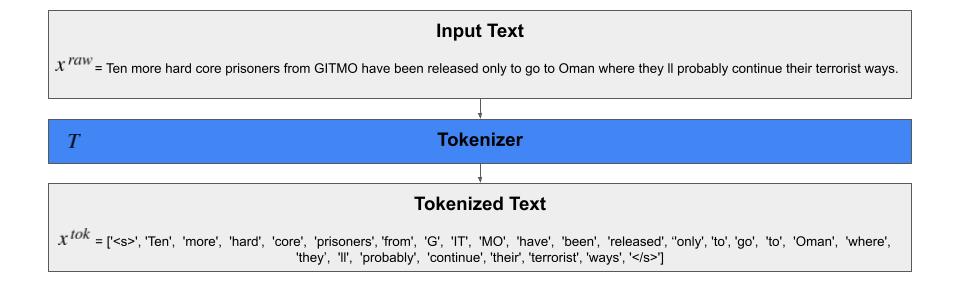
\includegraphics[scale=0.5]{InputTokenizationPipeline.png}
    \caption[The tokenization pipeline for a textual input.]{The tokenization pipeline for a textual input.}
    \label{fig:InputTokenizationPipeline}
\end{figure}
In order to feed the input to the model, we need numeric representation which can be obtained by various techniques. One widely used approach is the BoW representation which produces features based on the number of occurrences of a word or token. An alternative BoW representation uses the presence or absence of words in the vocabulary instead of frequencies. A more sophisticated approach is \emph{Word2Vec}, which encodes words into numeric values by learning word associations. From the perspective of the representation of a word, \emph{Word2Vec} can capture different degrees of similarity between words allowing for the preservation of semantic and syntactic relationships~\parencite{Word2Vec_Mikolov}. It is clear that the transformation of words into numeric vectors is a very crucial stage for FND since we need to maintain as much contextual information as possible. Nevertheless, the SOTA is an even more sophisticated approach called \emph{Transformer}, which is the building block of many powerful language models such as BERT.\\
We denote the space of raw label $Y^{raw} = \{"fake", "real"\}$, with $y^{raw} \in Y^{raw}$. We employ a label mapping function $\psi: Y^{raw} \mapsto Y$ that maps raw labels to classes, where $Y \in \mathbb{R}^2$ with,
\begin{center}
    \[\psi(y^{raw}) = y =
        \begin{cases}
            0, & if \;\; y^{raw} = "fake" \\
            1, & otherwise                \\
        \end{cases}
    \]
\end{center}
\begin{definition}[\emph{Classifier}]
    A classifier $f:X \mapsto Y$ is a function that outputs predicted scores $f(x)_y$ for each class $y$ for a given input $x$.
\end{definition}
Our classifier is a language model that was trained on a large corpus and a news dataset that contain fake and real news. It will predict whether a news piece is real or fake by assigning each label a probability.
\begin{definition}[\emph{Prediction}]
    A prediction $\hat{y}$ is the maximum of predicted scores $f(x)_y$ of a classifier.
    \begin{center}
        $\hat{y} = argmax_{y \in Y} f(x)_y$
    \end{center}
\end{definition}
We use a neural network classifier that consists of several layers and a complex architecture. Our model is able to work with large vocabularies and can classify news pieces based on various features.
\begin{definition}[\emph{Neural Network Classifier}]
    A neural network classifier is a \emph{classifier} $f$ that consists of layers $l$ with $1 \leq l \leq L$, where $L$ denotes the number of layers. Each layer has a set of units $a_i^{(l)}$, with $i$ denoting the position of the unit in layer $l$. We say that between two units, $a_i^{(l)}$ belonging to layer $l$ and $a_j^{(l+1)}$ belonging to layer
    $l+1$ have a weight value $w_{ij}^{(l)}$ that connects them. Along with a non-linear activation function $\sigma$, we
    can define the value of the $j$-th unit $a_j^{(l+1)}$ in terms of weights and unit values from the previous layer for an FCN, with $N$ as the number of units in layer $l$.
    \begin{center}
        $a_j^{(l+1)} = \sigma(\sum\limits_{i=1}^{N} a_i^{(l)} w_{ij}^{(l)})$
    \end{center}
\end{definition}
Neural networks are very powerful models. They can train millions of parameters using matrix multiplications, gradient-based optimization methods, and a fruitful set of other techniques, some of which will be discussed later. Neural networks iteratively optimize the weights between layers so that the produced output is as close to the desired output. This is achieved by using optimization methods, such as \emph{Gradient Descent} (GD)~\parencite{GD_Cauchy}, \emph{Stochastic Gradient Descent} (SGD)~\parencite{SGD_Robbins}, \emph{Adaptive Moment Estimation} (Adam)~\parencite{Adam_Kingma} that minimize the loss function defined for the problem. While many optimization methods are available for neural networks, we do not examine any of them.\\
\begin{figure}
    \centering
    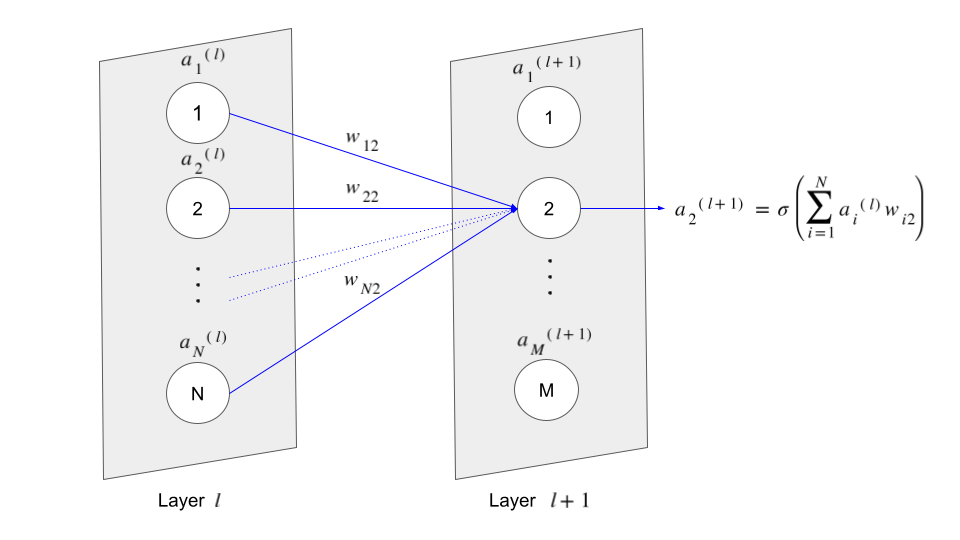
\includegraphics[scale=0.43]{NN_LayerRepresentation}
    \caption[Units and layers of an FCN.]{Units and layers of an FCN. For brevity, arrows and weights are only drawn for $a_2^{(l+1)}$.}
    \label{fig:NN_LayerRepresentation}
\end{figure}
For classification problems, we adopt a layer called \emph{Softmax}~\parencite{Softmax_Bridle} that outputs the predicted scores $f(x)_y$ for each class $y$ by normalizing outputs $Z_y(x)$ from the previous layer.\\
\begin{center}
    $f(x)_y = \dfrac{exp(Z_y(x))}{\sum\limits_{{y'} \in Y} exp(Z_{y'}(x))}$
\end{center}
The FCNs are the plainest architectures for neural networks. In an FCN, all units are connected. This means that there is a weight between each unit of the FCN and each unit of its previous layer. They are very straightforward to construct. Nevertheless, the usage of these architectures for modeling sequences is not preferred due to the exponential number of trained parameters. Instead, when modeling sequences like sentences and documents, a common approach is to adopt RNNs. RNNs allow previous outputs to be used while having hidden states. This permits information to pass through the sequence. However, vanilla RNNs are not powerful enough to represent long-term dependencies~\parencite{LearningLongTermDependenciesHard_Bengio} and suffer from vanishing/exploding gradients~\parencite{OnTheDifficultyOfTrainingRNNs_Pascanu}. \emph{Long Short-Term Memory} (LSTM)~\parencite{LSTM_Hochreiter} addresses the shortcomings of RNNs. The idea is to keep a cell state updated with the previous cell's state. This cell state is passed to the consequent cells to form a chain representing the document. More precisely, each cell corresponds to a token whose information will be shared with subsequent tokens by the propagation of cell states. This approach is indeed very useful for long documents since news articles tend to be long and their sentences contextually relevant. LSTM is usually used in different variations based on the same idea. For instance, a consequent study by~\citeauthor{LSTMPeephole_Gers} (\citeyear{LSTMPeephole_Gers}) has extended LSTMs with \emph{peephole connections}. LSTMs have been proven to deliver a good performance in NLP tasks such as \emph{speech recognition}~\parencite{AchievingHumanParityinConvSR_Wayne}. LSTMs perform well; however, they are being replaced with attention-based models due to long training times and large memory requirements during training.\\
One last thing to discuss is how the models are trained in terms of supervision. \emph{Supervised} models are trained with label data. \emph{Unsupervised} models work with unlabeled data and aim to find patterns in the data. An exciting setting is \emph{semi-supervised} models. These models are often provided with small amounts of labeled data and large amounts of unlabeled data for training. There are two settings for semi-supervised learning. \emph{Transductive} learning aims to predict unlabeled data, whereas \emph{inductive} learning samples unlabeled data from the same distribution to
infer the label~\parencite{LearningByTransduction_Gammerman}.\\
To summarize, we first outlined the process of a text becoming a numeric vector for a model. Then we discussed the classification steps and recapped the formation of neural networks. Finally, we argued about more capable model architectures employed in language models. Next, we will introduce the attention mechanism and Transformer models.

\subsection{Transformer Architecture}
\label{subsec:newsContentModels_TransformerArch}
Transductive learning has been successfully utilized along with the encoder-decoder structure in many language
tasks~\parencite{S2SLearningWithNNs_Sutskever, LearningPhraseRepresentations_Cho, AttentionIsAllYouNeed_Vaswani}. Transduction is first proposed by~\citeauthor{LearningByTransduction_Gammerman} (\citeyear{LearningByTransduction_Gammerman}) to counteract the unlabeled data problem. In contrast to supervised learning, transductive learning does not require all data to be labeled. Instead, it utilizes the clustered behavior of data. Transductive learning assigns labels to unlabeled data using the gaps between different clusters and a small set of labeled data. Transduction in sequence prediction is defined as a task where input sequences are transformed into output sequences~\parencite{SequenceTransdutionWithRNNs_Graves}. Transformer models are encoder-decoder structured language models that are designed for sequence transduction.\\
~\citeauthor{LearningPhraseRepresentations_Cho} (\citeyear{LearningPhraseRepresentations_Cho}) proposed an encoder-decoder structure that takes into account the order of words. This encoder-decoder structure consists of one RNN as the encoder and one RNN as the decoder. The encoder maps an input sequence to a fixed-length vector, and the decoder maps this fixed-length vector to a target sequence. Transformer architecture adopts a similar approach that employs feed-forward and Multi-Head Attention layers in both encoder and decoder, which is illustrated in Fig.~\ref{fig:transformerArchitecture} with N=6 stacks of encoders and decoders.\\
In order to reduce sequential computation, CNNs have been adopted as building blocks that parallelly compute hidden representations for all input and output positions~\parencite{AttentionIsAllYouNeed_Vaswani}. Although aimed to reduce computation, the number of operations to convey information from one random input or output to  the other increases linearly in ByteNet~\parencite{ByteNet_Kalchbrenner} and logarithmically in ConvS2S~\parencite{ConvS2S_Gehring}.\\
Contrary to CNNs, Transformers fix the number of operations by averaging attention-weighed positions, which decreases the effective resolution. However, this decrease in resolution is alleviated by using multi-head attention~\parencite{AttentionIsAllYouNeed_Vaswani}.
\begin{figure}
    \centering
    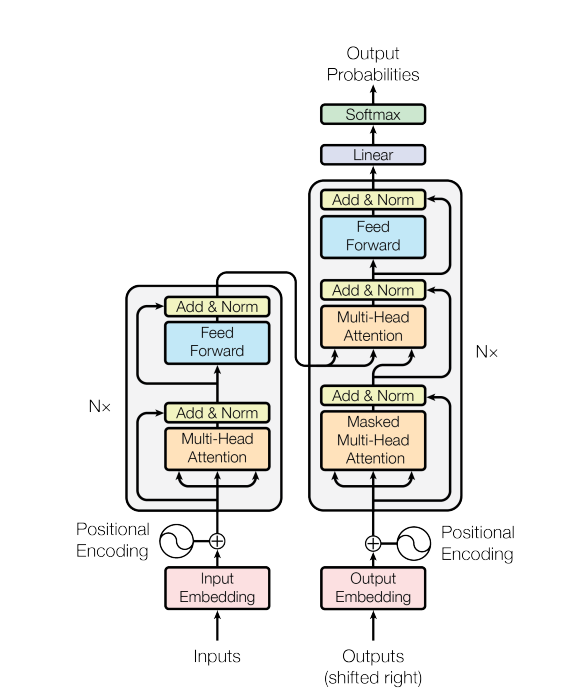
\includegraphics{TransformerArchitecture.png}
    \caption[The Transformer model architecture.]{The Transformer model architecture (N=6). Figure obtained from~\parencite{AttentionIsAllYouNeed_Vaswani}.}
    \label{fig:transformerArchitecture}
\end{figure}
Initially suggested in the decoder of the model proposed by~\citeauthor{NeuralMachineTranslationByJointlyLearning_Bahdanau} (\citeyear{NeuralMachineTranslationByJointlyLearning_Bahdanau}), an attention mechanism works similarly to human attention; it learns to put more importance on some words that convey the relevant information about the sentence. The attention mechanism that ~\citeauthor{NeuralMachineTranslationByJointlyLearning_Bahdanau} (\citeyear{NeuralMachineTranslationByJointlyLearning_Bahdanau}) use is called \emph{additive attention}. Inspired by additive attention,~\citeauthor{EffectiveApproachesToAttentionBased_Luong} (\citeyear{EffectiveApproachesToAttentionBased_Luong}) proposed a different approach called \emph{dot-product attention}, a form  that is also used in Transformer architecture.\\
% It does so by means of a context vector that depends on a sequence of \emph{annotations}. An annotation $h_i$ for a word (or token) $x_i$ contains information about the complete input sentence but with a focus on the words that are closer to the word $x_i$. The context vector $c_i$ for word $x_i$ is obtained as a weighted sum of all these annotations $h_i$~\parencite{NeuralMachineTranslationByJointlyLearning_Bahdanau}:
% \begin{center}
%     $c_i = \sum\limits_{j=1}^{|x|} \alpha_{ij} h_j$.
% \end{center}
% The weight $\alpha_{ij}$ is obtained by applying softmax to associated energy $e_{ij}$, which is an output of the alignment model $a$. The alignment model $a$ is a feed-forward neural network that jointly learns with the rest of the system. More precisely, we compute these values as follows~\parencite{NeuralMachineTranslationByJointlyLearning_Bahdanau}:
% \begin{center}
%     $\alpha_{ij} = \dfrac{e_{ij}}{\sum\limits_{k=1}^{|x|} exp(e_{ik})}$
% \end{center}
% where
% \begin{center}
%     $e_{ij} = a(s_{i-1}, h_j)$
% \end{center}
% with $s_i$ representing the current and $s_{i-1}$ the previous state of the
% model~\parencite{NeuralMachineTranslationByJointlyLearning_Bahdanau}. This is called \emph{additive attention}.\\
For Transformer models, the authors define the attention function as "\emph{mapping a query and a set of key-value pairs to an output, where the query, keys, values, and output are all vectors. The output is computed as a weighted sum of the values, where the weight assigned to each value is computed by a compatibility function of the query with the corresponding key.}"~\parencite{AttentionIsAllYouNeed_Vaswani}. The Transformer model employs two different attention mechanisms, namely, \emph{scaled dot-product attention} and \emph{multi-head attention}. Following~\parencite{AttentionIsAllYouNeed_Vaswani}, we denote that the input for the attention layers are matrices called queries $Q \in \mathbb{R}^{d_{model} \times d_k}$, keys $K \in \mathbb{R}^{d_{model} \times d_k}$, and values $V \in \mathbb{R}^{d_{model} \times d_v}$, with $d_k$ as the number of keys or values and $d_{model}$ being the model dimension. Scaled dot-product attention computes the dot product of all queries $q_i \in Q$ with all keys $K$ and scale the resulting weights with $\frac{1}{\sqrt{d_k}}$. After obtaining the softmax of the scaled weights, each weight is multiplied by the corresponding value to obtain attention values.
\begin{center}
    $Attention(Q, K, V) = softmax(\dfrac{QK^T}{\sqrt{d_k}})V$
\end{center}
The second attention mechanism, multi-head attention, uses multiple attentions, each of which uses a different learned linear projection of $Q$, $K$, $V$. Output of all of these attentions are then concatenated to obtain the final result. More precisely, it is computed as follows,
\begin{center}
    $MultiHead(Q, K, V) = Concat(head_1, head_2, \dots, head_h)W^{O}$
\end{center}
where each $head_i$ is calculated as,
\begin{center}
    $head_i = Attention(QW_i^Q, KW_i^K, VW_i^V)$
\end{center}
with projection for $Q$ as $W_i^Q \in \mathbb{R}^{d_{model} \times d_k}$, $K$ as $W_i^K \in \mathbb{R}^{d_{model} \times d_k}$, $Q$ as $W_i^V \in \mathbb{R}^{d_{model} \times d_v}$, and lastly, $W^{O} \in \mathbb{R}^{hd_v \times d_{model}}$~\parencite{AttentionIsAllYouNeed_Vaswani}.\\
We now outline each part of the Transformer model.\\
\begin{itemize}
    \item \emph{Encoder}: Consists of N=6 identical layers. Each of these layers has two sub-layers, the first of which uses multi-head attention and layer normalization~\parencite{LayerNorm_Ba} along with a residual connection~\parencite{ResidualConnection_He}. The second sub-layer consists of a feed-forward layer and layer normalization as well as a residual connection around the feed-forward layer~\parencite{AttentionIsAllYouNeed_Vaswani}
    \item \emph{Decoder}: Same as the encoder, this part is composed of N=6 layers. Additional to the previously discussed two sub-layers in the encoder, the decoder adopts a third sub-layer that computes the attention values over the output of the encoder. As it was done for the encoder, the decoder also utilizes layer normalization at the end of each sub-layer as well as the residual connection~\parencite{AttentionIsAllYouNeed_Vaswani}.
\end{itemize}
In the Transformer model, the embeddings are obtained through the embedding layer. All of the feed-forward networks in the sub-layers are position-wise, meaning that they are applied to each position separately and identically. These feed-forward networks use different parameters for each layer. Lastly, the positional encodings for input embeddings are calculated using sine and cosine functions of different frequencies~\parencite{AttentionIsAllYouNeed_Vaswani}. We will observe the effect of positional encodings when explaining the news content classifier.\\
In order to lay the foundations for the model we adopted, we have introduced its structure and mechanism. Next, we initially introduce details of BERT, then RoBERTa, and lastly DistilRoBERTa which is the base of our choice of news content classifier.

\subsection{Dataset and Model}
\label{subsec:newContentModel_DatasetAndModel}
We employ a fine-tuned version of the case-sensitive Transformer model DistilRoBERTa\footnote{\url{https://huggingface.co/GonzaloA/distilroberta-base-finetuned-fakeNews}} for our task of FND with news content. DistilRoBERTa is a distilled version of \emph{A Robustly Optimized BERT Pretraining Approach} (RoBERTa)~\parencite{RoBERTa_Liu}. It uses the same distillation procedure adopted to build  DistilBERT~\parencite{DistilBERT_Sanh} using \emph{Bidirectional Encoder Representations from Transformers} (BERT)~\parencite{BERT_Devlin}. This distillation procedure is referred to as \emph{knowledge distillation} and it compresses a model~\parencite{ModelCompression_Bucilua} - the teacher - by means of training a smaller model - the student - to reproduce the same behavior~\parencite{DistillingTheKnowledge_Hinton}. In our case, the teacher is  RoBERTa and the student is DistilRoBERTa. First, in order to examine the properties of RoBERTa, we discuss BERT in detail.\\
As the name suggests, the model architecture of BERT is a multi-layer bidirectional Transformer model. BERT uses BookCorpus~\parencite{BookCorpus_Yukun} and English Wikipedia as training datasets, with two training objectives, \emph{Masked Language Modeling} (MLM) and \emph{Next Sentence Prediction} (NSP).\\
NSP procedure is a binary classification loss that predicts whether two segments (sequences of tokens) are consecutive in
the original text. \emph{Positive} and \emph{negative} examples are sampled with equal probability in this process.
Positive examples are created by taking consecutive sentences from the text corpus, whereas negative examples
are generated by pairing segments from different documents~\parencite{BERT_Devlin,RoBERTa_Liu}.\\
MLM procedure applies the following for each sentence sampled from a document in the cumulative dataset.
\begin{itemize}
    \item Mask 15\% of the tokens.
    \item In 80\% of the cases, replace the masked tokens with [MASK].
    \item In 10\% of the cases, replace the masked tokens with a different random vocabulary token.
    \item In the remaining 10\% of the cases, the masked tokens are left unchanged.
\end{itemize}
RoBERTa is an optimized version of BERT. It was pretrained longer using longer sequences. RoBERTa uses MLM as the training objective but not NSP. Contrary to BERT, RoBERTa keeps a dynamic masking pattern that changes in training. It is
pretrained on the reunion of five datasets (three more datasets than BERT) that size up to 160 gigabytes (GB): BookCorpus~\parencite{BookCorpus_Yukun},
English Wikipedia~\parencite{EnglishWikipedia_Wiki},
CC-News~\parencite{CCNews_Nagel}, OpenWebText~\parencite{OpenWebText_Radford},
Stories~\parencite{ASimpleMethodForCommonsenseReasoning_Trinh}.\\
RoBERTa tokenizes texts using BPE with a vocabulary size of 50,000 and maximum sequence length (maximum number of tokens) as 512. The beginning and end of each document (news article) is marked with <s> and </s>, respectively. With MLM as the training objective and Adam~\parencite*{Adam_Kingma} as the optimizer, the model reaches better results than BERT. Additionally, it should be noted that these models are further trained for downstream tasks; thus, we refer to the training stage as pretraining to avoid any confusion.\\
DistilRoBERTa has the same general architecture as RoBERTa, but the number of layers is reduced by a factor of two, and the
\emph{token-type embeddings} and the pooler are removed. Then DistilRoBERTa is initialized with layers from the teacher.
The distillation is done with very large batches~\parencite{DistilBERT_Sanh}. Using RoBERTa as a teacher, the student DistilRoBERTa is pretrained on OpenWebTextCorpus~\parencite{OpenWebTextCorpus_Gokaslan}, a reproduction of OpenWebText~\parencite{OpenWebText_Radford}.\\
The model we employed from Huggingface used a dataset curated from different sources for training~\footnote{\url{https://huggingface.co/datasets/GonzaloA/fake_news}}. To clarify, this model was already trained, i.e., we did not train this model. Although there exist better datasets and news content classifiers, we opted for this particular model for two reasons. First, most SOTA news content classifiers do not provide their code and dataset to reproduce results. Second, since Transformers are SOTA and this particular trained model provides us with not only the dataset but also the train/test/validation splits, which allows us to analyze its explanation.\\
\textbf{Dataset.} The news content dataset comprises 40587 samples whose distribution of labels and train/validation/test splits are provided in Fig~\ref{fig:DatasetDistributionByLabelAndSplit}. The proportion of fake news is 46\%, which is a fair distribution between real and fake news instances. The train/validation/test split is the common practice 60\%/20\%/20\%.
\begin{figure}
    \centering
    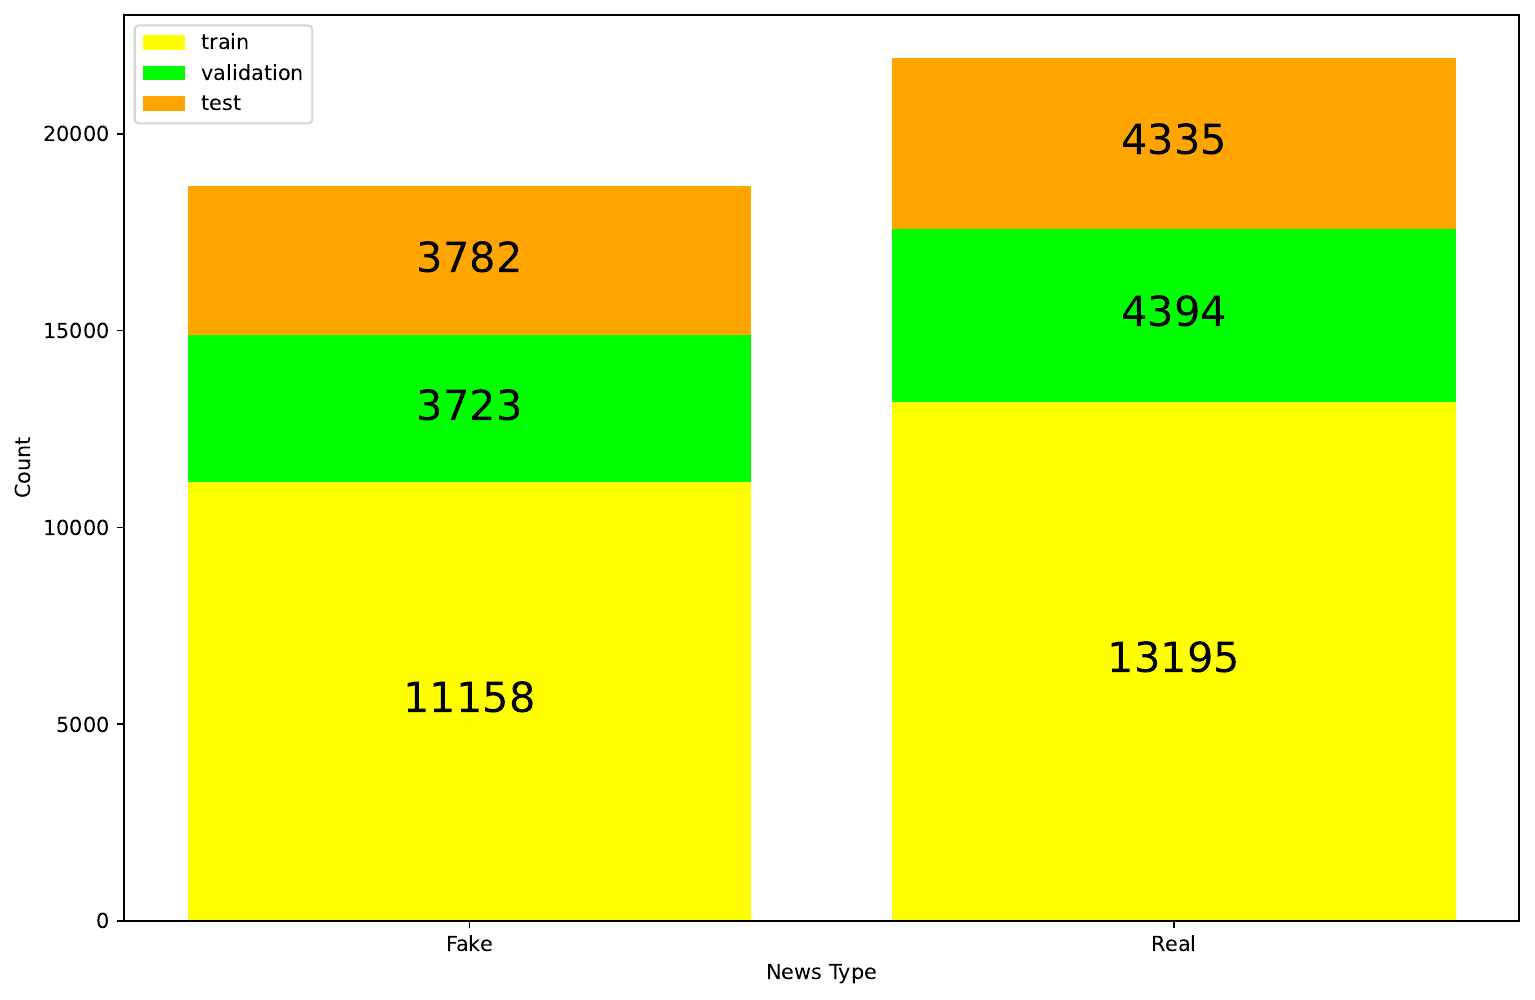
\includegraphics[scale=0.5]{DatasetDistrByLabelAndSplit.png}
    \caption[News content dataset distribution by label and train/validation/test split.]{News content dataset distribution by label and train/validation/test split.}
    \label{fig:DatasetDistributionByLabelAndSplit}
\end{figure}
We analyze the 500 most frequently occurring tokens in the dataset using a WordCloud~\parencite{WordCloud_Oesper} visualization for all samples of real and fake news separately in Fig~\ref{fig:WordCloudVisualizations}. From the visualization, we can observe that samples from both datasets contain the words "new", "state", "President", "Republican". In fact, the 500 most frequent tokens from fake news samples and real news samples share 63\% of tokens. Furthermore, we observe that one of the most frequent tokens is "Reuters" in real news instances. In fact, 95.93\% of real news samples contain the token coalition "(Reuters)". It is crucial to note that the idea of analyzing the frequency of keywords was initially formed once we started explaining the news content classifier. We will share how we draw this insight in the following section.\\
\begin{figure}
    \centering
    \subfloat[Fake news]{
\includegraphics[width=0.45\textwidth]{DatasetFakeFrequentTokensWordCloud.png}\label{subfig:WordCloud_DatasetFakeFrequentTokensWordCloud}}
    \hfill
    \subfloat[Real news]{
\includegraphics[width=0.45\textwidth]{DatasetRealFrequentTokensWordCloud.png}\label{subfig:WordCloud_DatasetRealFrequentTokensWordCloud}}
    \caption[WordCloud visualiations for most frequently occurring 500 tokens in both classes.]{WordCloud visualiations for most frequently occurring 500 tokens in samples of both classes.}
    \label{fig:WordCloudVisualizations}
\end{figure}\\
\textbf{Training.} Huggingface provides us with a \emph{TextClassificationPipeline} which allows feeding the dataset from Huggingface directly~\parencite{Transformers_Wolf}. This pipeline includes the tokenization process, DistilRoBERTa, and a classification layer. Our news content classifier has six layers, 12 attention heads, and a hidden size of 768 that totals up to 82M parameters (RoBERTa has 125M parameters). The vocabulary size is 50265, including special tokens. The model also uses a technique called \emph{dropout} which is a regularization technique that drops some connections between units of layers based on a probability value~\parencite{Dropout_Nitish}. All model hyperparameters are defined in~\ref{tab:newsContentModelHyperparameters}.\\
\begin{table}
    \centering
    \begin{tabular}{|l|l|}
        \hline
        Attention dropout probability           & 0.1                             \\
        \hline
        Batch size                              & 16                              \\
        \hline
        Epochs                                  & 3                               \\
        \hline
        Hidden layer activation function        & GELU~\parencite{GELU_Hendrycks} \\
        \hline
        Layer normalization factor ($\epsilon$) & 1e-05                           \\
        \hline
        Learning rate                           & 2e-05                           \\
        \hline
        Maximum position embeddings             & 514                             \\
        \hline
        Number of attention heads               & 12                              \\
        \hline
        Number of layers                        & 6                               \\
        \hline
        Vocabulary size                         & 50265                           \\
        \hline
        Weight Decay                            & 0.01                            \\
        \hline
    \end{tabular}
    \caption[Hyperparameters of the news content classifier.]{Hyperparameters of the news content classifier.}
    \label{tab:newsContentModelHyperparameters}
\end{table}
Note that the maximum position embeddings parameter also considers document start and end tokens when reporting its length. When feeding tokens $x^{tok}$ to the model, the start (<s>) and end (</s>) tokens are added by the model pipeline, so this leaves us with a maximum sequence length of 512, i.e., $|x|=512$. Note that in Figure~\ref{fig:InputTokenizationPipeline}, the length of $x$ is not 512 since the paddings are masked out in the attention mask before feeding the input $x$ to the model. We only illustrated values for tokens that exist, as pads will receive a value that has no effect on the calculation of the output, such as 0. \\
\textbf{Performance Evaluation.} The model is trained for three epochs with a batch size of 16, and Adam ($\beta_1=0.9$, $\beta_2=0.999$, $\epsilon=1e-08$) as the optimizer. The performance metrics for the model are provided in Table~\ref{tab:newsContentModelPerformanceMetrics}. To evaluate, the model performs very well on the dataset. Only 93 samples out of 8117 are classified incorrectly in the test split. Out of that 93 samples, 51 of them are fake news instances, and the rest are real news instances. However, good performance does not necessarily suggest that the model has learned its task. It might have found a simple pattern between fake and real news instances and based its prediction on this trivial feature. This is why explaining a model is crucial. We can inspect the news content classifier's behavior under different cases using explanation techniques.\\
\begin{table}
    \centering
    \begin{tabular}{c | c | c | c}
        \textbf{Accuracy} & \textbf{Precision} & \textbf{Recall} & \textbf{F1 score} \\
        \hline
        98.85\%           & 98.82\%            & 99.03\%         & 98.92\%           \\
    \end{tabular}
    \caption[The performance metrics for news content classifier.]{The performance metrics for news content classifier.}
    \label{tab:newsContentModelPerformanceMetrics}
\end{table}
We have laid out the foundations for the model we used to understand the news content model's learning mechanism. We reported the characteristics, training details, and performance of the news content classifier in this section. Our news content classifier seems to have learned its task very well. However, if this model was to be deployed for FND, then we need to see its performance in different settings, such as against adversarial approaches. We will explain the news content classifier by adopting methods from the coalitional game theory.

\section{Explaining News Content Models}
\label{sec:ExplainingNewsContentModels}
Although there exist models that can detect fake news with high accuracies, such as the news content classifier we adopted, the reasons behind this performance are seldom investigated. There could be a number of reasons, from dataset characteristics to wrong model architecture. Just by looking at a model's performance on a single dataset, one should not trust the model's spectacular performancee. Instead, look at the reasons to understand why this is happening. Is the model actually learning to distinguish between classes, or is it learning some other thing that we do not want? The explanation of this model can also tell the model's type in terms of style-based FND approaches. Does the news content classifier capture features based on objectivity or deception? In order to answer questions like these and more,~\citeauthor{AUnifiedApproach_Lundberg} (\citeyear{AUnifiedApproach_Lundberg}) propose a unified framework in which any model (except GNNs) can be explained.\\
We start this section by describing how the Shapley Additive exPlanation (SHAP) framework helps explain a model. After examining the SHAP framework, we utilize it for the news content classifier and examine the reasons behind its performance by conducting several experiments.\\
\subsection{The SHAP Framework}
\label{subsec:ExplainingNewsContentModels_SHAPFramework}
The SHAP framework aims to explain a prediction of a single input instance $x$ by computing Shapley values from coalitional game theory. These values correspond to the contribution of each input feature to the prediction made for $x$~\parencite{InterpretableMachineLearning_Molnar}. Specifically, we are interested in SHAP's ability to capture local explanations
for our news content classifier. Fortunately, SHAP provides explanation frameworks for a variety of models, including DNNs. In order to handle DNNs, SHAP improves methods from DeepLIFT to produce DeepSHAP. However, DeepSHAP is not compatible with Transformer models. Thus, we use a model-agnostic explanation model provided in the SHAP framework, namely the partition explainer. We begin with introducing Shapley values which are then converted to Owen values via feature coalitions. We will examine how Owen values and Shapley values are connected.\\
As before, let us denote our news content classifier to be explained as $f$ and its input as $x$. We focus on local explanations built for a single prediction $\hat{y} = f(x)$ based on one input $x$. An explanation model $g$ employs a simplified input $x'$, which is the output of a mapping function $h_x(x') = x$ that maps $x$ to $x'$. Each $h_x(x')$ is defined individually for each $x$. If two simplified inputs are similar $x' \sim z'$ then local methods aim to guarantee the approximation $g(z') \approx f(h_x(z'))$~\parencite{AUnifiedApproach_Lundberg}.\\
The general framework is built upon \emph{additive feature attribution methods}. These methods \emph{have an explanation model that is linear of binary variables}~\parencite{AUnifiedApproach_Lundberg}.\\
\begin{center}
    $g(z') = \phi_0 + \sum\limits_{i=1}^M \phi_i z_i'$
\end{center}
where $z' \in \{0, 1\}^M$, $M$ denotes the number of simplified input features, and $\phi_i \in \mathbb{R}$ feature relevance score of feature $i$~\parencite{AUnifiedApproach_Lundberg}. Note that $\phi_0$ corresponds to the base value, and can be used as an indicator to detect the bias in a model. Additive feature attribution methods have three desired properties. The first, local accuracy, states that \emph{the explanation model} $g(x')$ \emph{matches the original model} $f(x)$ \emph{when} $x = h_x(x')$~\parencite{AUnifiedApproach_Lundberg}. The second property is missingness, and it states that the features not included in the input should have no impact~\parencite{AUnifiedApproach_Lundberg}. The last property, consistency describes that if a simplified feature $x_i' \in x'$ have a greater impact in model $f'$ than the model $f$, then the feature $x_i$ should be assigned at least the same or a higher value for its contribution~\parencite{AUnifiedApproach_Lundberg}. \\
The computation of each $\phi_i$ involves a similar process to the calculation of classic Shapley regression values~\parencite{AnalysisOfRegressionInGameTheory_Lipovetsky}:
\begin{center}
    $\phi_i(f, x ) = \sum\limits_{z' \subseteq x'} \dfrac{|z'|! (M - |z'| - 1)!}{M!} [f_x(z') - f_x(z' \setminus i)]$
\end{center}
where $z' \setminus i$ implies $z_i' = 0$, $|z'|$ is the number of non-zero elements in $z'$, and $z' \subseteq x'$ denotes the set of vectors $z'$ whose non-zero elements are a subset of non-zero elements in $x'$~\parencite{AUnifiedApproach_Lundberg}.\\
% In the supplementary material of~\cite{AUnifiedApproach_Lundberg}, the authors define four axioms all of which Shapley values satisfy.
% \begin{enumerate}
%     \item \emph{Efficiency forces the model to correctly capture the original predicted value}~\parencite{AUnifiedApproach_Lundberg}
%     \item \emph{Symmetry states that if two features contribute equally to the model then their effects must be the same}~\parencite{AUnifiedApproach_Lundberg}.
%     \item \emph{Null effects} denotes that if a feature is missing in all subsets and this feature does not affect the outcome of the model, then this feature is ignored and its effect must be 0~\parencite{AUnifiedApproach_Lundberg}.
%     \item \emph{Linearity} states that if two models are written as a linear combination, then the sum of the effect of a feature in both models represent the effect of feature in the linear combination~\parencite{AUnifiedApproach_Lundberg}.
% \end{enumerate}
% Symmetry, null effects, and linearity are proven to be satisfied with the monotonocity axiom by~\citeauthor{MonotonicSolutionsOfCooperativeGames_Young} (\citeyear{MonotonicSolutionsOfCooperativeGames_Young}) and~\citeauthor{AUnifiedApproach_Lundberg} (\citeyear{AUnifiedApproach_Lundberg}). Therefore, we only need monotonocity and efficiency to be satisfied to constrain ourselves to using Shapley values. Owen values satisfy these constraints. 
Given a hierarchy of features that define feature coalitions, the partition explainer recursively computes Shapley values through them, and these Shapley values result in Owen values~\parencite{OwenValues_Owen}. Owen values are not the same as Shapley values, but if the coalition consists of the whole sentence or individual tokens, then Owen values and Shapley values become equal. A study~\parencite{TheOwenAndShapleyValue_Casajus} also shows that Shapley values are the expected Owen values for all symmetric distributions on all partitions. Owen values will help us detect token groups (if any exist) that play a significant role in the prediction of a model. Moreover, Owen values are computationally very cheap which, makes them more attractive.\\
We have summarized the foundations of the SHAP framework. As recommended in the source code documentation of SHAP\footnote{\url{https://github.com/slundberg/shap/}}, we use the partition explainer for our Transformer language model. Next, we will examine Owen values in action with our news content classifier.

\subsection{Explainability of the News Content Classifier}
\label{subsec:ExplainingNewsContentModels_ExplainingNewsContentClassifier}
Having introduced the required concepts, we now utilize them to explain the news content classifier using some real and fake news instances from the dataset. We adopt the partition explainer in order to understand how our Transformer model works. We specifically try to find its shortcomings so that we can decide whether it is a good idea to use this FND system in real cases.\\
\textbf{Initial Analysis.} We took a fake news example from the train split of the dataset and analyzed which tokens are deemed most important. The explanation provided by the partition explainer for our first fake news instance is illustrated in Fig.~\ref{fig:FakeNewsExample1_forceplot}. We can quickly observe that the base value is too high. In a normal setting, the base value should be around $0.5$ for a binary classifier. Apart from a high base value, the model is actually capturing sensible features. For example, it can detect a non-formal narrative using words like "ride", "hood", "The genius protestors".  Interestingly, punctuations such as ".", "," and ". "were given particularly high importance even though they should not contribute to the context of the news that much.\\
\begin{figure}
    \centering
    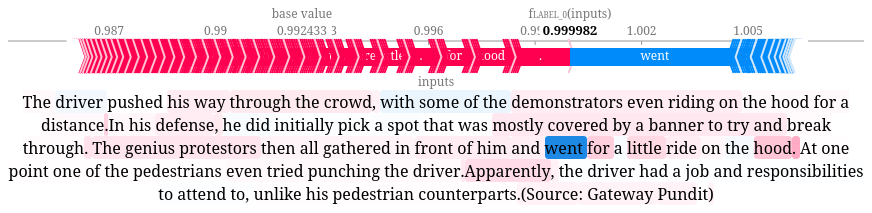
\includegraphics[scale=0.45]{FakeNewsExample1_forceplot.png}
    \caption[The explanation provided by SHAP partition explainer for our first fake news example.]{The explanation provided by SHAP partition explainer for our first fake news example. Example obtained by randomly selecting from our train split.}
    \label{fig:FakeNewsExample1_forceplot}
\end{figure}
% \begin{figure}
%     \centering
%     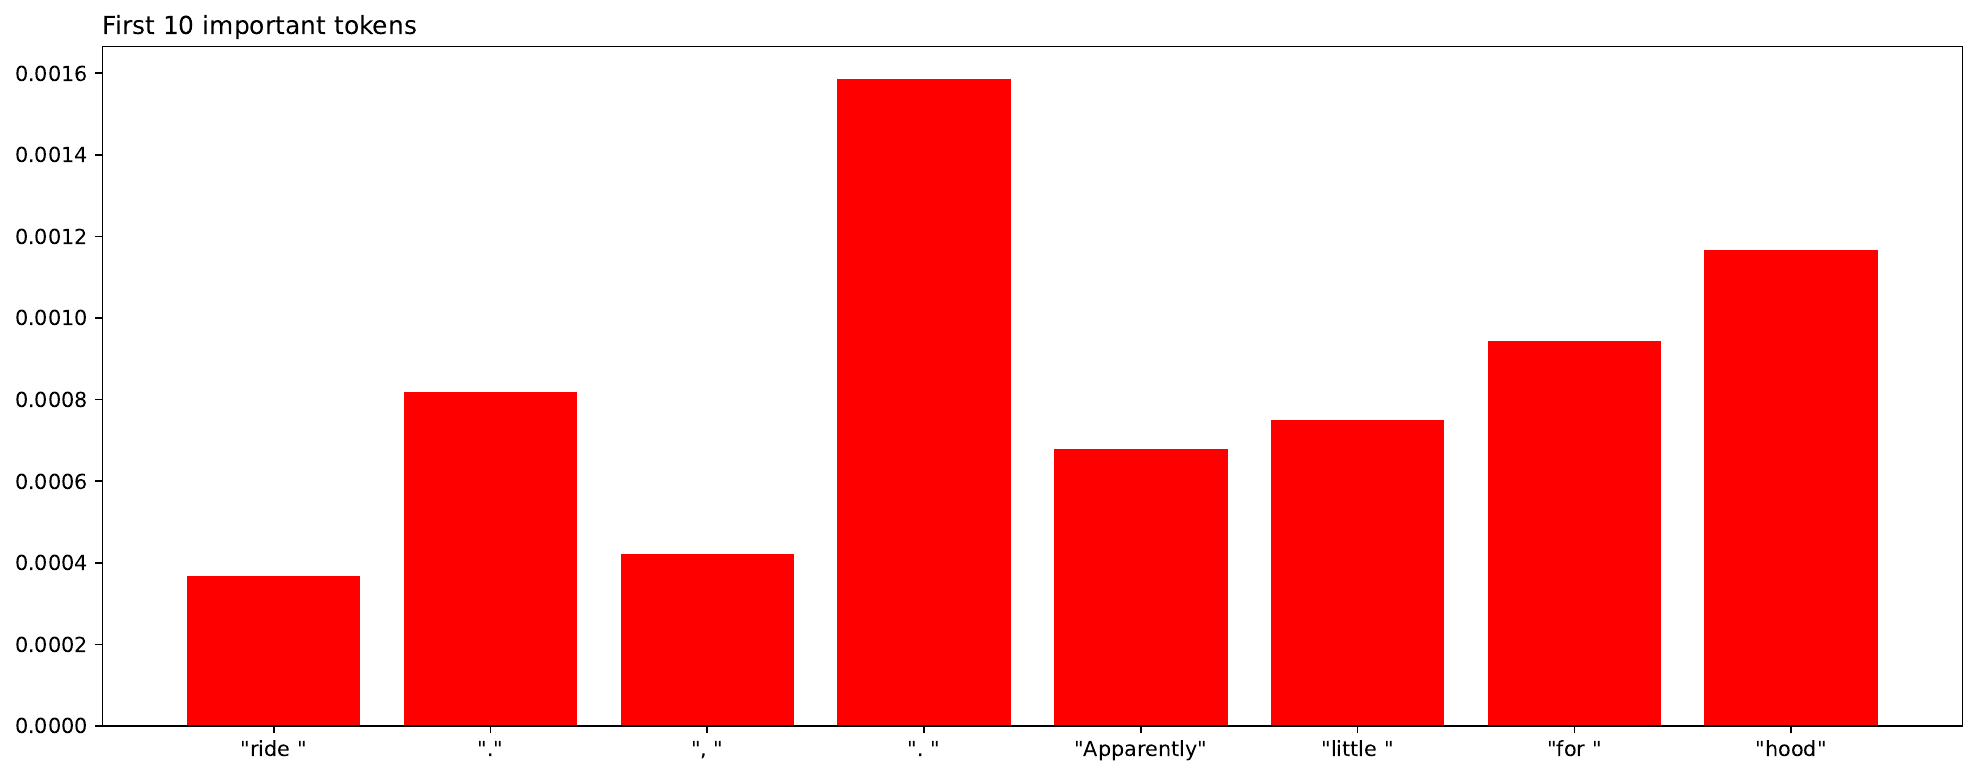
\includegraphics[scale=0.33]{FakeNewsExample1_barplot.png}
%     \caption[The barplot of the 10 highest Owen values and their tokens for the first fake news example.]{The barplot of the 10 highest Owen values and their tokens for the first fake news example. Since the news articles are long texts, we used a bar plot to visualize important tokens' Owen values.}
%     \label{fig:FakeNewsExample1_barplot}
% \end{figure}
We explain one more fake news instance from train split to see if the model behaves the same for that instance as well. The example is illustrated in Fig~\ref{fig:FakeNewsExample2_forceplot}. We can quickly observe that the model was able to capture non-formal speech again. We further examine how the tokens and coalitions are constructed. We see that "not a U." and "S. citizen." are separate coalitions. This implies that the tokenizer evaluated "U." and "S." as separate tokens. This issue might have occurred due to the punctuations between "U" and "S". Typically, one would expect "U.S." to be tokenized as one token, but the tokenizer failed to capture this. Following this issue, we realized that the tokenizer splits capitalized words into smaller units, which suggests the tokenizer is not capable of understanding most capitalized words. This might not be good for the news content classifier. In addition, the base value is again too high.\\
\begin{figure}
    \centering
    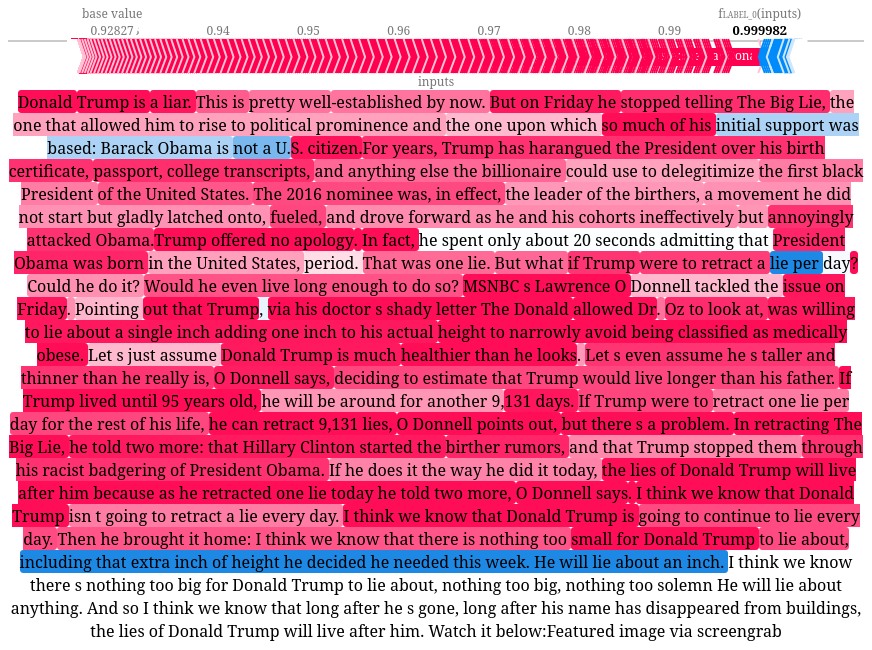
\includegraphics[scale=0.45]{FakeNewsExample2_forceplot.png}
    \caption[The explanation for the second fake news example.]{The explanation for the second fake news example. Observe that there are several coalitions between tokens such as "But on Friday he", "stopped telling The Big Lie" etc.}
    \label{fig:FakeNewsExample2_forceplot}
\end{figure}
\begin{figure}
    \centering
    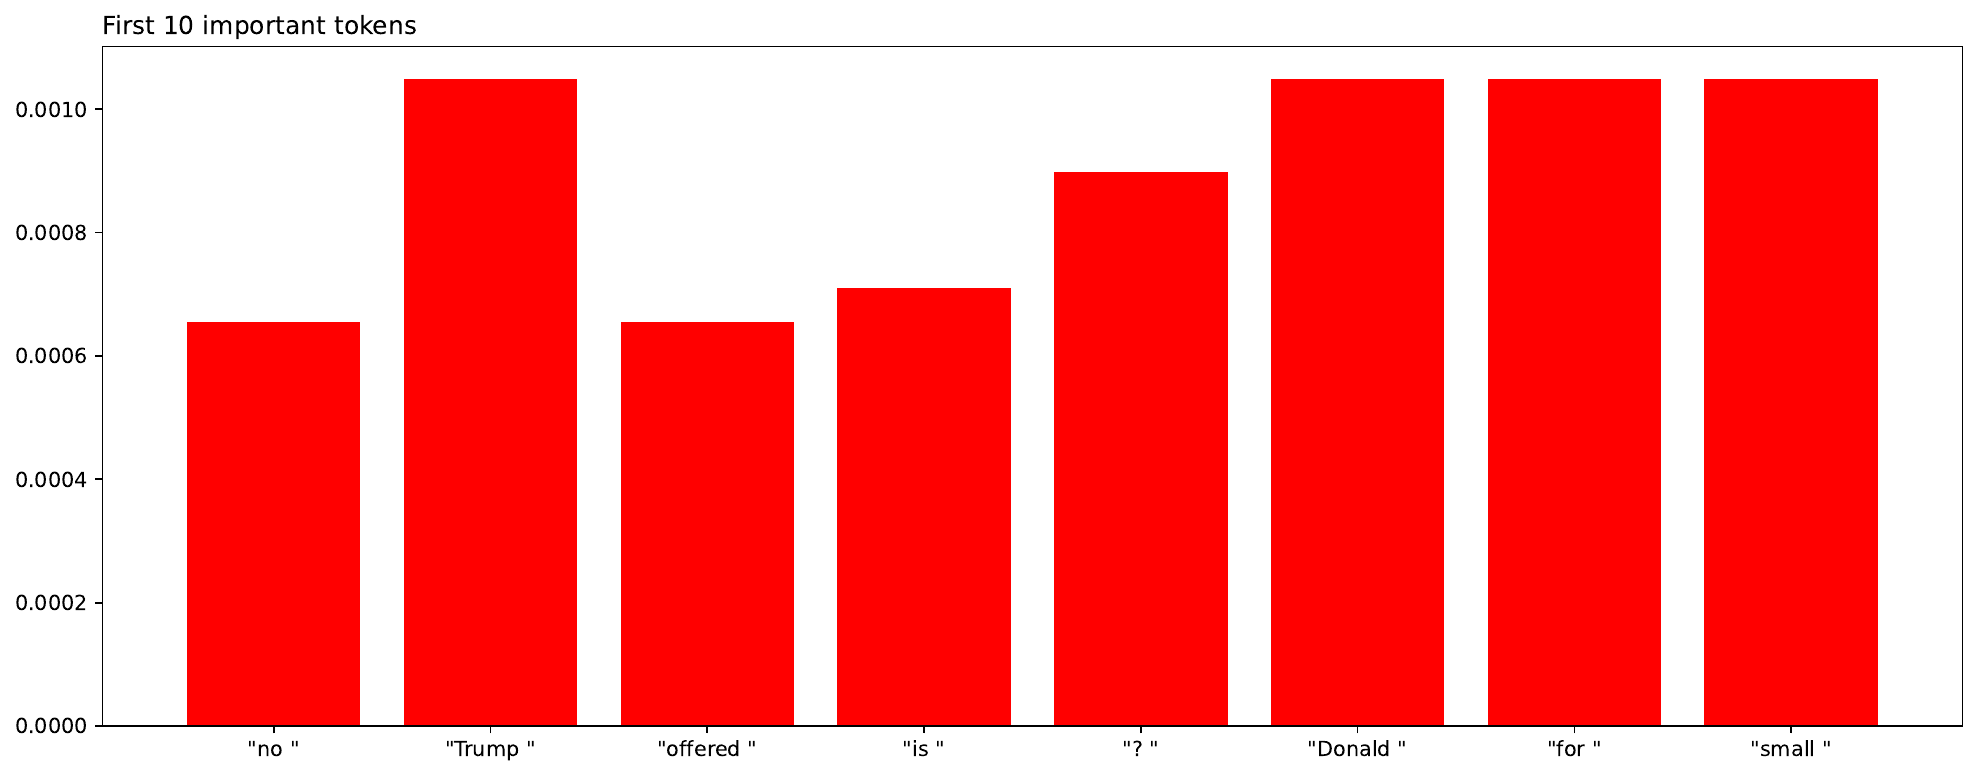
\includegraphics[scale=0.33]{FakeNewsExample2_barplot.png}
    \caption[The bar plot for the Owen values of the tokens in the second fake news example.]{The bar plot for the Owen values of the tokens in the second fake news example.  Since the news articles are long texts, we used a bar plot to visualize important tokens' Owen values.}
\end{figure}
We need to investigate why we obtain such high base values. Thus, to understand what the news content classifier thinks of the real news, we explain a real news instance from the train split. The example is shown in Fig.~\ref{fig:RealNewsExample1_forceplot}. We can easily see that the maximum share of Owen values go to three tokens: "(", "Reuters", ")". This suggests that the news content classifier has learned to distinguish news by source. In order to verify this intuition, we run one more real news example through the partition explainer. The explanation for the second example is illustrated in Fig.~\ref{fig:RealNewsExample2_forceplot}.\\
\begin{figure}
    \centering
    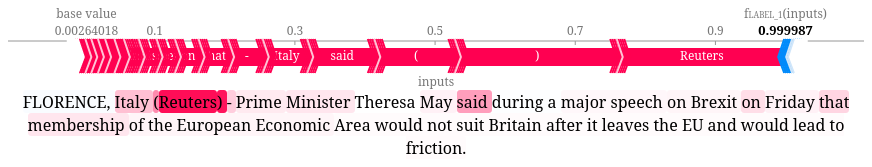
\includegraphics[scale=0.45]{RealNewsExample1_forceplot.png}
    \caption[The explanation for the first real news example.]{The explanation for the first real news example.}
    \label{fig:RealNewsExample1_forceplot}
\end{figure}
\begin{figure}
    \centering
    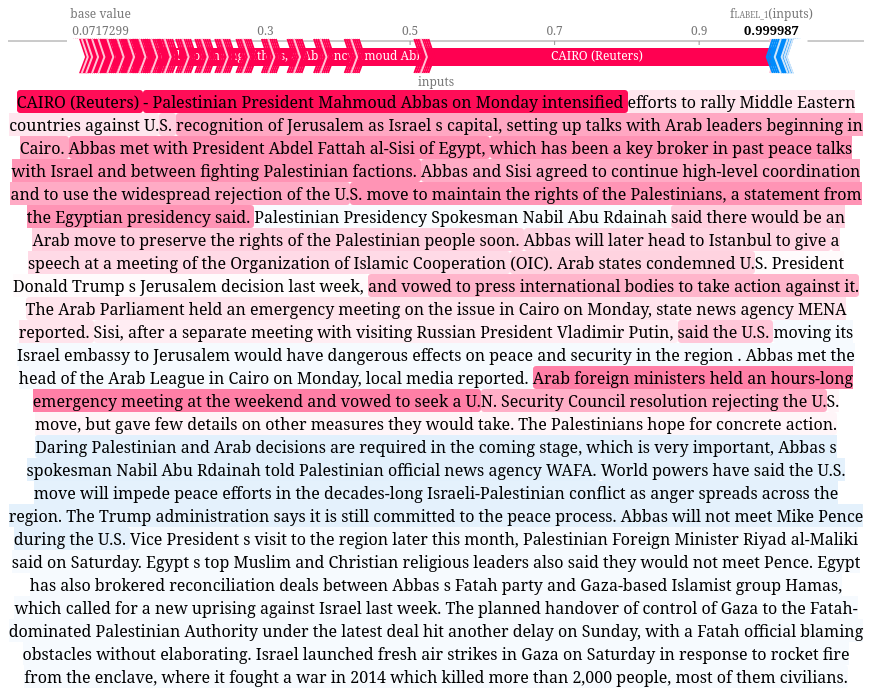
\includegraphics[scale=0.45]{RealNewsExample2_forceplot.png}
    \caption[The explanation for the second real news example.]{The explanation for the second real news example.}
    \label{fig:RealNewsExample2_forceplot}
\end{figure}
For the second example, we observe a coalition of tokens "CA", "IRO", " ", "(", "Reuters", ")". This coalition is given the highest Owen value of 0.48. The distribution of Owen values among tokens is illustrated in Fig.~\ref{fig:RealNewsExample2_barplot}. We can see that each token in the coalition was assigned almost equal Owen values. In two real news examples, the base value is really low. Again, one would expect around 0.5 for a binary classification setting.\\
\begin{figure}
    \centering
    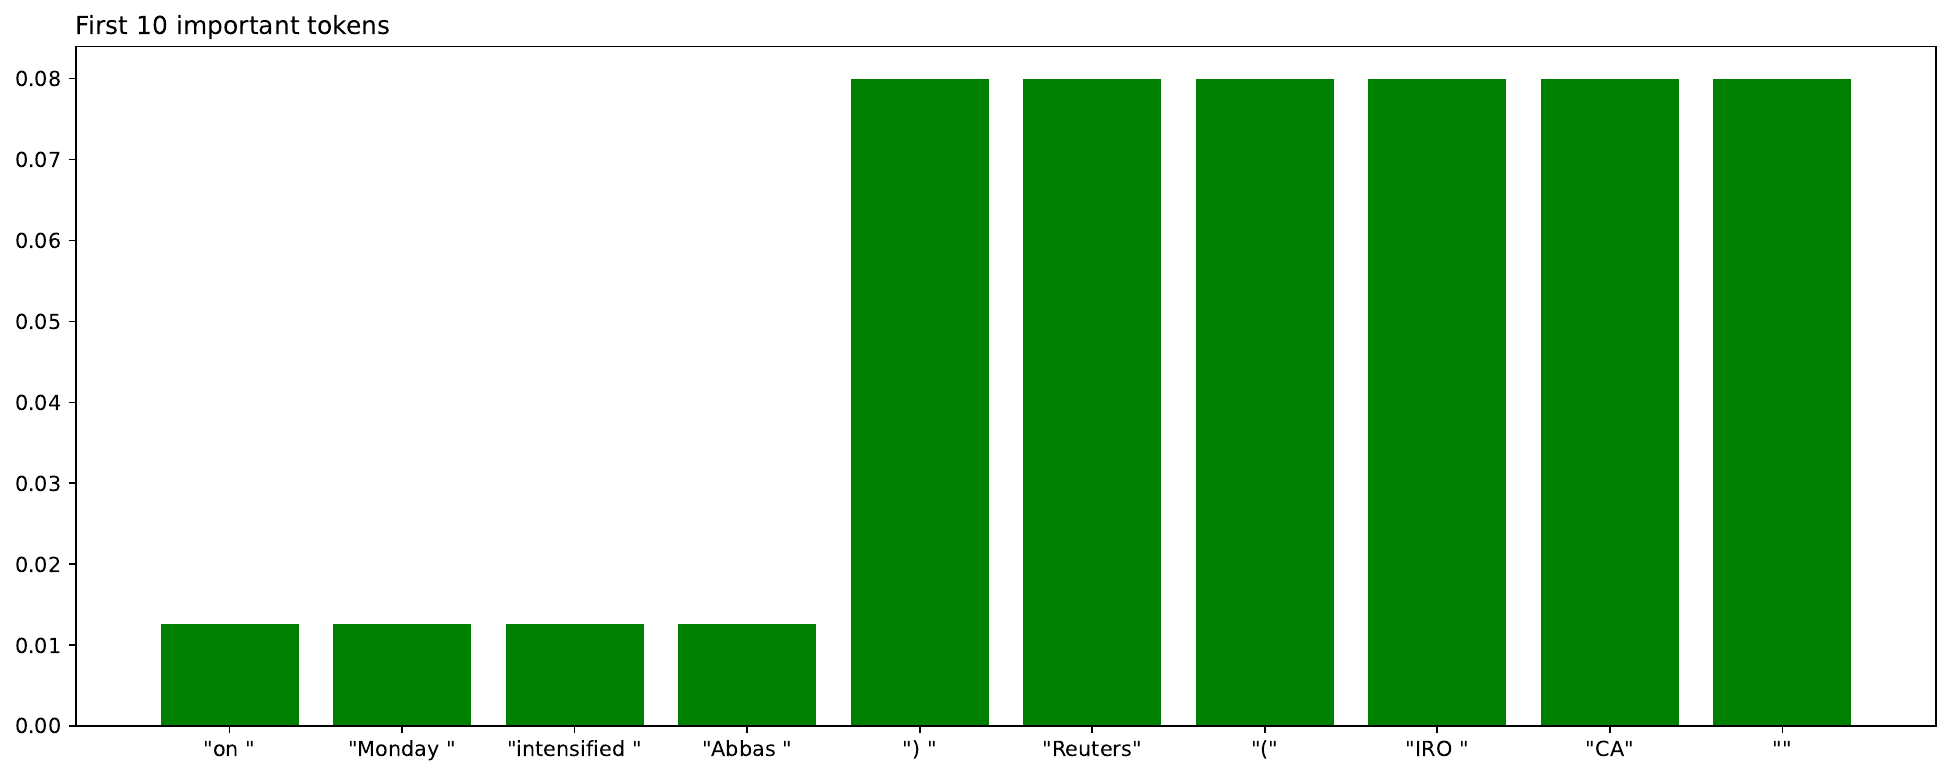
\includegraphics[scale=0.33]{RealNewsExample2_barplot.png}
    \caption[The bar plot of the 10 highest Owen values and their tokens for the second real news example.]{The bar plot of the 10 highest Owen values and their tokens for the second real news example.}
    \label{fig:RealNewsExample2_barplot}
\end{figure}
\textbf{Sensitivity Analysis.} Recall from~\ref{subsec:newContentModel_DatasetAndModel} that we reported that around 95\% of real news instances contained the text "(Reuters)". And also we expressed our concerns about the model basing most of its prediction on a couple of tokens. Now, let us consider that this model is deployed to detect fake news for a social platform. Once the adversaries realize this weakness of the model, then they could simply append "(Reuters)" to the beginning of their fake news and simply evade the detection. For a concrete example, see Fig.~\ref{fig:FakeNewsExample1Perturbed_forceplot}.\\
\begin{figure}
    \centering
    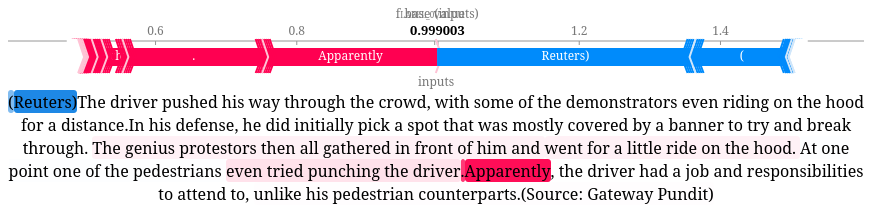
\includegraphics[scale=0.45]{FakeNewsExample1Perturbed_forceplot.png}
    \caption[The explanation for the perturbed first fake news instance.]{The explanation for the perturbed first fake news instance. This instance was predicted fake with more than 0.99 probability. We observe a very high base value as well. We see the negative effect of the token group "(Reuters)" on the force plot. Our intuition might be correct, however we might need a better alteration.}
    \label{fig:FakeNewsExample1Perturbed_forceplot}
\end{figure}
When we observe Fig.~\ref{fig:FakeNewsExample1Perturbed_forceplot}, we can easily see the adverse effect that the token "(" and the coalition "Reuters)" create is alleviated by assigning more Owen values to "Apparently" and ".". The model is still sure that this is a fake news instance. We might be required to adopt more complex adversarial approaches.\\
Knowing that the token group "(Reuters)" is never at the beginning of a real news article, we adopt more sophisticated changes in order to discover weaknesses of the model. We append a random string before "(Reuters)" and add the text " - " afterward, then append our fake news instance after this. This input sensitivity experiment shows that our intuition was correct for this instance. The explanation for this perturbation example is in Fig.~\ref{fig:FakeNewsExample1BetterPerturbed_forceplot}. We can observe that this fake news instance is now being predicted as real.\\
\begin{figure}
    \centering
    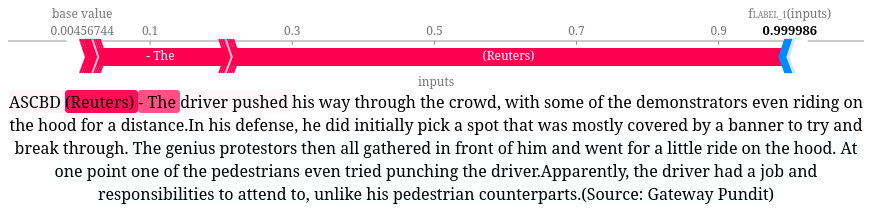
\includegraphics[scale=0.45]{FakeNewsExample1BetterPerturbed_forceplot.png}
    \caption[The explanation for the better perturbed first fake news instance.]{The explanation for the better perturbed first fake news instance. This instance was predicted real with over 0.99 probability. We can observe the dramatical probability change just by adding a couple words.}
    \label{fig:FakeNewsExample1BetterPerturbed_forceplot}
\end{figure}
\begin{figure}
    \centering
    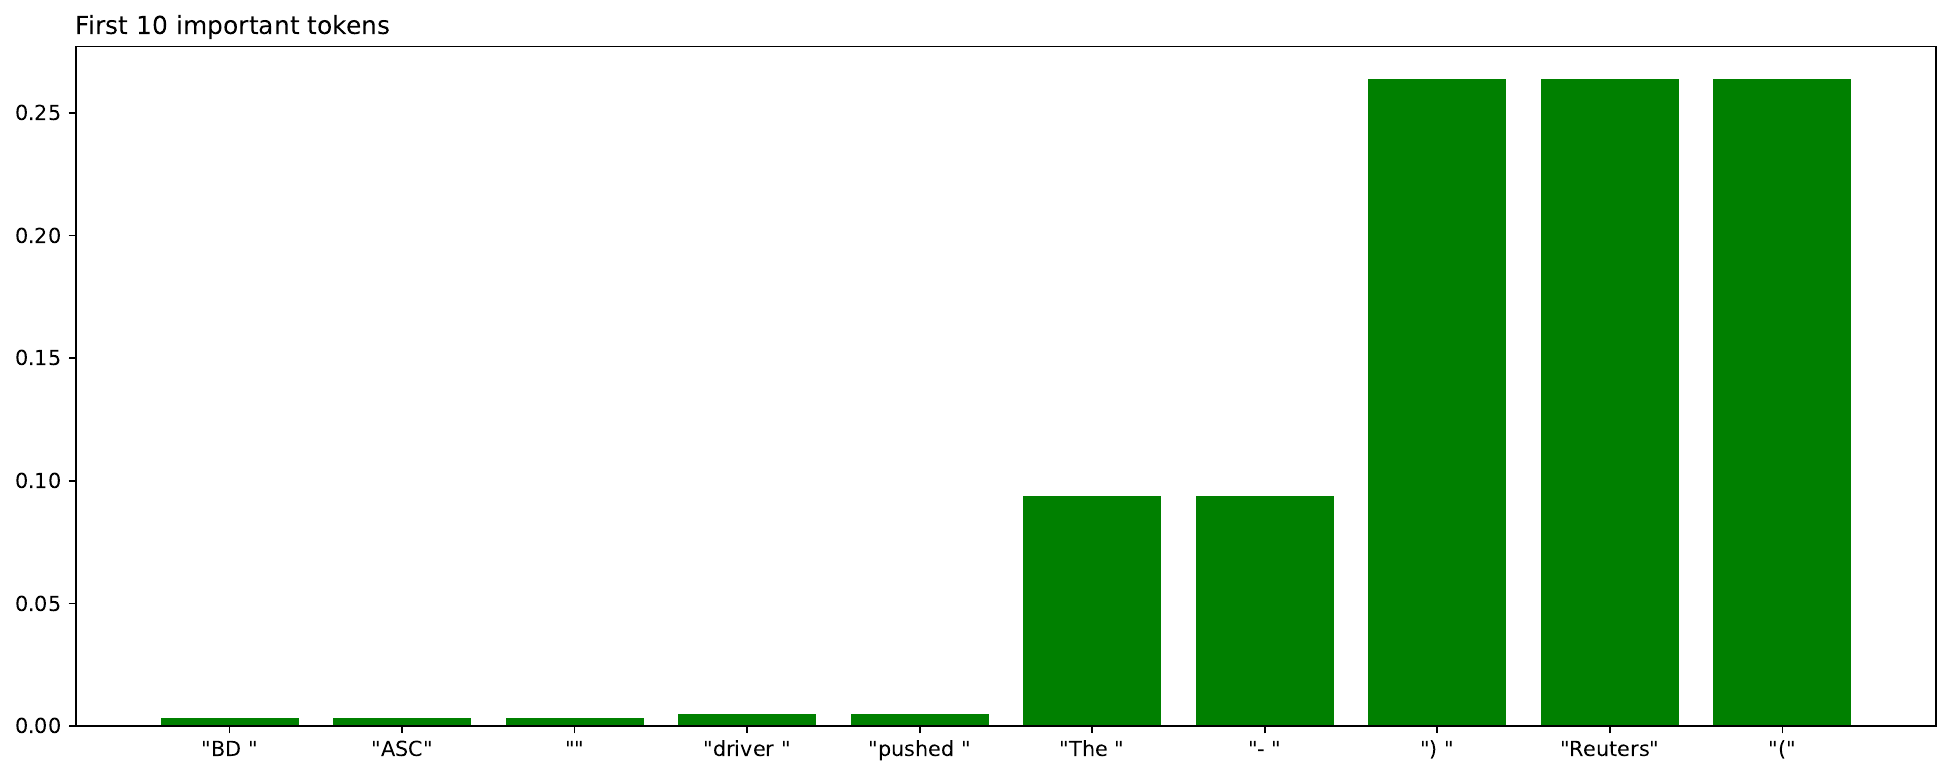
\includegraphics[scale=0.33]{FakeNewsExample1BetterPerturbed_barplot.png}
    \caption[The bar plot for the Owen values of better perturbed first fake news instance.]{The bar plot for the Owen values of better perturbed first fake news instance. Even a non-sense text like "ASCBD" is assigned one of the highest importance score.}
    \label{fig:FakeNewsExample1BetterPerturbed_barplot}
\end{figure}
\textbf{The Effect of The Model Architecture.} Now we can see the positional encodings' and attention mechanism's effect here. "ASCBD" is not a word, and it is tokenized as "ASC" and "BD" (can be seen in the x-axis of Fig.~\ref{fig:FakeNewsExample1BetterPerturbed_barplot}), with both tokens being assigned relatively large Owen values. Moreover, when the position of "(Reuters)" changes from the first to a later position, the model directly changes its mind. One more thing that comes to mind is the length of the text. Thus, we also applied the same technique to the second fake news example, whose feature relevance scores are better distributed. We got the same result for the second fake news example as well. We also observed similar behavior when explaining other training instances. We also tried using characters instead of character sequences and removing the space between "(Reuters)" and the initial character. The result was the same. This strongly suggests the model bases its predictions based on the existence and position of the token group "(Reuters)".\\
If we also consider the characteristics of DistilRoBERTa, we can see that the knowledge distillation process should be employed after the model is trained so that it can be deployed easily. Training a RoBERTa model with the cleaned dataset and then adopting the distillation process would be ideal. This way, more knowledge can be retained in the model.\\
We also conducted experiments with unseen data, but the results suggested the same outcome: clean the dataset and train again. Thus, we do not share the results from our unseen data experiment, as the results were parallel with the ones we have shared. In order to see the model's success without the existence of "(Reuters)" in real news, we need to train the news content classifier with the same hyperparameters in Table~\ref{tab:newsContentModelHyperparameters}, and the dataset should be changed such that the source part from the real news instances are removed, i.e., "$<location>$ (Reuters) -  $<newspiece>$" is changed to "$<newspiece>$" for real news.\\
We train the news content classifier by eliminating this issue from the dataset. We report the performance of the news content classifier in Table~\ref{tab:newsContentModelRetrainedPerformanceMetrics}.
\begin{table}
    \centering
    \begin{tabular}{c | c | c | c}
        \textbf{Accuracy} & \textbf{Precision} & \textbf{Recall} & \textbf{F1 score} \\
        \hline
        98.92\%           & 99.14\%            & 98.84\%         & 98.99\%           \\
    \end{tabular}
    \caption[The performance metrics for the retrained news content classifier.]{The performance metrics for the retrained news content classifier.}
    \label{tab:newsContentModelRetrainedPerformanceMetrics}
\end{table}
The performance stays the same, but let us inspect what the model has learned this time. To comparatively illustrate this, we ran the same examples we have introduced again and shared the force plot of the second fake news example in Fig.~\ref{fig:FakeNewsExample2_Retrained_forceplot}. Now that we have a lower base value for fake news, we can observe patterns caught by model in more depth. First, the high Owen values for the coalitions of contractions with the missing apostrophe, such as "MSNBC s", "doctor s", "Let s", "there s", "O Donnell" and "isn t" is the first pattern we observe in this instance. Second, full stops still get a relatively high Owen value. Moreover, even though the base value for fake news is decreased, it is still high.
\begin{figure}
    \centering
    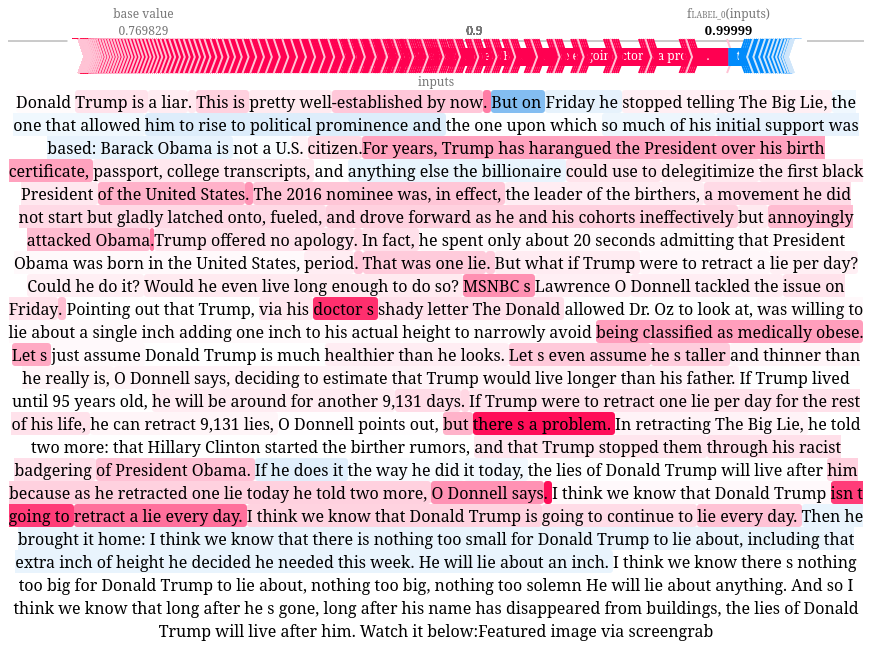
\includegraphics[scale=0.45]{FakeNewsExample2_Retrained_forceplot}
    \caption[The explanation of the second fake news instance for the retrained model.]{The explanation of the second fake news instance for the retrained model. Observe the lower base value and better distribution of Owen values.}
    \label{fig:FakeNewsExample2_Retrained_forceplot}
\end{figure}
To get a full understanding by comparing the explanation results, we also explain our second real news instance for our retrained model. The force plot of this explanation is shown in Fig.~\ref{fig:FakeNewsExample2_Retrained_forceplot}. We directly see the high base value, compared to Fig.~\ref{fig:RealNewsExample2_forceplot}, and also a better distribution of Owen values among the tokens and coalitions. The same detection for the lack of an apostrophe is also captured in this explanation. Coalitions like "Israel s", "Trump s", "Abbas s", "President s", and "Egypt s" have a large negative Owen value. This might suggest spelling mistakes such as leaving out the apostrophe are captured as informal by the news content classifier, even though these punctuations are removed in the tokenizer. There can be other reasons behind this behavior which can be uncovered by using explanation methods for other instances as well.
\begin{figure}
    \centering
    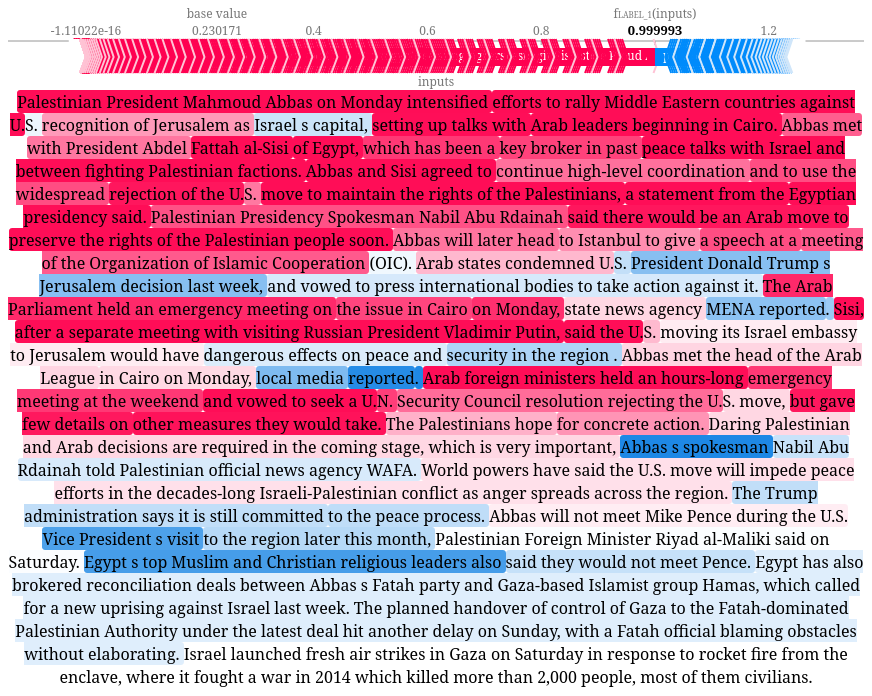
\includegraphics[scale=0.45]{RealNewsExample2_Retrained_forceplot}
    \caption[The explanation of the first fake news instance for the retrained model.]{The explanation of the first fake news instance for the retrained model. Observe the lower base value and better distribution of Owen values.}
    \label{fig:RealNewsExample2_Retrained_forceplot}
\end{figure}
We have seen that even though a model performs well, this doesn't mean that this model has learned the task. Since our news content classifier tries to distinguish between fake and real news using the patterns provided in the dataset, it is crucial to have a dataset that will not create the bias we observed. We used explanation techniques to uncover this issue with the news content classifier. We have seen the significance of adopting explanation methods to understand the behavior of the news content classifier. Thus, we have fulfilled \textbf{RO2} for news content classifiers.\\
Also, to fulfill \textbf{RO3} for this chapter, we report the understandability of the explanations provided by the partition explainer. Although we tried to explain long articles, the explanations were understandable, and the interactive behavior that allows viewing Owen values within coalitions helped us understand the impact of each token individually. With the help of bar plots, we were able to see the importance distribution between the first ten tokens. This allowed us to pinpoint the issue with the model even though it was performing very well. By utilizing simple visualization techniques, we were able to understand what the model had learned from the dataset. We used Python 3.7~\parencite{Python_Rossum}, PyTorch 1.11.0~\parencite{PyTorch_Paszke}, Transformers 4.19.2~\parencite{Transformers_Wolf}, SHAP 0.40.0~\parencite{AUnifiedApproach_Lundberg}, and Matplotlib 3.5.1~\parencite{Matplotlib_Hunter} for our implementations, visualizations, and experiments. The detailed usage of libraries, model explanation, and related work are provided in our GitHub repository\footnote{\url{https://github.com/sersery35/Explainability_of_FND_Models/tree/main/Huggingface}} \\
News content is highly related to the veracity of the news. Nonetheless, we might need more information to distinguish between fake and real news. In the next chapter, we introduce mixed approaches for FND in which we utilize news content data as well as social context data. Having this fusion of information proves to be very effective, as shown by~\citeauthor{UPFD_Dataset_Shu} (\citeyear{UPFD_Dataset_Shu}), models that use news content with social context are more successful than the models that utilize social context only.\\
% !TeX root = ../main.tex
% Add the above to each chapter to make compiling the PDF easier in some editors.

\chapter{Explainability of Mixed Approaches for Fake News Detection}\label{chapter:MixedApproachesForFND}

\section{Mixed Approaches}
\label{sec:mixedApproaches}
As discussed in Section~\ref{sec:fakeNewsDetection}, social media's interconnected nature leads to the fast dissemination of
fake news. When a news piece is shared, it propagates through social media by means of friendship networks. These networks
can be exploited to gather information about how fake news pieces spread. Moreover, users' historical information can prove effective when analyzing whether a news piece is real. This assumption stems from the psychological facts we discussed in Section~\ref{sec:fakeNewsDetection}. To recap, if a user is sharing fake news most of the time, then it is likely that the following news piece they will share will also be fake. Usually, fake news pieces are shared most within echo chambers, which gives rise to the quick spread of fake news.\\
There exist many different approaches to social context models. However, creating a dataset for social context models is a challenging task, as the amount of data to be collected can grow exponentially. Thus, we selected a dataset that provides us with social context information and news content. A graph dataset for our mixed approach model, \emph{User Preference-aware Fake Detection} (UPFD)~\parencite{UPFD_Dataset_Shu}, builds a propagation tree for each news using the users who retweeted the news. Nevertheless, in order to build a model that takes graphs as input, we can no longer rely on standard deep learning approaches because the graph data has a different structure. Thus, graph data is challenging to represent in the euclidean domain. Graphs hold node information as well as edge information between nodes, allowing to store rich relational data~\parencite{DeepLearningOnGraphs_Zhang}.\\
In this section, we lay out the foundations of graphs and GNNs. Then we investigate UPFD and report our findings. Lastly, we introduce our choice of mixed approach model and share its performance from our experiments.

\subsection{Overview of Graphs}
\label{subsec:mixedApproaches_OverviewOfGraphs}
In this section, we introduce definitions to cover graphs and different types of GNNs. However, we do not discuss each model type in detail due to GNNs' extensive background. Thus, we do not provide a notation for this section, but we give mathematical definitions when required.\\
Graphs are an example of \emph{non-euclidean} data, meaning that in contrast to \emph{euclidean} data, they can represent complex relations and entities more accurately than one or two-dimensional representations. Non-euclidean data used in GDL can be grouped into grids, graphs, groups, geodesics, and gauges, also called the 5G's of \emph{Geometric Deep Learning} (GDL)~\parencite{GeometricDeepLearning_Bronstein}. We are interested in only one G, graphs.
\begin{definition}[\emph{Geometric Deep Learning (GDL)}]
    A class of deep learning that aims to build models that can learn to predict on the non-euclidean domain.
\end{definition}
GDL is an extensive field covering various techniques that can be applied to the non-euclidean domain. Due to its complex nature, we do not provide a rigorous background on GDL. For a detailed background on GDL, we refer the reader to an extensive study on GDL~\parencite{GeometricDeepLearning_Bronstein}. We only discuss parts related to GNNs that we utilized. First, we define a graph.
\begin{definition}[\emph{Graph}]
    A graph is a non-euclidean type of data that represents the relations between entities.
\end{definition}
From the perspective of individual node connections, graphs can be categorized into two classes, \emph{directed} and \emph{undirected}. Directed graphs have direction information in their edges, i.e., the information flows strictly from one node to another. On the other hand, undirected graphs do not have this limitation. The information flow is bidirectional. Since we are only interested in undirected graphs like UPFD, we give preliminaries for an undirected graph.\\
Following standard notation on graphs, we define an undirected graph as $\mathcal{G} = (\mathcal{V}, \mathcal{E})$ with $\mathcal{V}$ as the set of nodes and $\mathcal{E}$ as the set of edges in a graph $\mathcal{G}$. We say that an edge $(v_i, v_j)$ exists between two nodes $v_i$ and $v_j$. Moreover, from the perspective of a graph's connectedness, two types of graphs exist: \emph{cyclic} or \emph{acyclic}. Simply put, cyclic graphs have cycles in them, i.e., they allow at least one node $v_i$ to have a series of different edges that creates a cycle back to node $v_i$. In contrast, acyclic graphs do not contain cycles. A concrete example of undirected acyclic graphs is trees, which strictly have one edge between two nodes.\\
When we look at graphs from node and edge type, we classify graphs as \emph{homogeneous} and \emph{heterogeneous} graphs. Homogeneous graphs have nodes and edges of the same type, whereas heterogeneous graphs have different types of nodes and edges. An example of a homogeneous graph is a social network in which the nodes are users, and the edges represent the friendship between two users. If we modify this social network into a more detailed version in which we choose to represent another relationship between users, such as colleagueship, then we would have a heterogeneous graph because there would be two types of edges in the graph.\\
Finally, if we consider graphs from a temporal aspect, we observe two kinds of graphs, \emph{static} and \emph{dynamic}. Static graphs stay the same over time. Their topology or features do not change. In contrast, dynamic graphs' features and topology vary  over time, thus making time an important factor when working with dynamic graphs.

\subsection{Graph Neural Networks}
\label{subsec:mixedApproaches_GraphNeuralNetworks}
GNNs are neural networks that can take graphs as input and produce predictions at three levels:
\emph{node-level}, \emph{edge-level}, and \emph{graph-level}. Node-level tasks include node classification, node
regression, and node clustering. Node classification aims to categorize nodes into classes. Node regression deals with
predicting continuous value for each node. Lastly, node clustering aims to group nodes into several clusters. Edge-level tasks consist of edge classification and link prediction. Edge classification tries to categorize an edge, and link prediction seeks to find whether there is an edge between two nodes. Graph-level predictions are graph classification, graph regression, and graph matching. In all these settings, the model needs to learn graph representations~\parencite{GNNsAReview_Zhou}.\\
In our experiments, we used a model that uses a convolutional layer called GraphSAGE~\parencite{GraphSAGE_Hamilton}. We also worked with a convolutional attention layer called \emph{Graph Attention} (GAT)~\parencite{GraphAttentionNetworks_Velickovic}. Nevertheless, due to the length of experiments and insight collection, we opted not to report our findings from our study with GAT. In order to cover the background of GNNs, we outline both, along with many others. We first examine the general framework.\\
\cite{GNNsAReview_Zhou} define three modules in a generic GNN model: the \emph{propagation module}, \emph{sampling module}, and \emph{pooling module}. The propagation module deals with information propagation between nodes so that the aggregated information can represent the features and topology of the graph. Propagation modules usually employ a \emph{convolution operator} or \emph{recurrent operator} to aggregate information from neighbors of nodes. These aggregated values are then used to update the representation of the nodes, edges, and graph. Additionally, these modules employ a skip connection that helps to alleviate the over-smoothing problem by collecting previous representations of nodes. A sampling module is used when the input graph is too large to handle propagation and before the propagation module. Lastly, pooling modules are employed when extracting information to represent high-level graphs.\\
We will primarily deal with the propagation module and the operations within. We do not discuss recurrent operations on graphs as their background is extensive and out of the scope of this thesis. We refer the reader to an extensive study by~\citeauthor{GNNsAReview_Zhou} (\citeyear{GNNsAReview_Zhou}) for a mathematical background on convolutions and other operations in the spectral domain. We will outline the behavior of convolutions on graphs in order to give sufficient knowledge for the models we used.\\
\textbf{Convolutions on graphs.} The idea of convolution operators is to generalize convolutions from another domain to the spectral domain. In general, there are two types of convolutional operations: \emph{spectral} and \emph{spatial}.\\
The first, spectral approaches, are based on graph signal processing and define their convolutional operators in the spectral domain~\parencite{TheEmergingFieldOfSignalProcessingOnGraphs_Shuman}. Spectral methods initially transform a graph signal $x$ to the spectral domain by the graph Fourier transform $\mathcal{F}$, then the convolution operation is applied. The output from convolution is transformed back with the inverse Fourier transform $\mathcal{F}^{-1}$. Now we summarize the mathematics behind this approach in order to convey the UPFD classifier's characteristics. Graph Fourier and inverse graph Fourier transform are defined as,
\begin{center}
    $\mathcal{F}(x) = U^T x$
\end{center}
\begin{center}
    $\mathcal{F}^{-1}(x) = Ux$
\end{center}
where $U$ is the eigenvalue matrix of normalized graph Laplacian $L = I_N - D^{\frac{-1}{2}} A D^{\frac{-1}{2}}$ with $I_N$ the identity matrix of dimension $N$, $D$ as the degree matrix, and $A$ as the adjacency matrix of the graph. $L$ is a real symmetric positive semi-definite matrix which helps us with factorization $L = U \Lambda U^T$ where $\Lambda$ denotes the diagonal eigenvalue matrix~\parencite{GNNsAReview_Zhou}. Now that we can convert our graph signal $x$ to the spectral domain and back, following~\citeauthor{AWaveletTourOfSignalProcessing_Mallat} (\citeyear{AWaveletTourOfSignalProcessing_Mallat}) and~\citeauthor{GNNsAReview_Zhou} (\citeyear{GNNsAReview_Zhou}), we can define the convolution operation $\star$ on $x$.
\begin{center}
    $g \star x = \mathcal{F}^{-1}(\mathcal{F}(g) \bigodot \mathcal{F}(x))$ \\ $= U(U^T g \bigodot U^T x)$
\end{center}
where $\bigodot$ stands for element-wise multiplication and $U^Tg$ is the convolution filter in the spectral domain. This can be further simplified into the basis function of spectral methods:
\begin{center}
    $g_w \star x = U g_w U^T x$
\end{center}
where $g_w$ is a diagonal learnable matrix. Essentially, all spectral methods use a convolutional filter $g_w$, but their choice of design creates a variety of approaches that are built upon each other. We only discuss the ones necessary for the UPFD classifier. The main idea of modern convolutional operators comes from approximating $g_w$ with $k$-th order Chebsyshev polynomials~\parencite{GNNsAReview_Zhou}. GCN adopts $k=1$ to avoid overfitting. Moreover, GCN introduces a renormalization trick to solve the exploding/vanishing gradient problem~\parencite{GCN_Kipf}. Further works like AGCN~\parencite{AGCN_Li} have employed a similar approach. Additionally, GCN is employed to an extent in spatial approaches~\parencite{GNNsAReview_Zhou}.\\
The second, spatial approaches, focus on the graph structure. They define convolutions directly on graph topology. Spatial approaches can be grouped into \emph{basic}, \emph{attention-based}, and \emph{framework}. Basic spatial approaches define convolution operations on the neighborhoods of different sizes. Neighborhoods are defined based on nodes as follows $\mathcal{N}_v$ for a node $v$. There exist several basic spatial approaches, such as the diffusion CNN (DCNN)~\parencite{DCNN_Atwood}, which describes the neighborhood for nodes using transition matrices and the learnable GCN (LGCN)~\parencite{LGCN_Gao}, which utilizes CNNs as aggregators by applying max pooling on neighborhood matrices.\\
Another example, GraphSAGE uses an inductive learning approach to sample and then aggregate features from a node's local neighborhood. GraphSAGE uniformly samples a fixed-size collection of neighbors then aggregates this collection to produce embeddings for the graph~\parencite{GraphSAGE_Hamilton}. More precisely, let us assume that we have learned the parameters of $K$ aggregator functions denoted as $\textsc{AGG}_k$, and a set of weight matrices $W^k$ where $\forall k \in \{1, \dots K\}$. $k$ can be referred to as layer or search depth. Then for each $k$ we go through all nodes $v \in \mathcal{V}$ and apply an aggregation and then an update. Concretely, at each $k$ and at each $v$, let $h_v^{k-1}$ denote the hidden state of a node $v$ at layer $k-1$. Following the same notation, we refer to the hidden state of a node's neighborhood $\mathcal{N}_v$ at layer $k$ as $h_{\mathcal{N}_v}^k$. GraphSAGE formalizes its aggregation and update operation at layer $k$ as:
\begin{center}
    $h_{\mathcal{N}_v}^{k} = \textsc{AGG}_{k}(\{h_u^{k-1}, \forall u \in \mathcal{N}_v\})$
\end{center}
\begin{center}
    $h_v^k = \sigma(W^k [h_v^{k-1} || h_{\mathcal{N}_v}^k])$
\end{center}
where $||$ denotes concatenation of two vectors, $[h_v^{k-1} || h_{\mathcal{N}_v}^k]$ concatenated vector and $\sigma$
a non-linear activation function. GraphSAGE employs three different aggregators: \emph{mean aggregator}, \emph{LSTM aggregator}, and \emph{pooling aggregator}. The mean aggregator collects sampled neighborhood information and takes the element-wise mean of the vector set $\{h_u^{k-1}, \forall u \in \mathcal{N}_v\}$. The inductive version also includes the previous layer representation of node $v$, $h_v^{k-1}$. LSTM aggregator uses an LSTM to collect neighborhood information. LSTMs are more expressive than mean aggregators. However, since LSTMs are not permutation invariant, i.e., they process
their inputs sequentially, they need a modification to work with unordered sets. Finally, the pooling aggregator first independently feeds each neighbor's vector to an FCN, then applies a pooling operation on the output.\\
The third, \emph{attention-based approaches}, utilize the same attention mechanism introduced in~\ref{subsec:newsContentModels_TransformerArch} by following~\cite{NeuralMachineTranslationByJointlyLearning_Bahdanau}. A recent work, Graph Attention Networks (GAT)~\parencite{GraphAttentionNetworks_Velickovic} proposes to integrate attention into the propagation step by computing the hidden state for node $v$ at layer $k$.
% as follows:
% \begin{center}
%     $h_v^{k} = \sigma(\sum\limits_{u \in \mathcal{N}_v} a_{vu} W h_u^k)$ \\
% \end{center}
% \begin{center}
%     $\alpha_{vu} = \dfrac{exp(LeakyReLU(a^T[Wh_v || Wh_u]))}{\sum\limits_{k \in \mathcal{N}_v}exp(LeakyReLU(a^T[W h_v || W h_k]))}$
% \end{center}
% with $W$ as the weight matrix, $a$ as the weight vector of feed forward network and the non-linear activation function LeakyReLU is defined as:
% \begin{center}
%     \[LeakyReLU(\gamma, x) =
%         \begin{cases}
%             x,         & if x \geq 0 \\
%             \gamma  x, & otherwise   \\
%         \end{cases}
%     \]
% \end{center}
% The authors in~\cite{GraphAttentionNetworks_Velickovic} also utilize Multi-Head Attention in order to stabilize the
% learning process of attention(also called self-attention or intra-attention)~\parencite{AttentionIsAllYouNeed_Vaswani}. Concretely, same as GraphSAGE defined $K$ aggregators, GAT defines $T$ independent attention heads to compute hidden states and then features of these hidden states are either concatenated,
% \begin{center}
%     $h_v^k = ||_{t=1}^T \sigma(\sum\limits \alpha_{vu}^t W_t h_u^k)$
% \end{center}
% or averaged,
% \begin{center}
%     $h_v^k = \sigma(\frac{1}{T} \sum\limits_{t=1}^T \sum\limits_{u \in \mathcal{N}_v} \alpha_{vu}^t W_t h_u^k)$
% \end{center}
% to obtain the output where $\alpha_{vu}^t$ represents the normalized attention values of the attention head $t$.\\
The last convolutional spatial approaches cover general frameworks that aim to integrate multiple different models into one framework. A mixture model MoNet was proposed by~\citeauthor{GeometricDeepLearningOnGraphsAndManifolds_Monti} (\citeyear{GeometricDeepLearningOnGraphsAndManifolds_Monti}), which is a spatial framework for unifying models such as GCN~\parencite{GCN_Kipf}, DCNN~\parencite{DCNN_Atwood}, and many more in non-euclidean domain.\\
One more thing we need to investigate is graph sampling in order to cover everything that was utilized in this thesis. GNN models suffer from an issue called \emph{neighbor explosion}, which stems from having massive sizes of supporting neighbors from all previous layers as the number of layers increases~\parencite{GNNsAReview_Zhou}. Likewise, as graph size increases, we will encounter the same problem. Sampling is used to solve this issue, and it can be done on three levels: \emph{node sampling}, \emph{layer sampling}, and \emph{subgraph sampling}. Node sampling creates a subset using the neighborhood set $\mathcal{N}_v$ of the node's $v$. As discussed previously, GraphSAGE~\parencite{GraphSAGE_Hamilton} employs node sampling. Layer sampling takes a different approach, and it selects a subset of nodes for aggregation. Lastly, subgraph sampling deals with the graph as a whole. One approach is to use clustering algorithms to obtain these subgraphs~\parencite{ClusterGCN_Chiang}. Another is to sample nodes and edges from the graph to create a subgraph~\parencite{GraphSAINT_Zeng}.\\

\subsection{Dataset and Model}
\label{subsec:mixedApproaches_DatasetAndModel}
Our choice of a dataset, UPFD~\parencite{UPFD_Dataset_Shu}, utilizes the dataset FakeNewsNet~\parencite{FakeNewsNet_Shu}. From FakeNewsNet, the authors of UPFD build a graph dataset by collecting user preference information from historical posts and social context data with Twitter Developer API~\parencite{TwitterAPI_Twitter}. They further employ textual embedding techniques to encode historical posts and news content. We shall discuss how these operations are conducted in detail. UPFD has two preparation levels: \emph{endogenous preference encoding} and \emph{exogenous context extraction}. After preparation, a technique called \emph{information fusion} is applied using GNNs. The framework is shown in Fig~\ref{fig:UPFD_Framework}\\
\begin{figure}
    \centering
    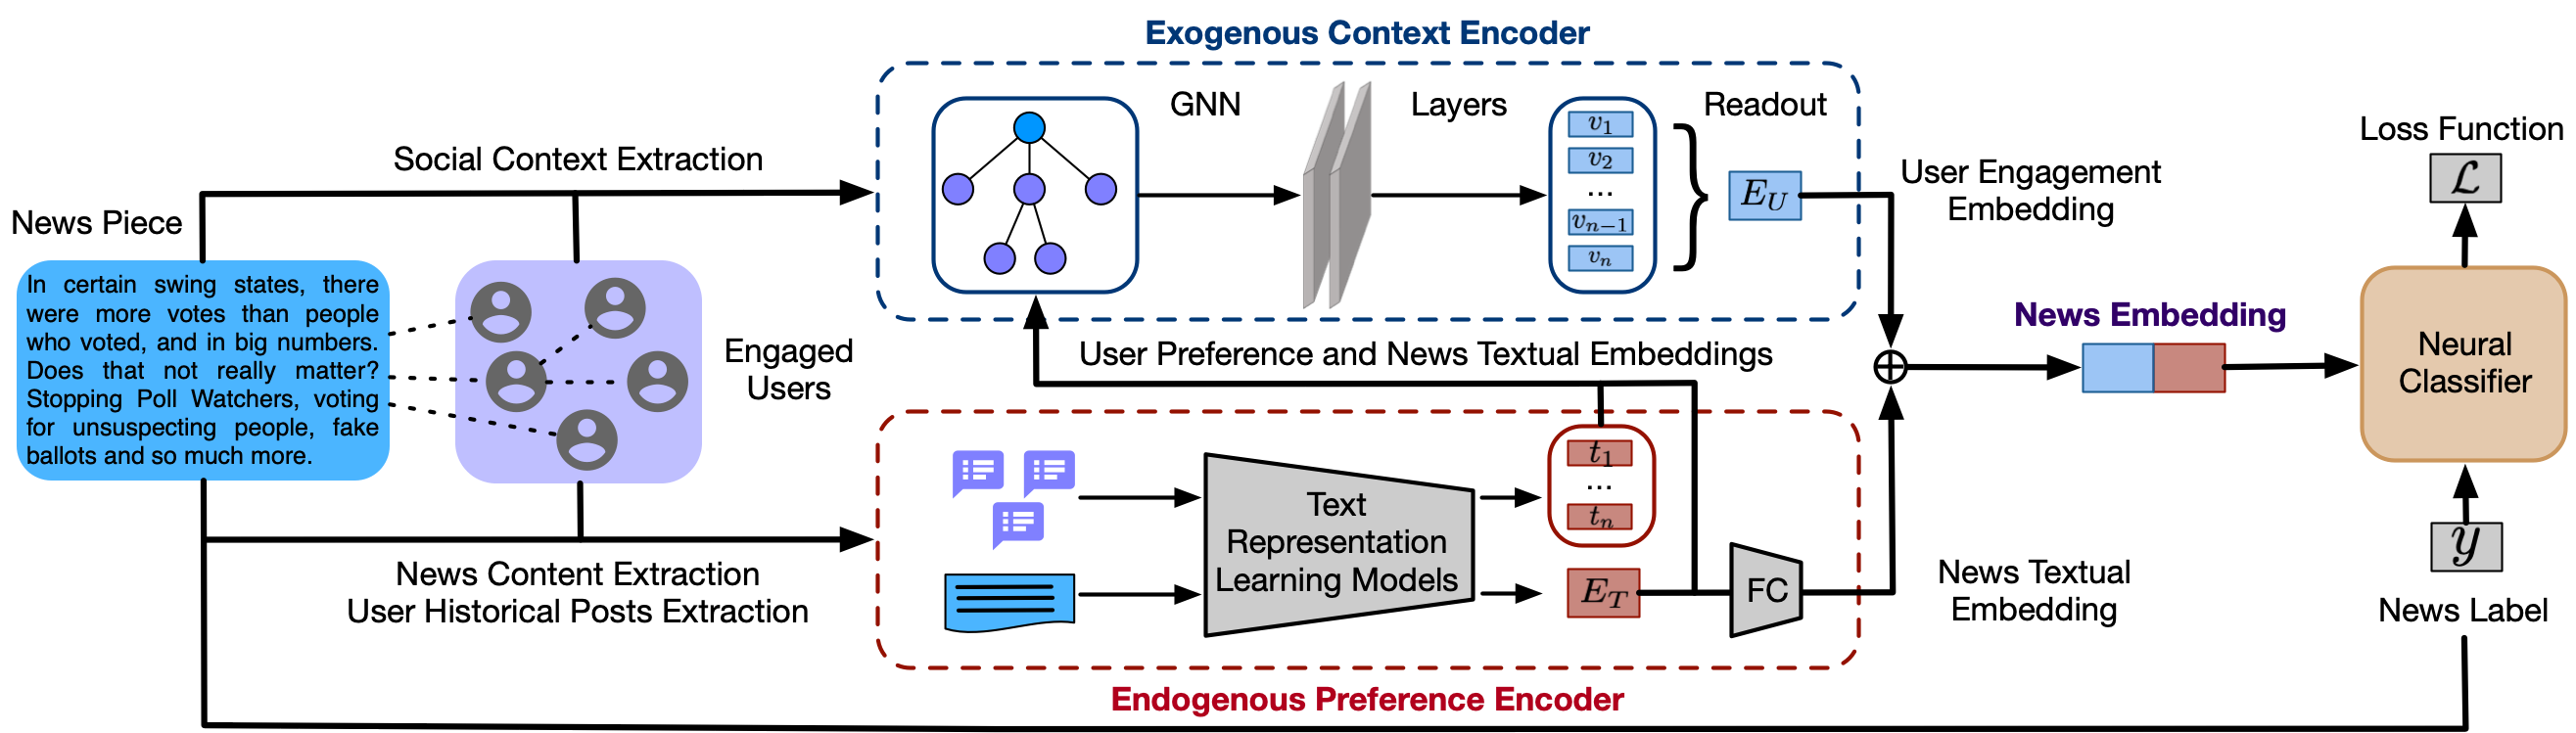
\includegraphics[scale=0.33]{UPFDFramework.png}
    \caption[UPFD Framework.]{The framework of UPFD. Figure obtained from~\parencite{UPFD_Dataset_Shu}}
    \label{fig:UPFD_Framework}
\end{figure}
\textbf{Endogenous preference encoding} deals with users' historical posts and news content using the news content and social engagement data in FakeNewsNet. With social engagement data, the authors collect 200 historical tweets of each user who have retweeted the news in FakeNewsNet. Summing up to almost 20 million tweets, this collection procedure of historical tweets for each FakeNewsNet news instance is as follows~\parencite{UPFD_Dataset_Shu}:
\begin{itemize}
    \item Collect user ids who have retweeted.
    \item For each user, collect the 200 most recent tweets.
    \item For inaccessible (suspended or deleted) users, use randomly sampled tweets from accessible users who engage in the same news piece. This step also increases the effectiveness of the exogenous encoder.
    \item  Finally, remove special characters such as "@" and URLs before applying textual techniques.
\end{itemize}
Now that we have news content and users' historical information, we encode these texts using text representation learning techniques. Still following~\cite{UPFD_Dataset_Shu}, the authors define two different settings for creating endogenous preference encoding. The first setting, \emph{spacy}, deals with obtaining the representation of users' historical data and news content with spaCy~\parencite{SpaCy_Honnibal} pretrained 300-dimensional vectors for 680K words. For each user's historical post (and similarly for each news piece), if a word appears in the text, we include the vector for that word for the final calculation in which all included vectors are averaged. As a result, we obtain a 300-dimensional vector for each user's historical information and news piece. The second setting, \emph{bert}, uses the BERT-Large model to encode news and historical user data. Using bert-as-a-service~\parencite{BertAsAService_Xiao}, the authors encode the news content with a maximum input sequence length of 768. The authors opt for a different setting to encode historical information since 200 tweets cannot be processed as a single document due to BERT's maximum input sequence length limitation of 768. It is important to note that the paper of UPFD~\parencite{UPFD_Dataset_Shu} states the maximum input sequence length as 512. However, in the dataset itself, the maximum sequence length is 768~\parencite{UPFD_PyGTeam}. Keeping in mind that tweets are usually short texts compared to news pieces, the authors use a maximum input sequence length of 16 for each historical tweet, then average all 200 tweets to obtain the final representation of users' historical data. This representation is of the same dimension as the root news node. Note that these text representation vectors are node features of a hierarchical tree-structured graph whose root node represents the news content, and the children of the root node represent the users who have retweeted.\\
\textbf{Exogenous context extraction} uses retweet information to build the previously mentioned hierarchical tree. The authors adopt a similar procedure used by~\citeauthor{GraphNeuralNetworksWithContinualLearningFakeNewsDetection_Han} (\citeyear{GraphNeuralNetworksWithContinualLearningFakeNewsDetection_Han}),\citeauthor{GeometricDeepLearningOnGraphsAndManifolds_Monti} (\citeyear{GeometricDeepLearningOnGraphsAndManifolds_Monti}), and \citeauthor{HierarchicalPropagationNetworksForFND_Shu} (\citeyear{HierarchicalPropagationNetworksForFND_Shu}). In detail, the authors define a news piece as $v_1$ and the set of users who retweeted $v_1$ as $\{v_2, \dots , v_n\}$ ordered by time. The rules are defined for this process to cover edge cases as well:
\begin{itemize}
    \item Estimate that a news piece propagates to user $v_i$ from user $v_j$ with the latest timestamp if any user from the set $\{v_j | j\in \{2, \dots, n\}\setminus \{i\}\}$ retweeted the news piece before the user $v_i$. This conservative assumption is based on the fact that the latest tweets are presented to the user first in the Twitter app~\parencite{UPFD_Dataset_Shu}.
    \item If user $v_i$ does not follow any users in the set $\{v_1, \dots, v_n \} \setminus {i}$, i.e., all retweeters and the news source except the user itself, the authors approximate the spreader of that news piece to the user $v_i$ as the user with most followers in the set. This approximation is based on the phenomenon that the tweets from accounts with more followers have a higher probability of being retweeted or viewed.
\end{itemize}
After this procedure, we have our hierarchical tree for each piece of news obtained from FakeNewsNet, which employs two sources: Politifact and Gossipcop. Thus, we evaluate these datasets separately within UPFD. The distribution of the instances with respect to train/validation/test split and label is provided in Fig.~\ref{fig:UPFD_Dataset_Visualization}.\\
\begin{figure}
    \subfloat[UPFD-Gossipcop]{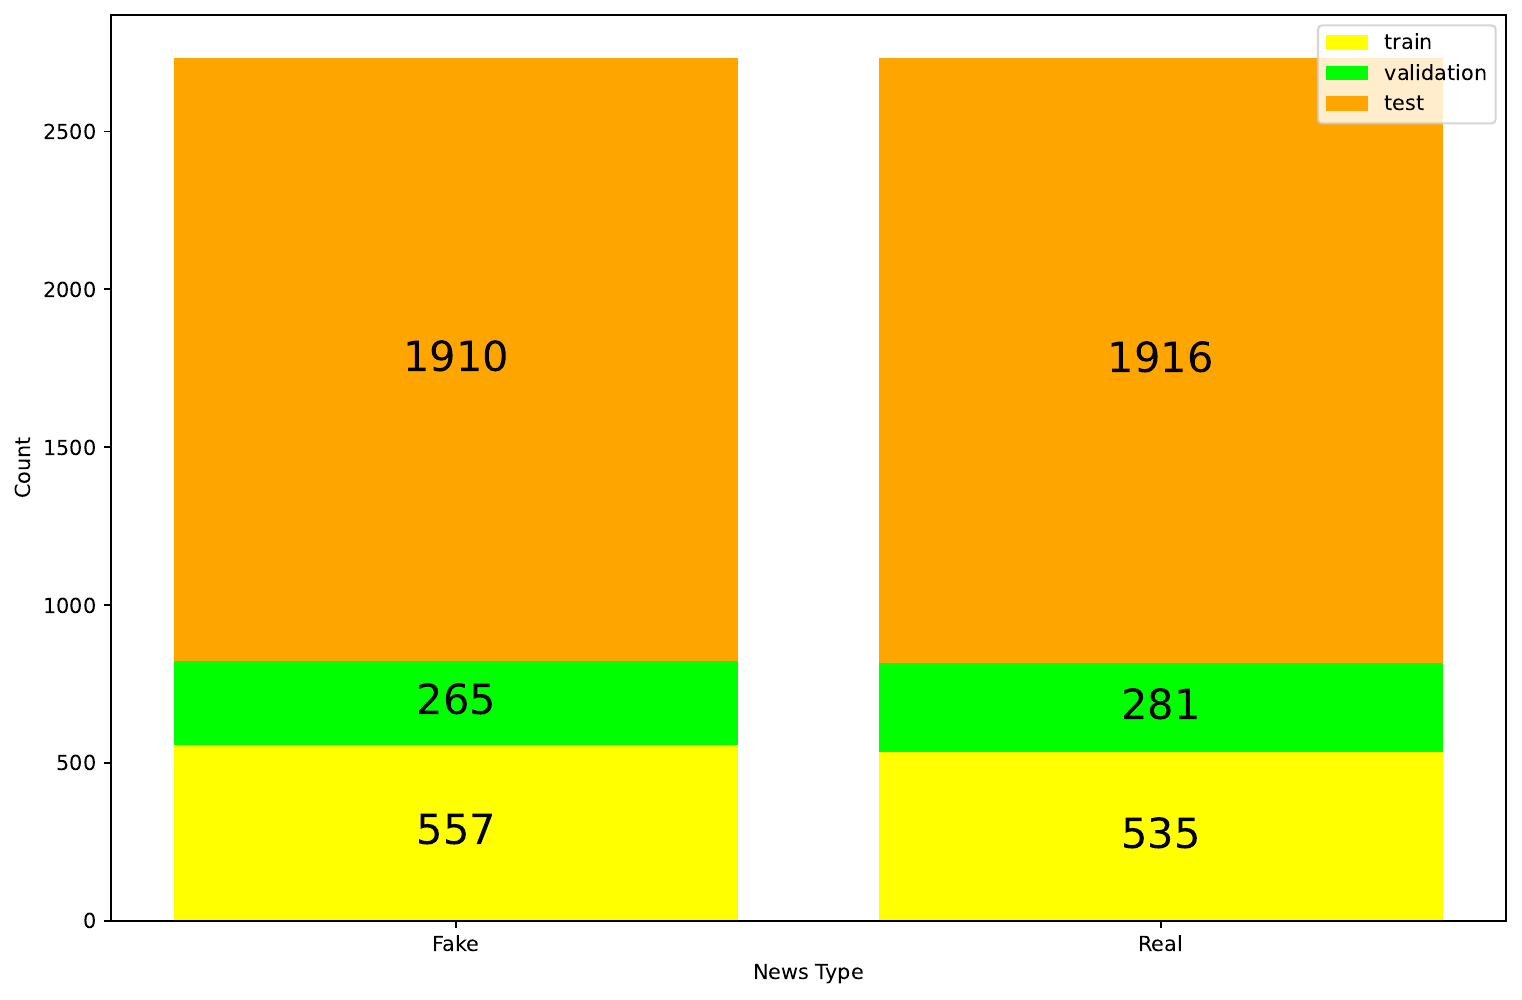
\includegraphics[width=0.45\textwidth]{GOS_DatasetDistrByLabelAndSplit.png}}
    \hfill
    \subfloat[UPFD-Politifact]{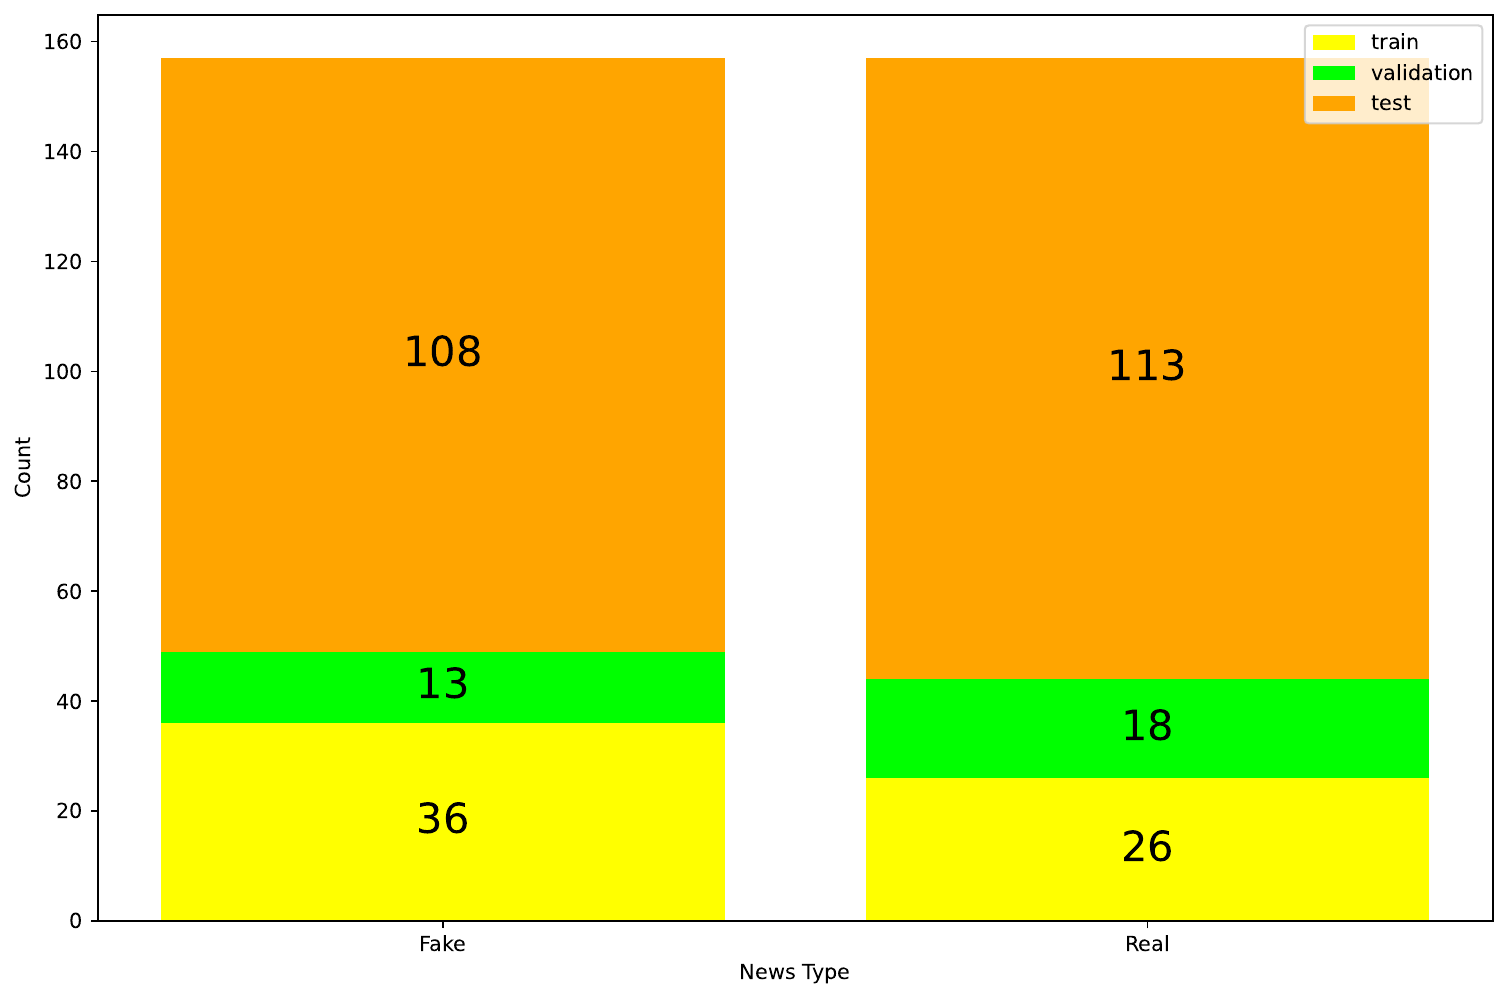
\includegraphics[width=0.45\textwidth]{POL_DatasetDistrByLabelAndSplit.png}}
    \caption[UPFD dataset distribution by label and split.]{UPFD dataset distribution by label and split (train: 20\%, val: 10\%, test: 70\%).}
    \label{fig:UPFD_Dataset_Visualization}
\end{figure}
\textbf{Information fusion} is achieved via GNNs. As discussed in~\ref{subsec:mixedApproaches_GraphNeuralNetworks}, GNNs can encode graphs by maintaining the node features and structural information. From this point on, we need to utilize the models we introduced with a classification setting. Classification is done for each graph representing the diffusion tree of the news piece~\parencite{UPFD_Dataset_Shu}. We adopted two models from this work's ablation study, the first one is based on GraphSAGE~\parencite{GraphSAGE_Hamilton}, and classification is handled with an FCN. We use BERT as the encoder since the best performance is obtained via that, according to the experiments by~\citeauthor{UPFD_Dataset_Shu} (\citeyear{UPFD_Dataset_Shu}) and the experiments we conducted. We call this model the UPFD classifier. It is illustrated in Fig~\ref{fig:UPFDClassifierArchitecture}.\\
\begin{figure}
    \centering
    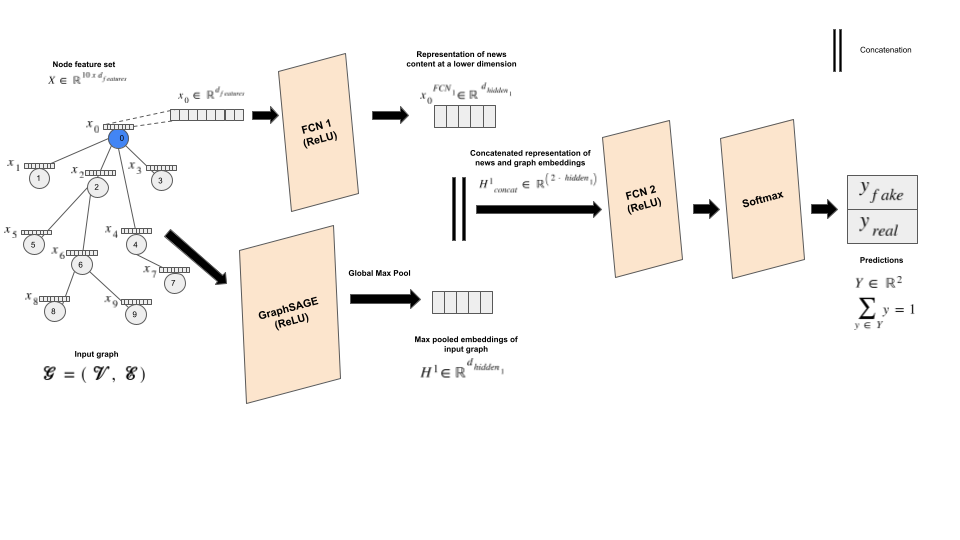
\includegraphics[scale=0.43]{UPFDClassifierArchitecture}
    \caption[The UPFD classifier model pipeline.]{The UPFD classifier model pipeline. We used an example input graph with 10 nodes. $d_{hidden_1} = 128$ stands for hidden layer dimension of FCN 1, accordingly, $d_{hidden_2} = 128$ for the hidden dimension of FCN 2, and $d_{features} = 768$ for feature dimension.}
    \label{fig:UPFDClassifierArchitecture}
\end{figure}
After obtaining the graph encodings, the authors suggest concatenating a representation of news content with graph embeddings. More precisely, the feature vector of the root node is fed to an FCN to obtain a lower-dimensional representation which is then concatenated with graph embeddings. The concatenated vector is then fed to another FCN and the softmax layer for classification. With the setting illustrated in Fig~\ref{fig:UPFDClassifierArchitecture}, the optimizer as Adam with default $\beta_1$ and $\beta_2$ and hyperparameters provided in Table~\ref{tab:UPFDClassifier_Hyperparameters}, we obtain 95.49\% and 83.16\% accuracy from the UPFD-Gossipcop and UPFD-Politifact datasets, averaged by ten runs, respectively. All other statistics are provided in Table~\ref{tab:UPFDClassifier_Results}.\\
\begin{table}
    \centering
    \begin{tabular}{|l|l|}
        \hline
        Activation function & ReLU~\parencite{ReLU_Nair} \\
        \hline
        Batch size          & 128                        \\
        \hline
        Epochs              & 35                         \\
        \hline
        Learning rate       & 0.01                       \\
        \hline
        Hidden layer 1 size & 128                        \\
        \hline
        Hidden layer 2 size & 128                        \\
        \hline
        Weight decay        & 0.01                       \\
        \hline
    \end{tabular}
    \caption[Hyperparameters of the UPFD classifier.]{Hyperparameters of the UPFD classifier.}
    \label{tab:UPFDClassifier_Hyperparameters}
\end{table}
\begin{table}
    \centering
    \begin{tabular}{c | c | c | c | c}
        \textbf{Dataset} & \textbf{Accuracy} & \textbf{Precision} & \textbf{Recall} & \textbf{F1 score} \\
        \hline
        UPFD-Gossipcop   & 95.49\%           & 94.95\%            & 96.17\%         & 95.50\%           \\
        \hline
        UPFD-Politifact  & 83.16\%           & 84.05\%            & 82.19\%         & 83.25\%           \\
    \end{tabular}
    \caption[The UPFD classifier performance metrics averaged over 10 runs.]{The UPFD classifier performance metrics averaged over 10 runs.}
    \label{tab:UPFDClassifier_Results}
\end{table}
From the model architecture, we can easily see that the UPFD classifier's social context part is propagation-based and utilize a homogeneous network. On the other hand, the news content part is unknown, but it can be uncovered using explanation techniques for GNNs. Before we explain the UPFD classifier, we outline the features of UPFD.\\
To recap, the UPFD is constructed with the news pieces and social context data obtained from FakeNewsNet~\parencite{FakeNewsNet_Shu}. \citeauthor{HierarchicalPropagationNetworksForFND_Shu} (\citeyear{HierarchicalPropagationNetworksForFND_Shu}) utilize the data from FakeNewsNet to create two levels of propagation networks: \emph{macro-level} and \emph{micro-level}. For each level,~\citeauthor{HierarchicalPropagationNetworksForFND_Shu} (\citeyear{HierarchicalPropagationNetworksForFND_Shu}) define and statistically test the significance of a set of features. We want to see if some of those features are adopted by the UPFD classifier. Briefly, macro-level networks are constructed to track the diffusion of a news piece via retweets, whereas micro-level propagation networks are built using replies to retweets. UPFD is the macro-level propagation network. Thus our focus is on the features of the macro-level propagation network.\\
The features are macro-level propagation networks are categorized into two: \emph{structural} and \emph{temporal}. Structural features capture the patterns in the global dissemination of a news piece~\parencite{HierarchicalPropagationNetworksForFND_Shu}. These features include:
\begin{itemize}
    \item ($SF_1$) \emph{Tree Depth}: Indicates how far the news piece has spread through the propagation network~\parencite{HierarchicalPropagationNetworksForFND_Shu}.
    \item ($SF_2$) \emph{Number of nodes in macro-network}: Indicates how many users have shared the news piece~\parencite{HierarchicalPropagationNetworksForFND_Shu}.
    \item ($SF_3$) \emph{Maximum outdegree}: Helps reveal the tweet/retweet with the most influence in the propagation network~\parencite{HierarchicalPropagationNetworksForFND_Shu}.
    \item ($SF_4$) \emph{Number of cascades}: The number of tweets that post the original news article~\parencite{HierarchicalPropagationNetworksForFND_Shu}.
    \item ($SF_5$) \emph{Depth of node with maximum outdegree}: Indicates steps of propagation required for a news piece to be retweeted by an influential user (node) whose post is retweeted by more users than any other users' retweet~\parencite{HierarchicalPropagationNetworksForFND_Shu}.
    \item ($SF_6$) \emph{Number of cascades with retweets}: Indicates the number of tweets that shared the original news article and retweeted at least once~\parencite{HierarchicalPropagationNetworksForFND_Shu}.
    \item ($SF_7$) \emph{Fraction of cascades with retweets}: Corresponds to $SF_6 / SF_4$~\parencite{HierarchicalPropagationNetworksForFND_Shu}.
    \item ($SF_8$) \emph{Number of bot users retweeting}: Captures the number of bot users that retweeted that news piece~\parencite{HierarchicalPropagationNetworksForFND_Shu}.
    \item ($SF_9$) \emph{Fraction of bot users retweeting}: Corresponds to $SF_8 / SF_2$~\parencite{HierarchicalPropagationNetworksForFND_Shu}.
\end{itemize}
First of all, the feature set is not restricted to these features. One can derive more features from this dataset. We
will investigate some of these features in order to understand whether we can capture similar features in our explanations.
We do not have access to the information of bot users in UPFD. Thus we drop the analysis of features $SF_8$ and $SF_9$. In addition, we did not analyze temporal features, as obtaining them from the explanation proved to be a long process. We now discuss which features' average values are found to be significant in the statistical tests conducted by~\citeauthor{HierarchicalPropagationNetworksForFND_Shu} (\citeyear{HierarchicalPropagationNetworksForFND_Shu}).\\
The first structural feature $SF_1$ is found to be consistently different for real and fake news instances in both datasets, under the statistical t-test~\parencite{HierarchicalPropagationNetworksForFND_Shu}. Concretely, this finding indicates that the tree depth of the fake news pieces is larger than that of real news pieces. Next, another simple feature $SF_2$ is also shown to be consistently different. Fake news instances have fewer nodes than real news instances. Although helpful, without additional information, this feature is too broad. Thus, we look at the next structural feature $SF_3$. It is found by~\citeauthor{HierarchicalPropagationNetworksForFND_Shu} (\citeyear{HierarchicalPropagationNetworksForFND_Shu}) that this feature is consistently different for fake and real news in Gossipcop under t-test. More precisely, it is found that the maximum outdegree is bigger in fake news instances of Gossipcop. Considering this observation, we now proceed to more complex features.\\
When we look at features that analyze more subtle properties of the dataset, such as $SF_5$ and $SF_7$, it is reported that these features are also consistently different for fake and real news instances from both datasets~\parencite{HierarchicalPropagationNetworksForFND_Shu}. According to the study, $SF_5$ is discovered to be deeper for fake news instances. The other feature $SF_7$ investigates how many of the first retweeters of the original post were retweeted. The t-test tells us that this value is different in real and fake news instances in both datasets. Specifically, the value of $SF_7$ is higher for fake news than for real news.\\
We have introduced the dataset and the model we have employed for FND in mixed approaches. We will analyze the model's behavior on the dataset. We adopt GNNExplainer~\parencite{GNNExplainer_Ying} as our explanation tool and try to uncover the patterns the model has learned. We shall also discuss some limitations we encountered while conducting these experiments.

\section{Explaining Graph Neural Networks}
\label{sec:ExplainingGNNs}
Except for GNNs, many neural networks can be explained using various tools, such as SHAP, LIME, and LRP, to name the most common ones. GNNs make their predictions by aggregating information from nodes, edges, and graph topology. There can be cases where an edge plays a significant role in the node prediction only if it is considered with another edge~\parencite{CNNsOnGraphsForLearningMolecularFingerprints_Duvenaud}. Therefore, we can not model separate contributions of node,
edge, and graph features in a linear manner.\\

\subsection{GNNExplainer}
\label{subsec:ExplainingGNNs_GNNExplainer}
GNNExplainer is a post-hoc model-agnostic explainer tool that aims to provide information about the effects of node features, edges, and graph structure on the prediction. More precisely, let us denote the node $v$'s computation graph as $\mathcal{G}_c(v)$, the binary adjacency matrix as $\mathcal{A}_c(v) \in \{0, 1\}^{n \times n}$ with $n$: the number of nodes, and the feature set as $X_c(v) = \{x_j|v_j \in \mathcal{G}_c(v)\}$. Then we say that a GNN model $f$ learns a conditional distribution $P_f(Y | \mathcal{G}_c, X_c)$ with $Y \in \{1, \dots, C\}$ as a random variable that stands for class probabilities of nodes. Then in probabilistic terms, the prediction is denoted as $\hat{y} = f(\mathcal{G}_c(v), X_c(v))$, which suggests that the prediction depends on three parts. Therefore, GNNExplainer takes into account the GNN model $f$, the graph information $\mathcal{G}_c(v)$, and the node features $X_c(v)$~\parencite{GNNExplainer_Ying}.\\
Simply put, GNNExplainer finds a subgraph $\mathcal{G}_S(v) \in \mathcal{G}_c(v)$ and node feature subset $X_S = \{x_j | v_j \in \mathcal{G}_S\}$ that are important for a given prediction $\hat{y}$. The subgraph that explains the prediction best is obtained by maximizing the \emph{mutual information} $MI$ between the prediction $Y$ and the pair of subgraph and subset of node features $(\mathcal{G}_S, X_S)$~\parencite{GNNExplainer_Ying}.
\begin{center}
    $\max\limits_{\mathcal{G}_S} MI(Y, \mathcal{G}_S, X_S) = H(Y) - H(Y|G=\mathcal{G}_S, X=X_S)$
\end{center}
where $H(Y)$ is the marginal entropy of $Y$ and is fixed for a trained GNN, and $H(Y|G=\mathcal{G}_S, X=X_S)$ stands for the conditional entropy. Since $H(Y)$ is fixed, the authors reformulate the objective function as a minimization function that looks for a subgraph $\mathcal{G}_S$ that minimizes the uncertainty of the GNN model $f$ while using a subset of node features $X_S$, thus maximizing the probability of $\hat{y}$. However, this formulation brings computation issues as large dense graphs can have massive amounts of candidate explaining subgraphs for a prediction $\hat{y}$. Thus, the authors enforce a constraint on the fractional adjacency matrix $A_S \in [0, 1]^{n \times n}$ of the subgraphs, which are now treated as random variables $\mathcal{G}_S \sim \mathcal{G}$. With convexity assumption and upper-bound from Jensen's inequality, the minimization problem is rewritten as~\parencite{GNNExplainer_Ying},
\begin{center}
    $\min\limits_{\mathcal{G}} = H(Y | G = \mathbb{E}_{\mathcal{G}} [\mathcal{G}_S, X = X_S])$.
\end{center}
Finally, to estimate $\mathbb{E}_{\mathcal{G}}$, the authors employ mean-field variational approximation and decompose $\mathcal{G}$ into a multivariate Bernoulli distribution. This allows estimating the expectation in terms of the mean-field approximation. Thus, obtaining $A_S$ whose $(i, j)$-th element denotes the expectation of the existence of the edge $(v_i, v_j)$. The final objective is defined as,
\begin{center}
    $\min\limits_M - \sum\limits_{c=1}^C \mathbb{1}[y = c] \;\;log(P_f (Y=y \;|\; \mathcal{G} = A_S \bigodot \sigma(M), X = X_S))$
\end{center}
where $M \in \mathbb{R}^{n \times n}$ is the mask to learn, $\bigodot$ is element-wise multiplication, and $\sigma$ is
the mapping function of the mask to values to interval $[0, 1]^{n \times n}$~\parencite{GNNExplainer_Ying}. For large graphs, however, a threshold might be required to remove low values in the mask. We will propose two approaches to effectively
handle this only for explanations of the UPFD classifier~\parencite{GNNExplainer_Ying}.\\
Besides the edge mask $M$, as mentioned previously, GNNExplainer also learns a node mask $F \in \{0, 1\}^d_{features}$ through a binary feature selector that is learned by maximizing $MI$ in the first equation. Formally, the explanation $(\mathcal{G}_S, X_S)$ is optimized together to maximize $MI$:
\begin{center}
    $\max\limits_{\mathcal{G}_S, F} \;\; MI (Y, (\mathcal{G}_S, F)) = H(Y) - H(Y \;|\; \mathcal{G} = \mathcal{G}_S,\; X = X_S^F)$
\end{center}
where $X_S^F = \{x_j^F|v_j \in \mathcal{G}_S\}$ and $x_j^F = [x_{j, t_1}, \dots, x_{j, t_k}]$ for
$F_{t_i} = 1$ denotes the node features that are not masked out by F~\parencite{GNNExplainer_Ying}. So far, the
explanation method is defined for the node classification setting. However, when the task is at the graph-level, the method needs to be extended. \citeauthor{GNNExplainer_Ying} (\citeyear{GNNExplainer_Ying}) suggest unionizing the adjacency matrices $A_S$ for all nodes in the graph to be explained. The aggregation of node embeddings, however, restricts the explanation to a subset, where the resulting subgraph must be connected. Thus, the threshold for the edge mask is set to a very low value or zero. This allows for a larger connected subgraph as an explanation~\parencite{GNNExplainer_Ying}.\\


\subsection{Explainability of UPFD Classifier}
\label{subsec:ExplaniningGNNs_ExplainingUPFDClassifier}
In Section~\ref{sec:mixedApproaches}, we have introduced the UPFD classifier, a GNN that uses GraphSAGE~\parencite{GraphSAGE_Hamilton} as the graph encoder, two FCNs, and softmax for the classification of news propagation trees. We now investigate the mixed model's behavior on the UPFD-Politifact dataset by employing GNNExplainer. Note that this model was trained only on the UPFD-Politifact dataset; thus, data in UPFD-Gossipcop is unseen to this model. The explanations we obtain for our classifier on the UPFD-Politifact dataset might provide us with useful information that allows us to understand the model's reasoning.\\
First, to clarify how the explanations should be interpreted, let us consider an example where we obtain a single explanation $(\mathcal{G}_S, X_S)$ for a news diffusion tree. We interpret the edge masks $M$ of $\mathcal{G}_S$ as the importance scores of edges between nodes. Therefore, an edge $(v_i, v_j)$ with a mask value $m_{ij}$ lower than a fixed $threshold$ will be dropped. After the $threshold$ is applied, if a node $v_i$ is not connected to the largest connected subgraph, it will not be included in the visualization of the explanation. \\
\begin{figure}
    \centering
    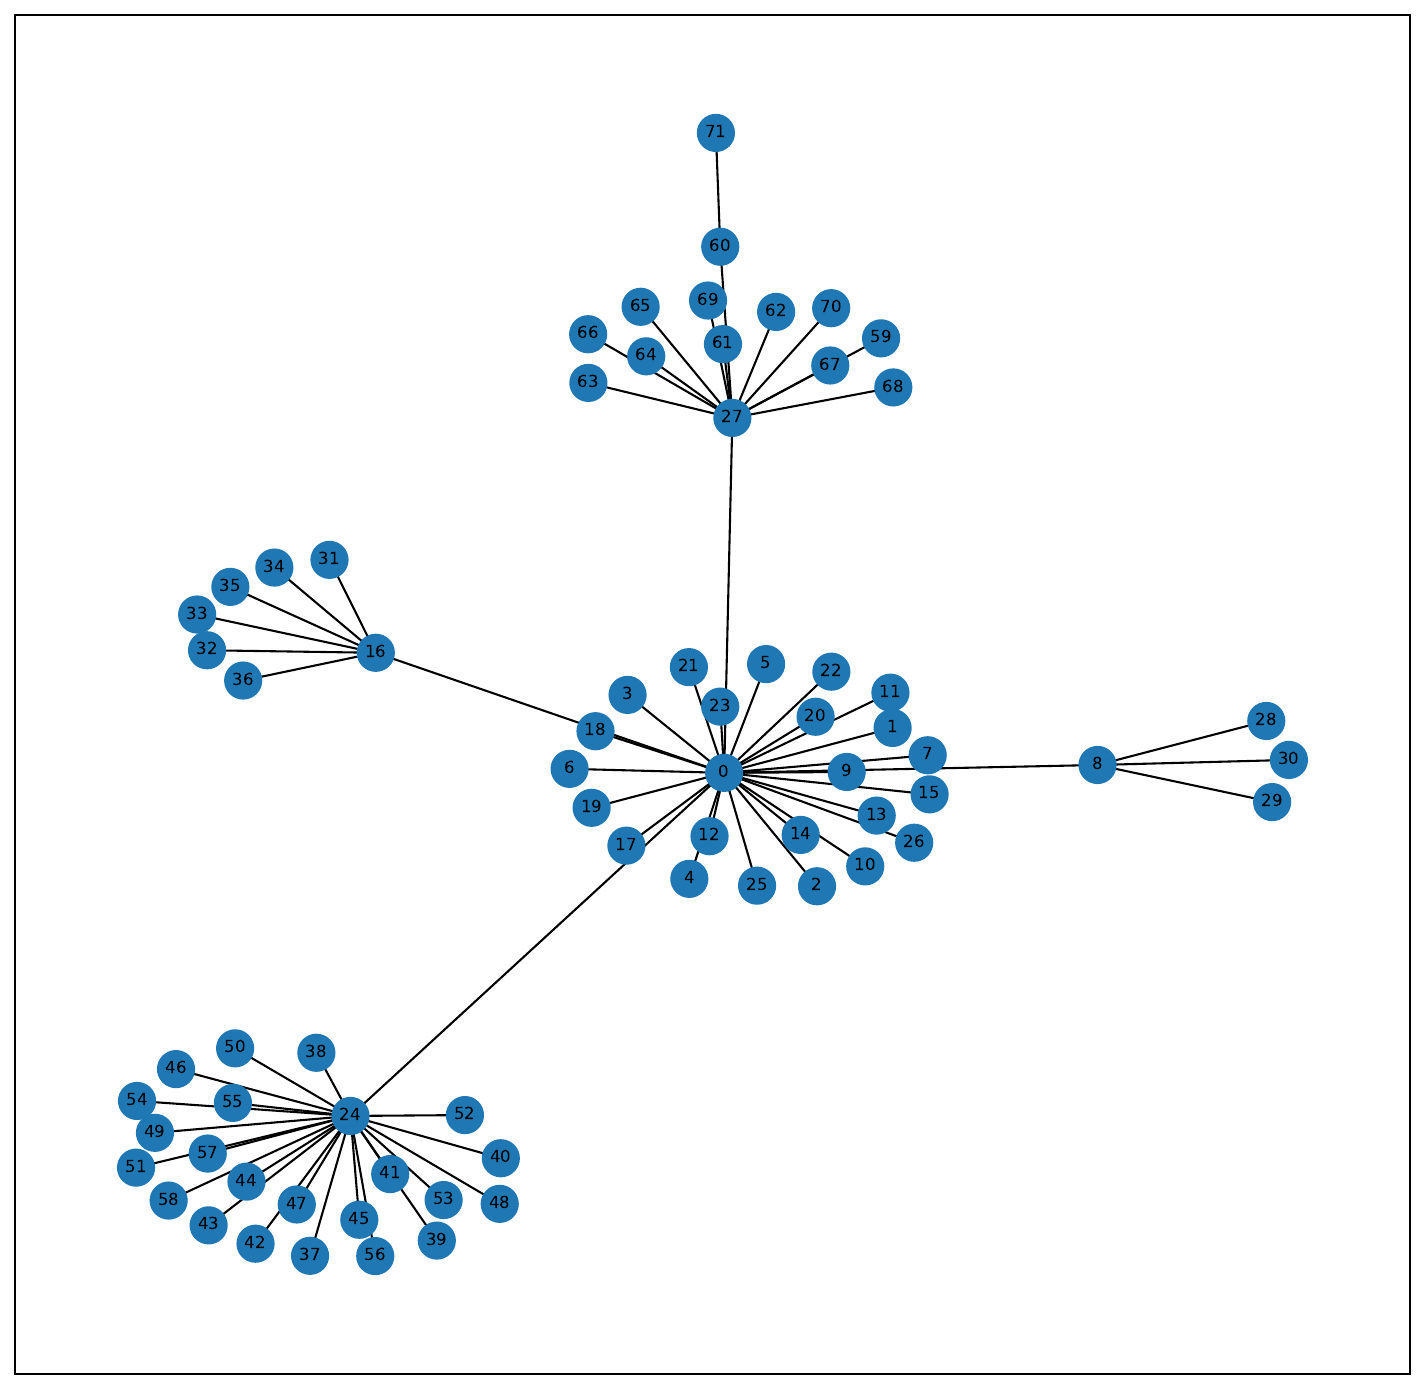
\includegraphics[scale=0.45]{EchoChamberExample1}
    \caption[Echo chamber example from the UPFD-Politifact dataset.]{A fake news instance in the UPFD-Politifact dataset that exhibits echo chamber behavior. $0$-th node represents the root node with news embeddings. We will refer to this fake news example as the \emph{echo chamber example}.}
    \label{fig:echoChamberExample1}
\end{figure}
We examine whether our classifier learned a similar intuition that we discussed in~\ref{subsec:fakeNewsDetection_fakeNews}. Recall that echo chambers are one of the significant reasons that fake news pieces spread. We analyze an example from the train split of the UPFD-Politifact dataset, some of whose cascade nodes exhibit echo chamber structures. To be precise, there is no clear definition of echo chambers in the context of diffusion trees. For the echo example in Fig.~\ref{fig:echoChamberExample1}, we assume that any cascade node with more than two child nodes, each of which do not have children, has an echo chamber.\\
In the echo chamber example in Fig.~\ref{fig:echoChamberExample1}, we observe some echo chambers created by cascade nodes $24$, $27$, $16$, and $8$ from biggest to smallest, respectively. We look for features introduced in~\ref{subsec:mixedApproaches_DatasetAndModel} that are captured by the UPFD classifier. First, let us observe the explaining subgraph $\mathcal{G}_S$ in Fig~\ref{fig:EchoChamberExample1Explanation_no_threshold} for the echo chamber example.\\
\begin{figure}
    \centering
    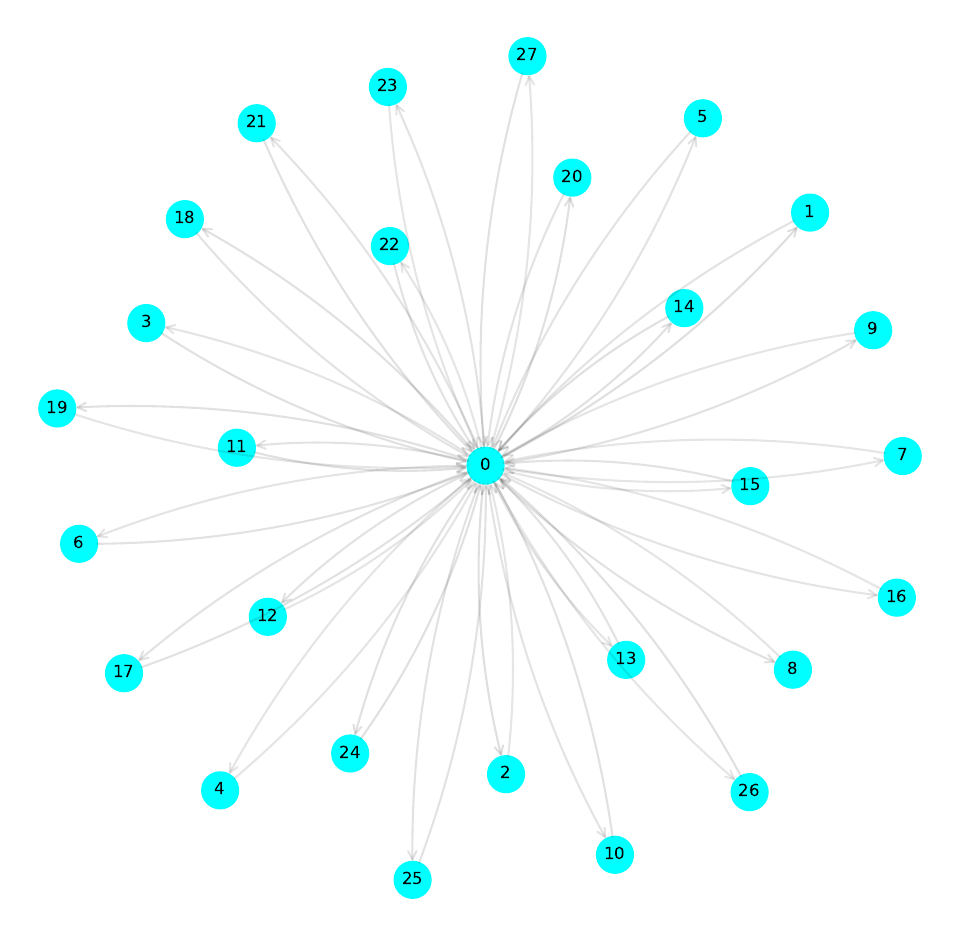
\includegraphics[scale=0.45]{EchoChamberExample1Explanation_no_threshold.png}
    \caption[Echo chamber example explanation for root node.]{The explanation provided for the UPFD classifier and the echo chamber example for its root node. This instance was predicted as fake news with a probability of $0.9912$. Contains 28 nodes.}
    \label{fig:EchoChamberExample1Explanation_no_threshold}
\end{figure}
Even though UPFD has undirected edges, we have obtained an explanation with bidirectional directed edges. Recall that undirected edges are interpreted as bidirectional edges. This is why GNNExplainer provided us with two edges per node pair. Additionally, there exist self-loops for each node, but those are not included in the visualization. Self-loops are edges from and to the same node $(v_i, v_i)$. The edge mask values for edges indicate the importance of the messages passed between two nodes. The transparency of the edges is an indicator of the magnitude of the edge mask value. However, this can not be clearly observed in this example.\\
On the other hand, when we inspect the node feature mask $F$, we can understand which features are deemed important by the UPFD classifier for a given node. We are particularly interested in the root node and the node feature mask associated with it. Since the root node consists of news content embeddings, intuitively, we can consider the root node feature mask as the importance scores of news content embeddings or tokens. However, we were not able to utilize node feature masks due to (i) the time needed to download the FakeNewsNet~\parencite{FakeNewsNet_Shu} (around 80\% was completed in over two months), whose news content and social context data were utilized in UPFD, (ii) insufficient information from~\citeauthor{UPFD_Dataset_Shu} (\citeyear{UPFD_Dataset_Shu}) to reproduce the UPFD framework, (iii) large maximum input sequence (768) for BERT model to process the news content on a local computer. Thus, we continue our analysis without considering the node feature mask. \\
\textbf{Interpreting the Explanation.} According to the explaining subgraph, the UPFD classifier thinks that the cascades are the most important nodes for the prediction of fake for this instance. If we only consider the echo chamber effect, we would expect higher edge mask values for the edges of the cascade nodes $v_8$, $v_{16}$, $v_{24}$, and $v_{27}$. Accordingly, we observe larger importance scores on edges that connect these nodes to the root node. The edge $(v_0, v_{13})$ was assigned the highest edge mask value with $0.1371$. The edges $(v_0, v_8)$, $(v_0, v_{16})$, $(v_0, v_{24})$, and $(v_0, v_{27})$ were assigned $0.1081$, $0.0951$, $0.1222$, and $0.1181$, respectively.  While the reasons behind the maximal importance score assignment to the edge $(v_0, v_{13})$ remain unclear, we observe that the biggest echo chamber's connection to the root node has a high edge mask value, which suggests that the UPFD classifier might be utilizing the echo chamber effect with success for prediction. However, we need to observe similar behaviors in other fake news instances that house echo chambers.\\
We also examined five edges with the highest edge mask values to understand which edges are important for the UPFD classifier. Before we proceed, it should be noted that the subgraph generation does not directly take into account where the maximal edge mask values reside. Instead, it tries to capture the biggest subgraph with the highest mutual information between the original graph and the subgraph with respect to the prediction. Hence, some edges we will analyze might not be in the explaining subgraph.\\
\textbf{Edge Mask Analysis.} Proceeding our analysis for the five largest values in the edge mask provided by GNNExplainer, we observed that the second highest value belongs to the edge $(v_{24}, v_{41})$, i.e., an echo chamber connection. The third one belongs to a self-loop $(v_{44}, v_{44})$, and the fourth one is for the edge $(v_{44}, v_{24})$. We can interpret the edge mask value for the self-loop as the significance that the UPFD classifier puts on node $v_{44}$. The edge mask value for edge $(v_{44}, v_{24})$ confirms our interpretation for node $v_{44}$ because this is the first instance of an important edge that is directed from a retweeter to its source. Thus, the user $v_{44}$ and their historical data should be investigated for further insights. Also, one can look for the same user in the other fake news instances to understand this user's involvement. The fifth-largest edge mask value is assigned to the edge $(v_{27}, v_{62})$, which is another propagation edge in an echo chamber. The distribution of the edge mask values is given in Fig.~\ref{fig:EchoChamber1SubgraphEdgeMaskDistribution}.\\
% \begin{figure}
%     \centering
%     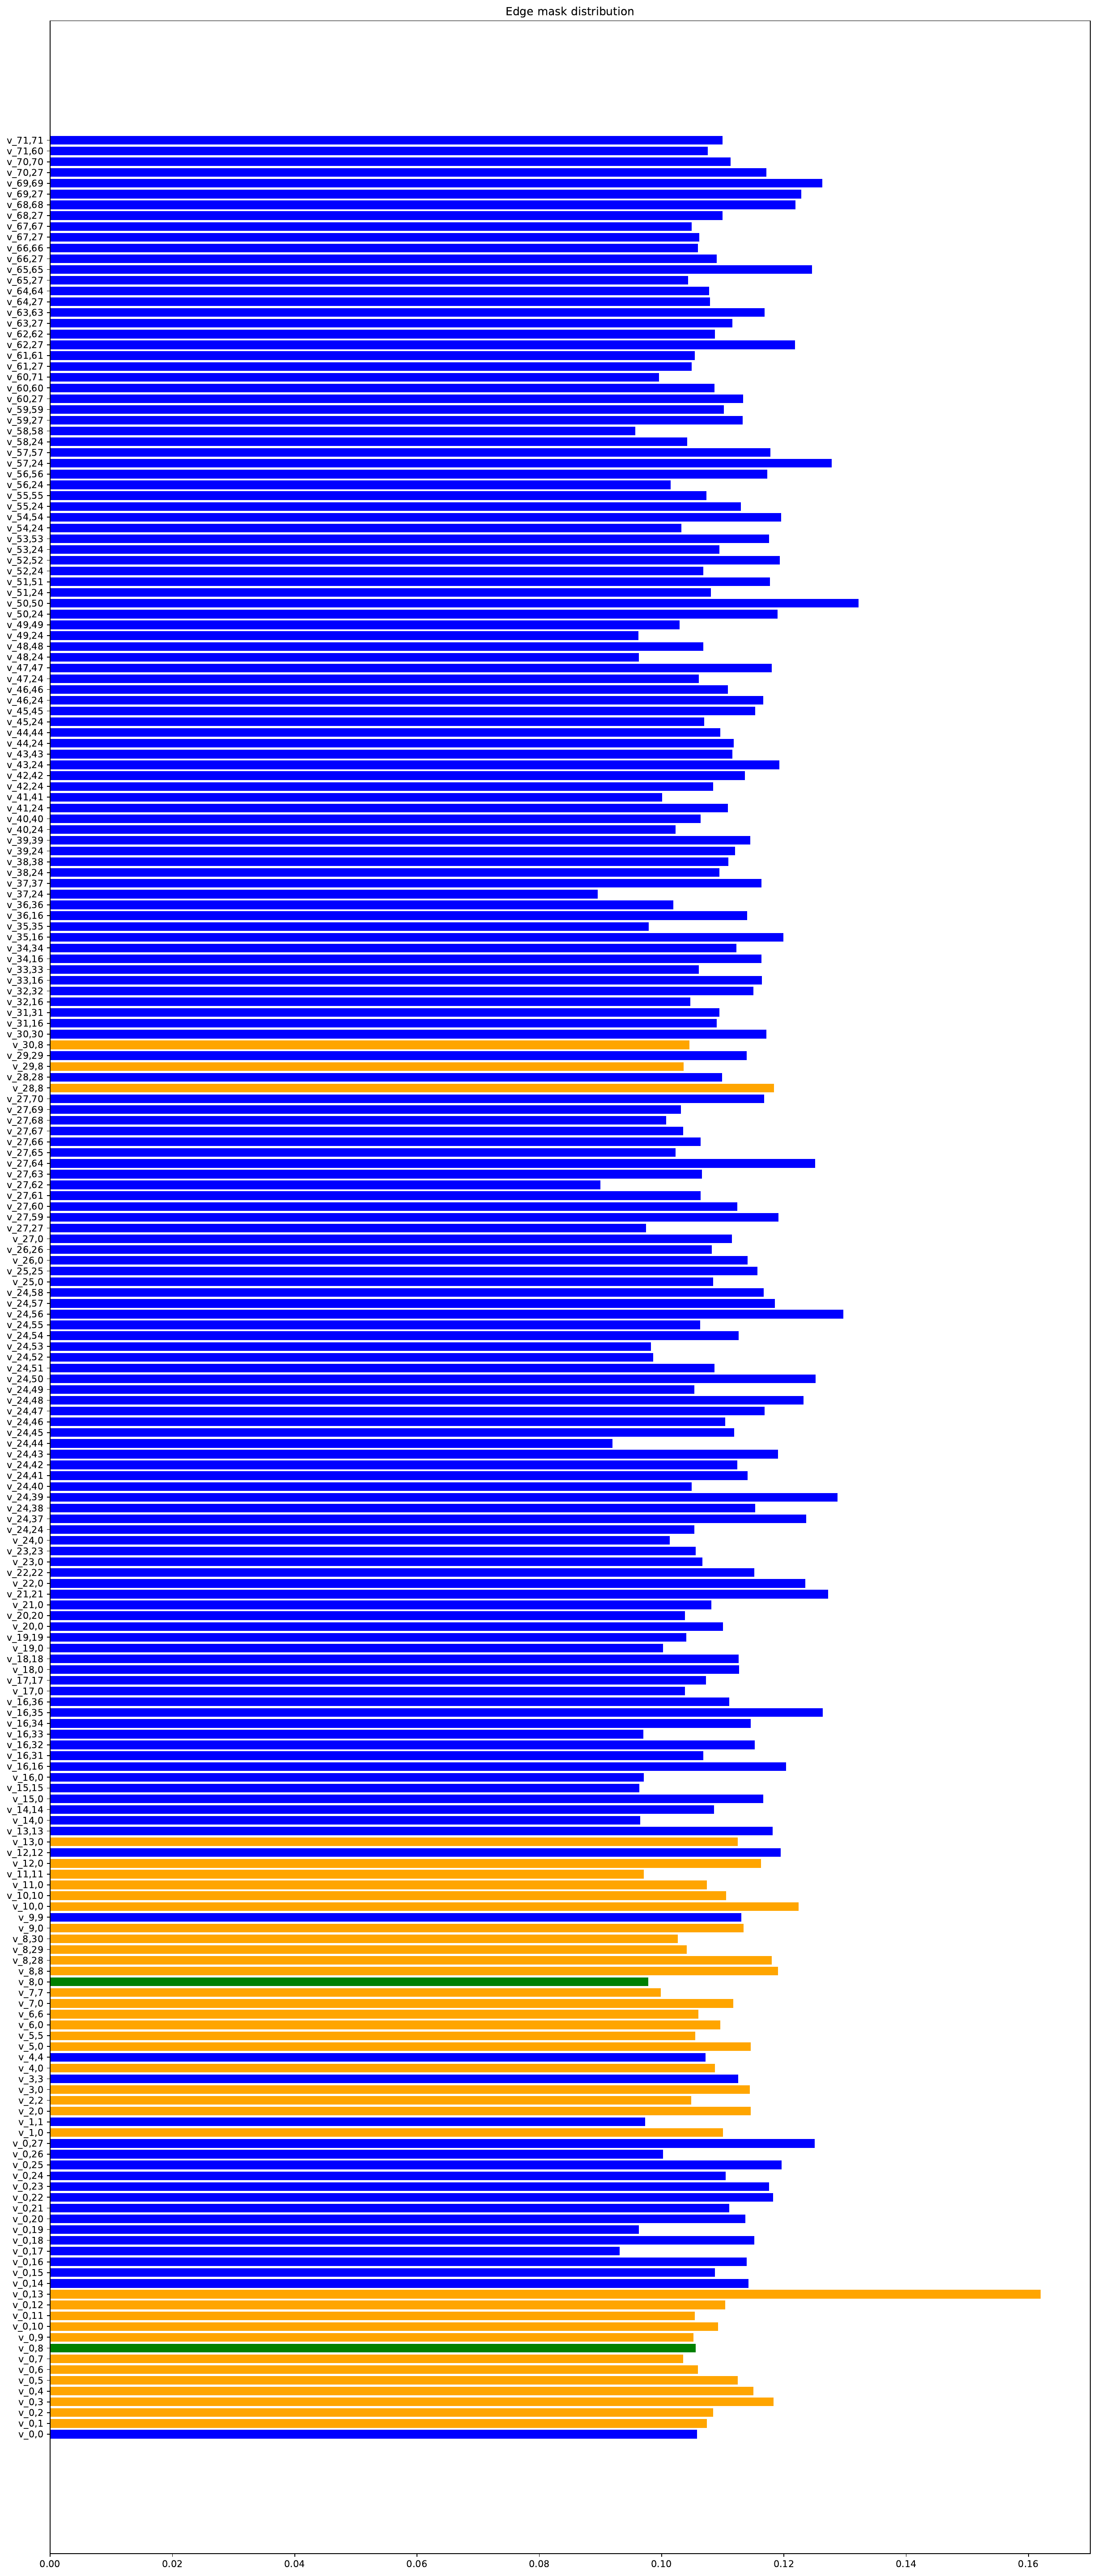
\includegraphics[scale=0.15]{EchoChamber1EdgeMaskDistribution.png}
%     \caption[Edge mask distribution of the input graph provided for echo chamber example explanation.]{Edge mask distribution of the input graph provided for echo chamber example explanation. The orange bars represent the edge mask values of the edges included in the subgraph explanation. Green bars indicate edges with the same characteristic as orange bars, but these edges are also connections to echo chambers.}
%     \label{fig:EchoChamber1EdgeMaskDistribution}
% \end{figure}
\begin{figure}
    \centering
    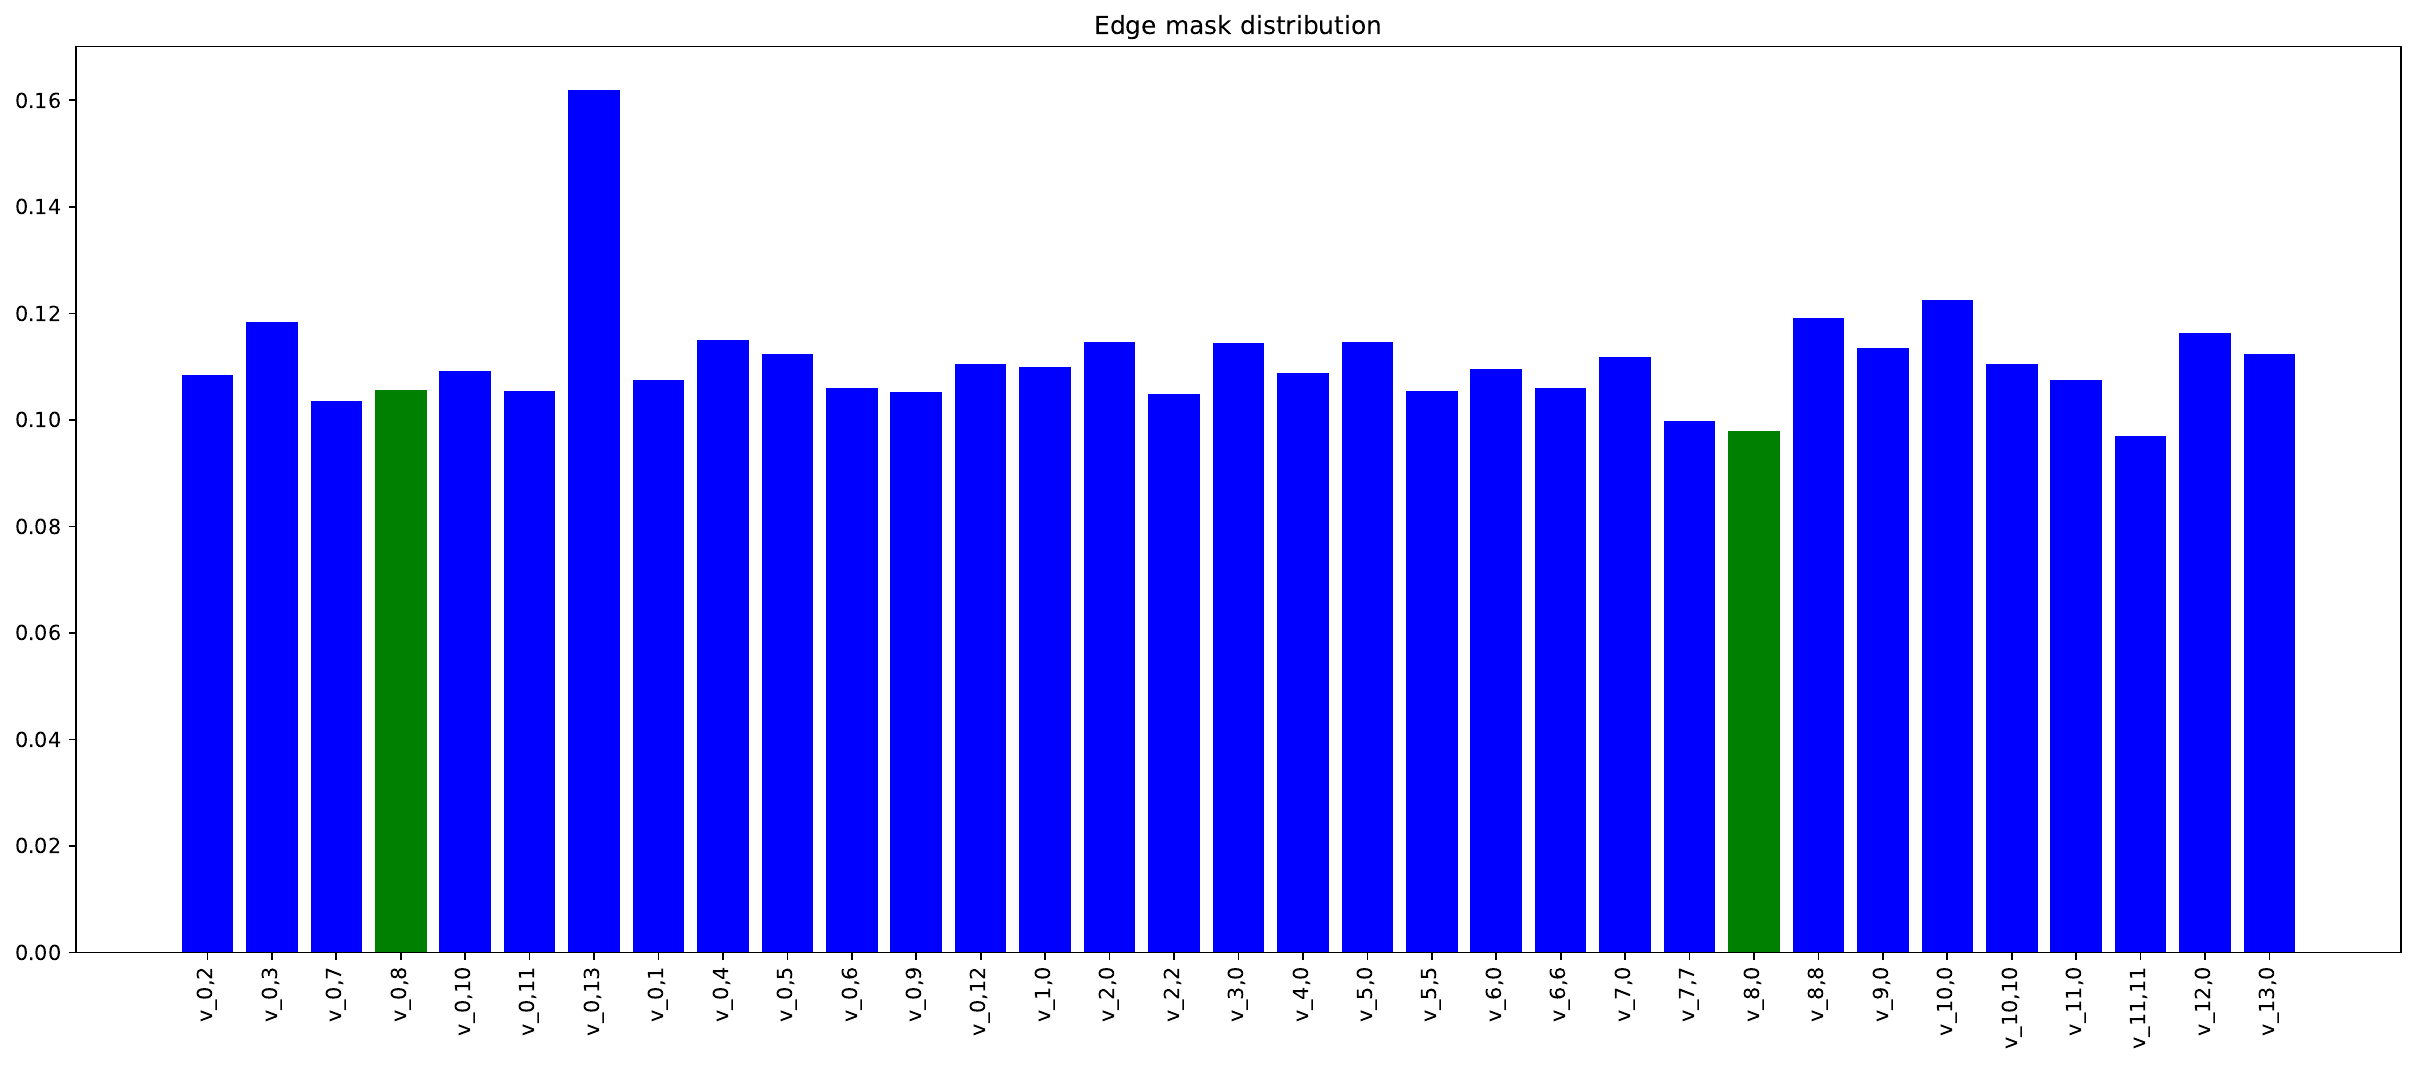
\includegraphics[scale=0.35]{EchoChamber1SubgraphEdgeMaskDistribution}
    \caption[Edge mask distribution of the subgraph provided for echo chamber example explanation.]{Edge mask distribution of the subgraph provided for echo chamber example explanation. The green bars represent the edge mask values of echo chamber connections.}
    \label{fig:EchoChamber1SubgraphEdgeMaskDistribution}
\end{figure}
Visiting back to the features we introduced, we observe that the feature $SF_7$ is captured in this explanation. To elaborate, we see that the edges to the cascade node with retweets were deemed more important by the explainer. This implies that the UPFD classifier captured an important feature for this instance. Although, this can not be clearly observed by looking at the explaining subgraph since the transparencies of the edges are not discriminative enough.\\
%Although, in order to get this interpretation, one would require a data scientist. A domain expert or an end user is likely to either misinterpret or not understand the explanation provided by GNNExplainer. Furthermore, some of the most important edges were not even included in the visualization. This certainly decreases the understandability of the explanations.\\
\textbf{The Faithfulness of Explanations.} We also analyzed the faithfulness of the explanations to the UPFD classifier. We took the explaining subgraph we provided in Fig.~\ref{fig:EchoChamberExample1Explanation_no_threshold}, restored its node features, and fed it to the UPFD classifier to see if the learned structure is still predicted as fake with high probability. In fact, the UPFD classifier predicted the subgraph as fake with $0.9915$, which is higher than the prediction probability of the original input. Overall, we say that the explaining subgraph of this instance is faithful to the UPFD classifier, and GNNExplainer can indeed reduce noise in a graph, as~\citeauthor{GNNExplainer_Ying} (\citeyear{GNNExplainer_Ying}) claim. We also observe close prediction probabilities for the original graph and the explaining subgraph in the sensitivity analysis results in Table~\ref{tab:echoChamberFeatureRemovalExperimentResults}. This further shows that this explanation is faithful for this instance.\\
\textbf{Sensitivity Analysis.} We proceed with our analysis of the echo chamber example by removing the news content and historical information of children nodes, both from the original graph and the explaining subgraph, to see their effect on the prediction. We provide the results in Table~\ref{tab:echoChamberFeatureRemovalExperimentResults}.\\
\begin{table}
    \centering
    \begin{tabular}{c | c | c}
        \textbf{Operation}            & $p_{original}$ & $p_{subgraph}$ \\
        \hline
        No change                     & 0.9912         & 0.9915         \\
        \hline
        Remove news content           & 0.8328         & 0.8018         \\
        \hline
        Remove historical information & 0.9812         & 0.9809         \\
        \hline
        Remove all node information   & 0.4940         & 0.4940         \\
    \end{tabular}
    \caption[Model prediction probabilities for input perturbation experiment.]{Model prediction probabilities for input perturbation experiment. $p_{original}$ denotes prediction probability for the original input. Analogously, $p_{subgraph}$ refers to the prediction probability for the explaining subgraph.}
    \label{tab:echoChamberFeatureRemovalExperimentResults}
\end{table}
It is trivial to observe in Table~\ref{tab:echoChamberFeatureRemovalExperimentResults} that the UPFD classifier's confidence decreases as we remove news content for the echo chamber example. Interestingly, when we remove users' historical information from all nodes except the root node, the prediction probability almost does not decrease. This suggests the UPFD classifier takes into account the news content and structural information more than the historical information. This behavior can also be observed from the UPFD classifier's architecture in Fig.~\ref{fig:UPFDClassifierArchitecture}. The skip connection and concatenation of the news content in the root node appear to be doing what is expected of it. In fact, the authors of UPFD~\parencite{UPFD_Dataset_Shu} showed that with a vanilla version of the UPFD classifier, i.e., without skip connection and concatenation, the performance drops. This finding of ours also goes in parallel with their finding. Furthermore, when we remove all node information, the UPFD classifier can no longer tell fake from real. Thus, without node information, just depending on the structure of the echo chamber example for prediction turns out to be a bad idea. We certainly need the node embeddings, at least for the news.\\
We illustrate more examples in order to understand if the statistically significant features were captured in other instances. First, it is nontrivial to look for $SF_1$ in the explanations as the tree depth will be decreased significantly. Most of the time, the tree depth in the explanations we observed was one. Thus, we skip this feature analysis. We look for the effect of feature $SF_2$ in the explanations. We compare our echo chamber example in Fig.~\ref{fig:echoChamberExample1} with a real news example in Fig.~\ref{fig:POL_RealNewsExample1}. The echo chamber example has 72 nodes, whereas the real news example has 59 nodes. Now let us observe the explanation provided for the real news instance in Fig.~\ref{fig:POL_RealNewsExample1Explanation_no_threshold}.\\
\begin{figure}
    \centering
    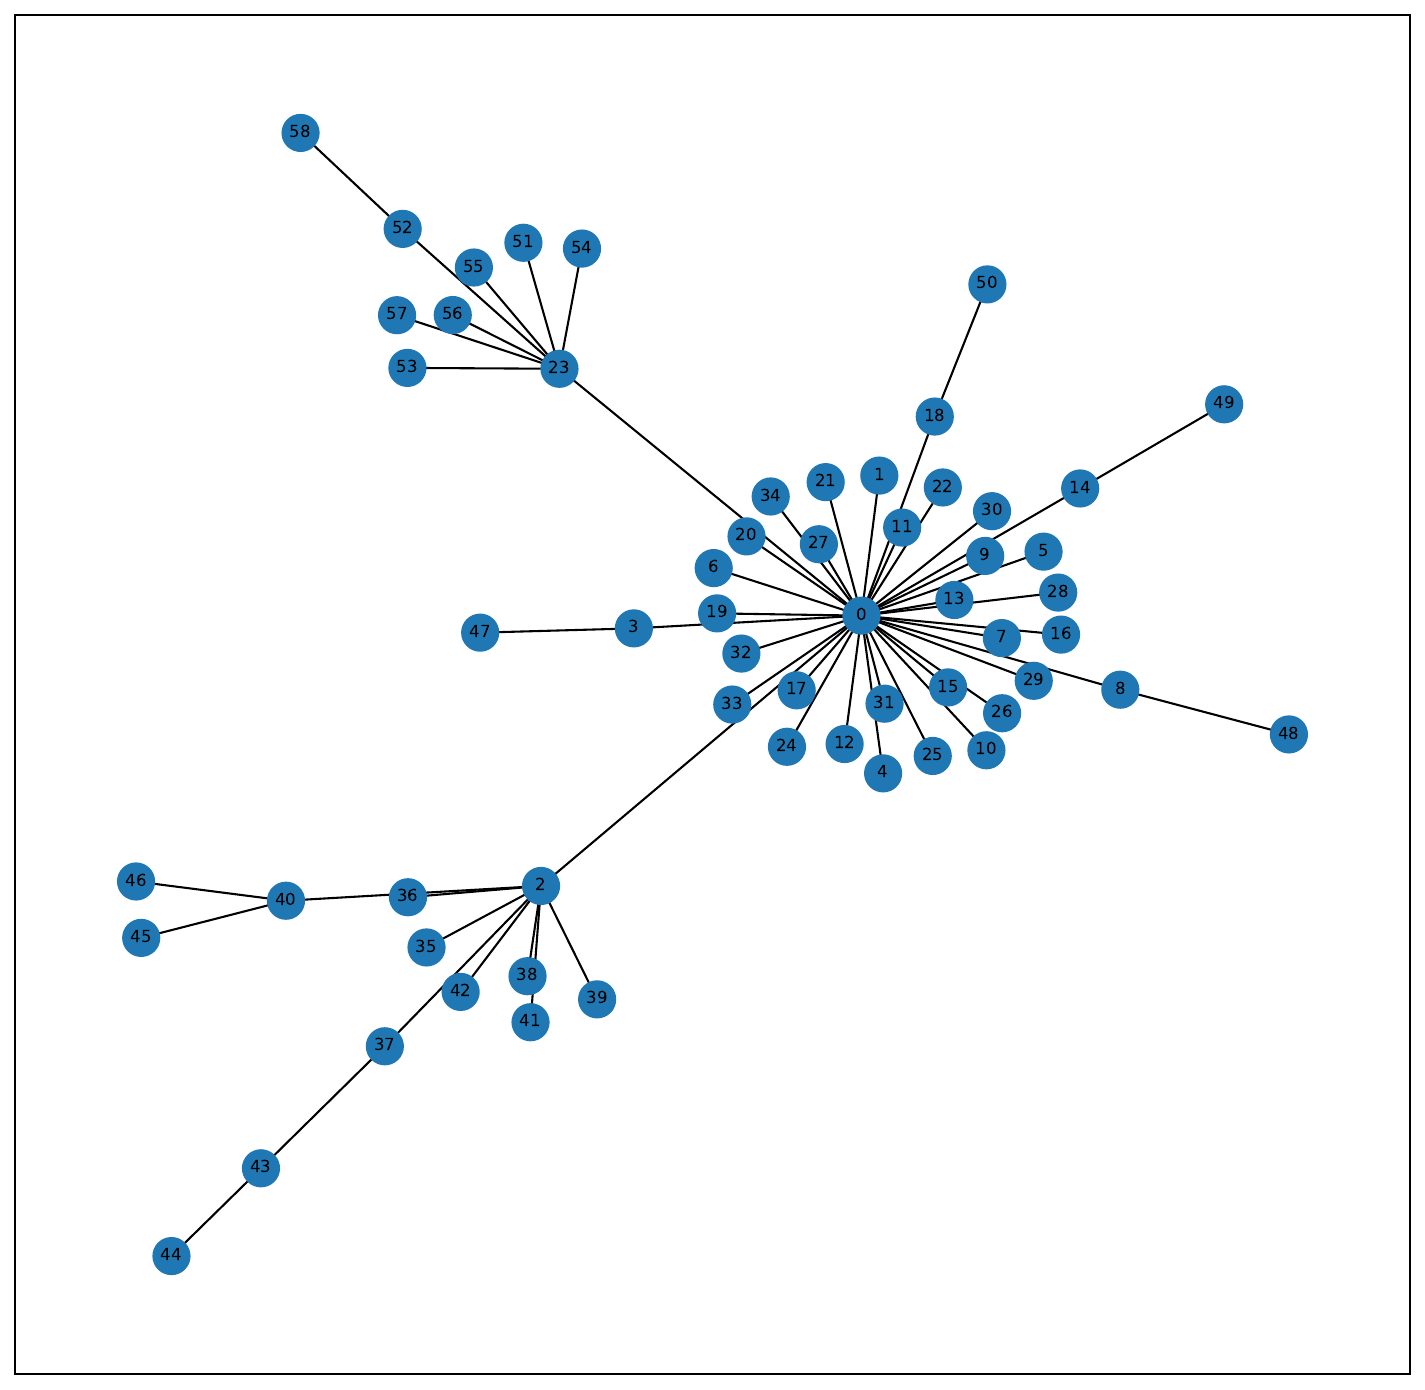
\includegraphics[scale=0.45]{POL_RealNewsExample1}
    \caption[A real news instance from UPFD-Politifact.]{A real news instance from UPFD-Politifact. We shall refer to this example as the \emph{real news example}. It was predicted as real news with probability 0.9956.}
    \label{fig:POL_RealNewsExample1}
\end{figure}
\begin{figure}
    \centering
    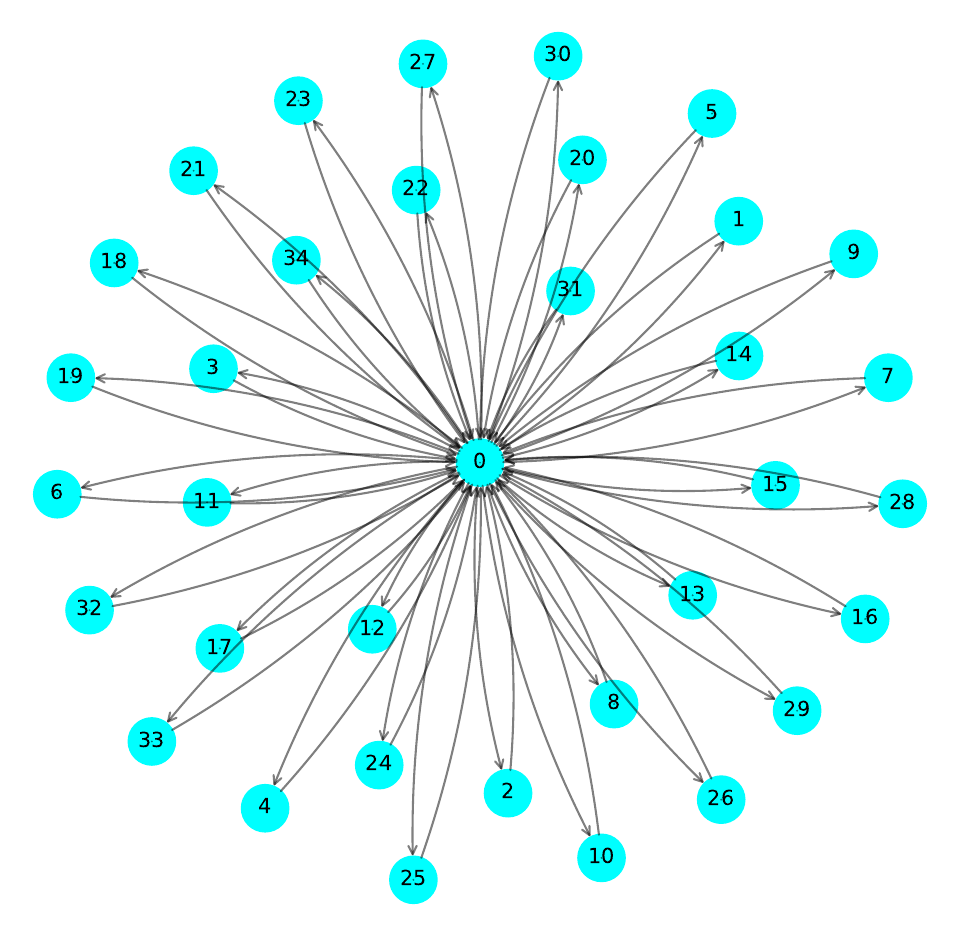
\includegraphics[scale=0.45]{POL_RealNewsExample1Explanation_no_threshold}
    \caption[Explanation of the real news example from UPFD-Politifact]{Explanation of the real news example from UPFD-Politifact. Contains 35 nodes.}
    \label{fig:POL_RealNewsExample1Explanation_no_threshold}
\end{figure}
The explaining subgraph of the real news example contains more nodes than the explaining subgraph for the echo chamber example. This might imply the effect of $SF_2$ on the explanations. In other words, explanations capture the importance of more nodes for the real news example. Although, this should be tested with other real and fake news instances to be verified. This instance has some nodes that exhibit a partial echo chamber effect. Still, we can easily observe that some of these nodes were also retweeted, a behavior not observed in the echo chamber example.\\
\textbf{Latent Space Analysis.} We apply the t-SNE~\parencite{tSNE_vanDerMaaten} function by scikit-learn~\parencite{ScikitLearn_Pedregosa} to see if GraphSAGE is able to distinguish fake and real news before its outputs are concatenated with news content in the root node and then fed to the FCN. We set the perplexity to 10, the initialization method to Principal Component Analysis (PCA), the learning rate to the \emph{auto} option, and the number of iterations to 1000, and kept the remaining parameters' default values as defined in~\cite{ScikitTSNE_scikit}. The visualization for this procedure is provided in Fig~\ref{fig:TSNE_GraphSAGE}.
\begin{figure}
    \centering
    \subfloat[UPFD-Gossipcop]{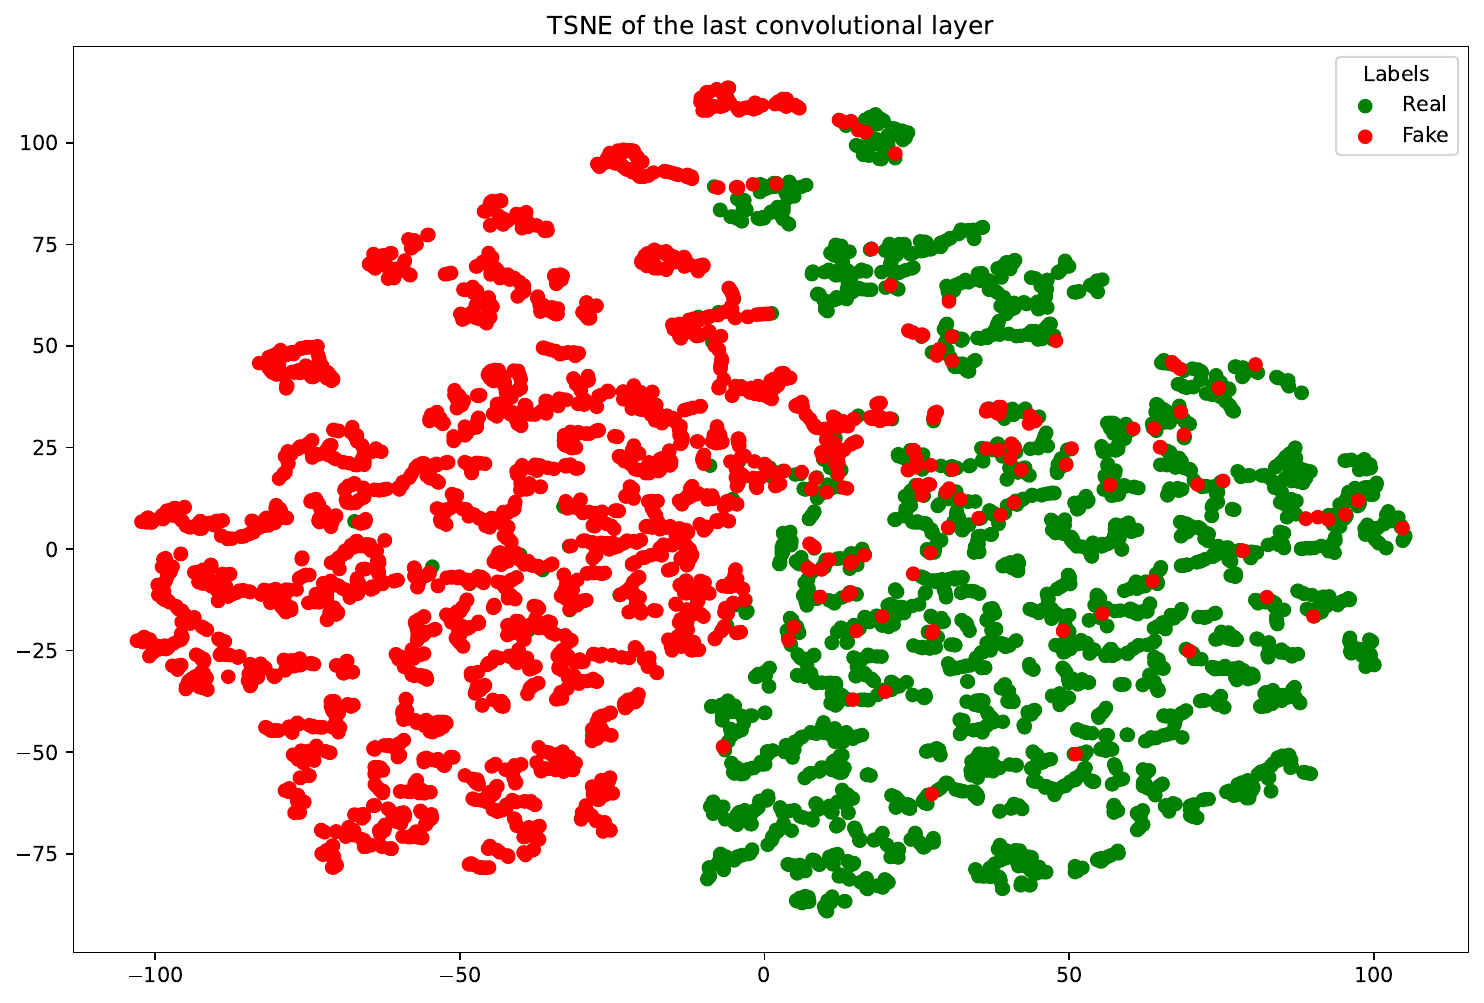
\includegraphics[width=0.45\textwidth]{TSNE_GraphSAGE_GOS.png}\label{subfig:TSNE_GraphSAGE_GOS}}
    \hfill
    \subfloat[UPFD-Politifact]{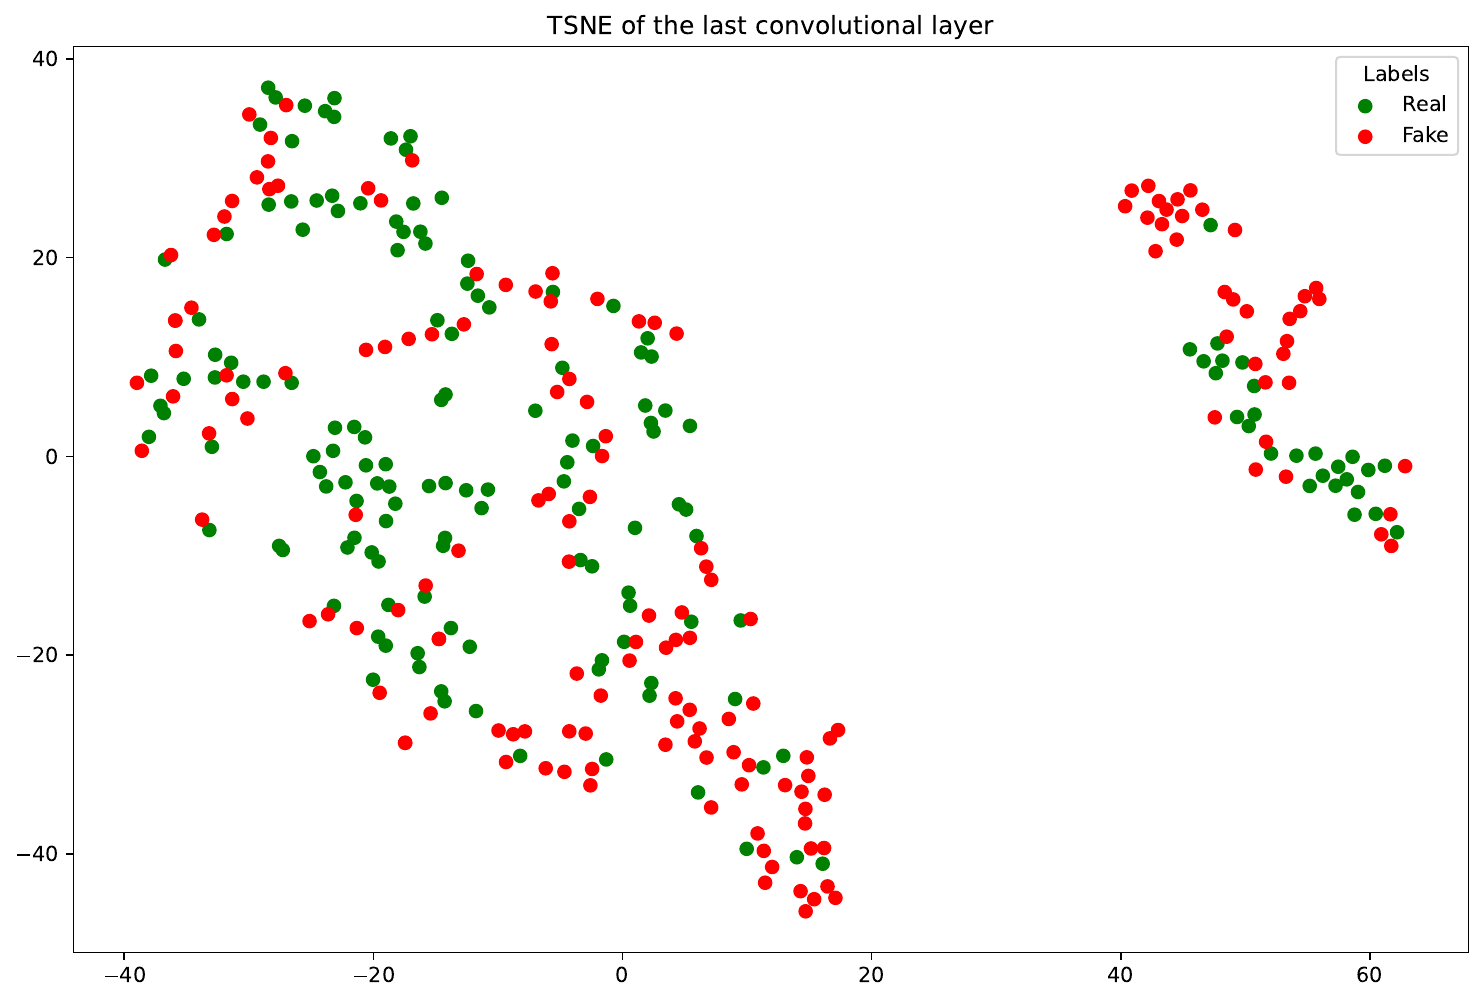
\includegraphics[width=0.45\textwidth]{TSNE_GraphSAGE_POL.png}\label{subfig:TSNE_GraphSAGE_POL}}
    \caption[t-SNE visualizations for GraphSAGE.]{t-SNE visualizations for max pooled GraphSAGE outputs on UPFD datasets.}
    \label{fig:TSNE_GraphSAGE}
\end{figure}
Clearly, GraphSAGE is able to distinguish fake and real news instances better for the UPFD-Gossipcop dataset, but it fails to make this discrimination for the UPFD-Politifact dataset. This can be due to the low amounts of instances in the UPFD-Politifact dataset.\\
\textbf{Initial Improvement Suggestions for GNNExplainer.} During our experiments, we realized that some explanations are hard to read, particularly, the ones with too many nodes and edges. Including the explanation provided in Fig.~\ref{fig:POL_RealNewsExample1Explanation_no_threshold}, it is hard to distinguish edges. In order to understand the importance of edges and simplify the explaining subgraph, we employed three simple techniques that use a threshold value. We apply this threshold value to the edge mask. This operation  sets the values less than or equal to the threshold to zero, effectively removing the corresponding edges from the explaining subgraph. The first approach is straightforward, take the maximum and the minimum value of the edge mask values. Then, set the threshold to a value less than the maximum but higher than the minimum by manual estimation, and observe the changes in the explaining subgraph as we decrease or increase the threshold value. This approach is too much manual work, so we came up with a more systematic approach. The second approach is to get the mean of all edge mask values for the current instance to get a threshold value. This way, we obtain fewer edges in our initial explanation but keep an important set of edges to understand their importance. Our third approach is to take the median of the edge mask set as a threshold. There were no big differences between the mean and median methods. However, we opted for the median method as it was able to capture more edges for small explaining subgraphs compared to the mean method. We illustrate the effect of the threshold methods on a real news instance from the UPFD-Politifact dataset in Fig~\ref{fig:POL_RealNewsExample2Explanation_with_threshold}.\\
\begin{figure}
    \centering
    \subfloat[Second real news instance from UPFD-Politifact.]{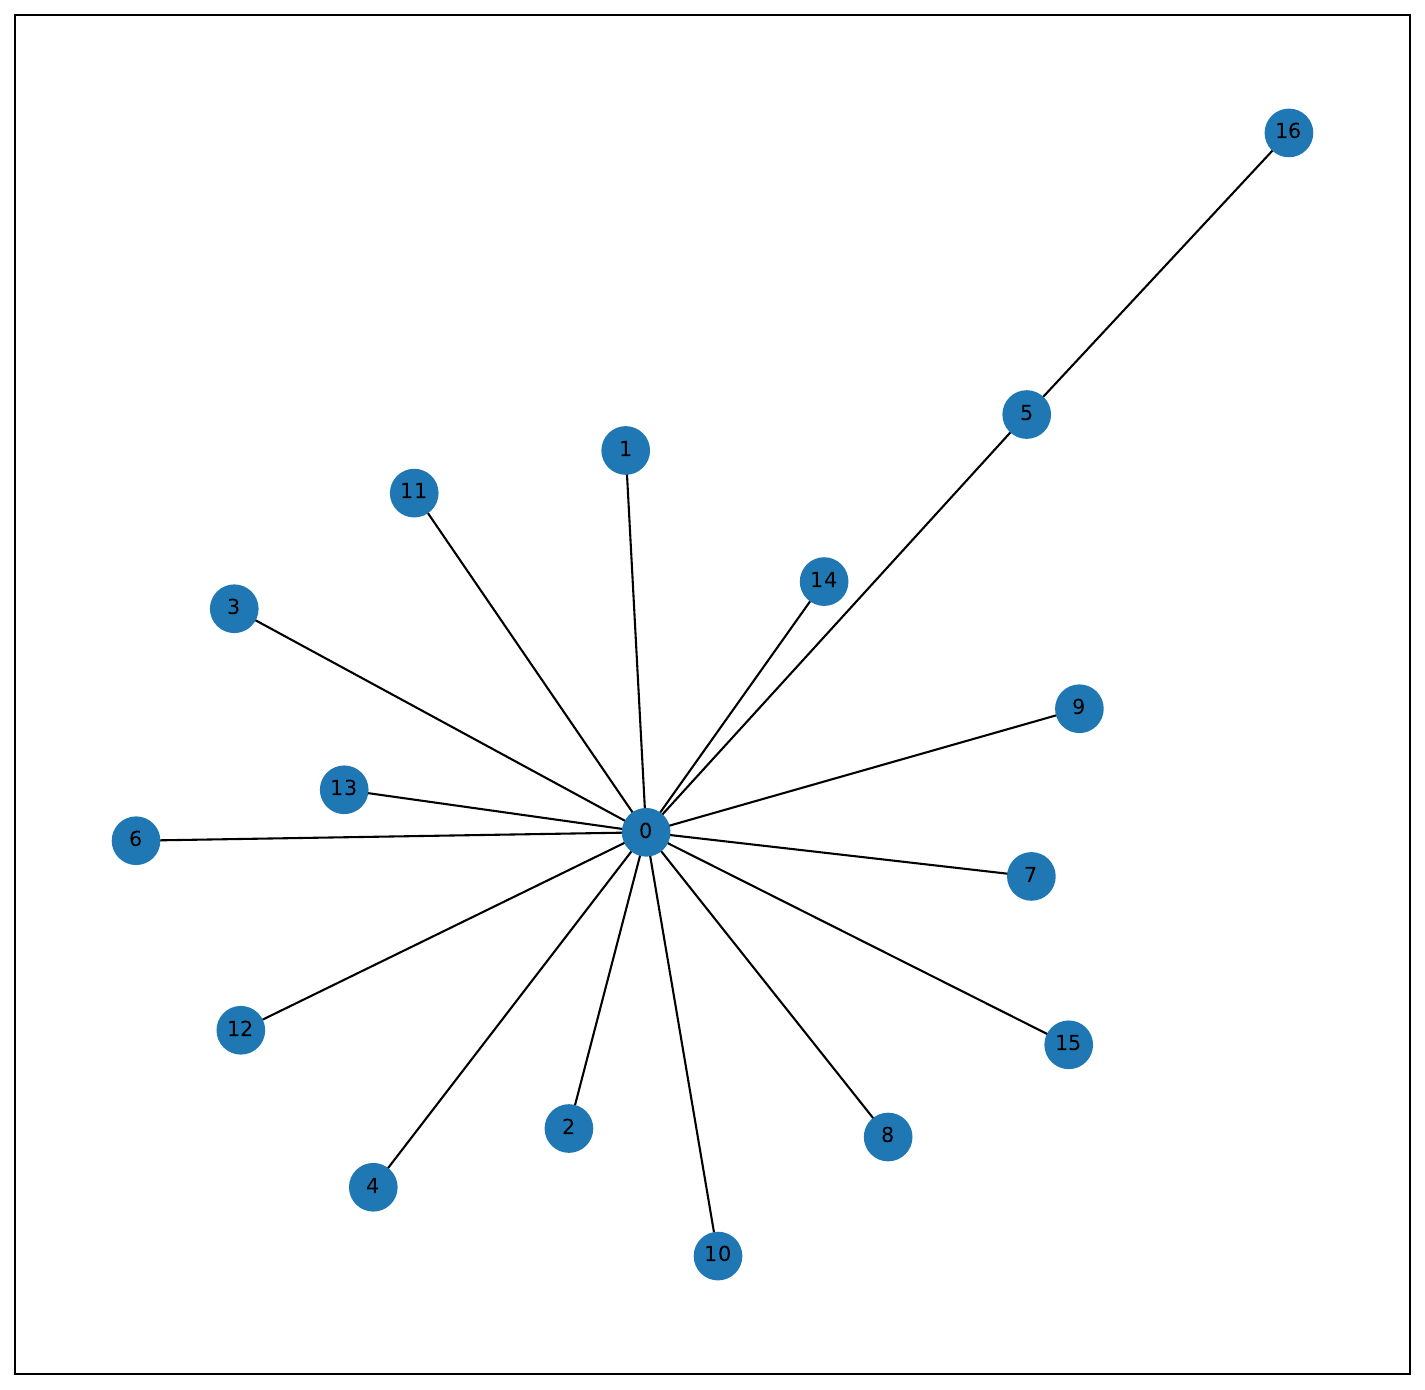
\includegraphics[width=0.45\textwidth]{POL_RealNewsExample2.png}}
    \hfill
    \subfloat[The explaining subgraph provided for the second real news instance.]{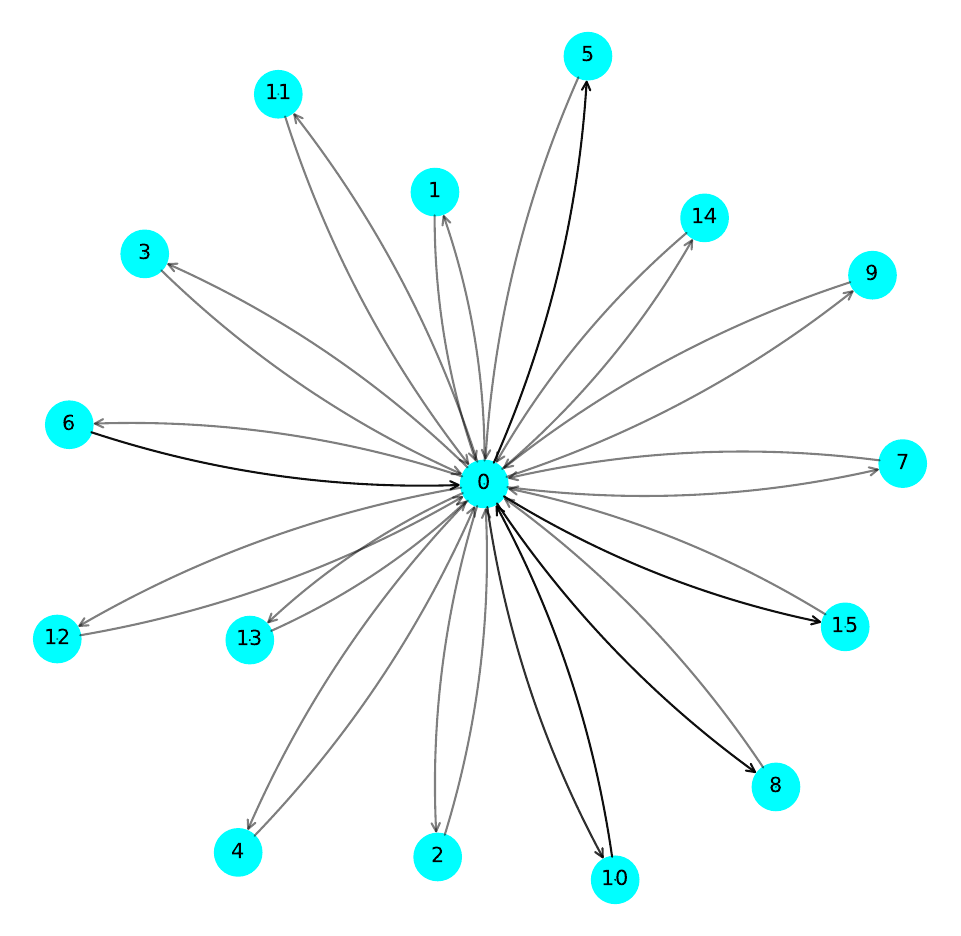
\includegraphics[width=0.45\textwidth]{POL_RealNewsExample2Explanation_no_threshold.png}}
    \hfill
    \subfloat[The explaining subgraph with median method applied.]{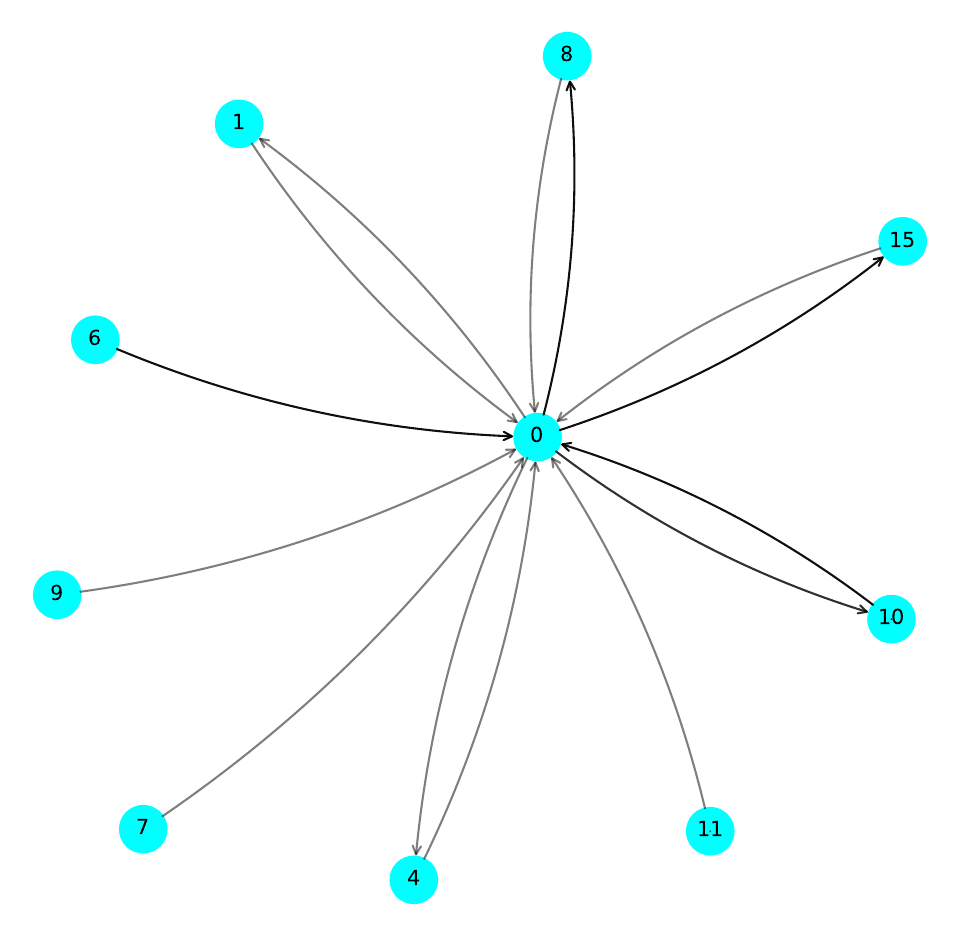
\includegraphics[width=0.45\textwidth]{POL_RealNewsExample2Explanation_with_threshold_median.png}}
    \hfill
    \subfloat[The explaining subgraph with mean method applied.]{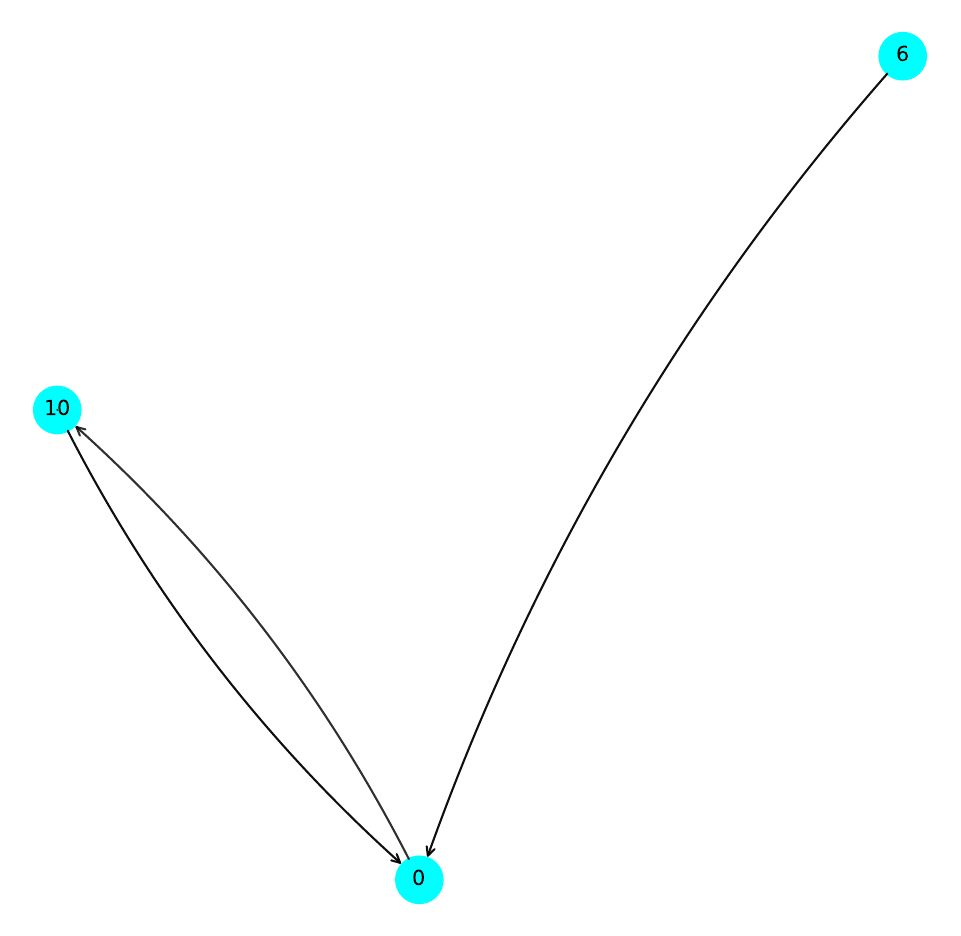
\includegraphics[width=0.45\textwidth]{POL_RealNewsExample2Explanation_with_threshold_mean.png}}
    \caption[Outputs of threshold methods for the explaining subgraph of the second real news example from UPFD-Politifact.]{Outputs of threshold methods for the explaining subgraph of the second real news example from UPFD-Politifact. We can observe that the median method provides more edges than the mean method for a relatively small explaining subgraph. Also, we can observe the importance of edges visually in the explanations. Some edges are more opaque than the other ones, this indicates that these edges are more important than the more transparent ones.}
    \label{fig:POL_RealNewsExample2Explanation_with_threshold}
\end{figure}
We can extend our method to an interactive plot in which we are able to change the threshold value dynamically. Furthermore, we can use the edge mask values provided for the edges in the subgraph to apply average and mean thresholding methods. We leave this for future work.\\
\textbf{Introducing Unseen Data.} We randomly sampled one fake news instance from the UPFD-Gossipcop dataset, which is unseen data for the UPFD classifier that was trained on the UPFD-Politifact dataset. We did not generate a new graph instance as obtaining the news piece, creating embeddings for it, and collecting its social context information is a cumbersome process without this data prepared beforehand.\\
\begin{figure}
    \centering
    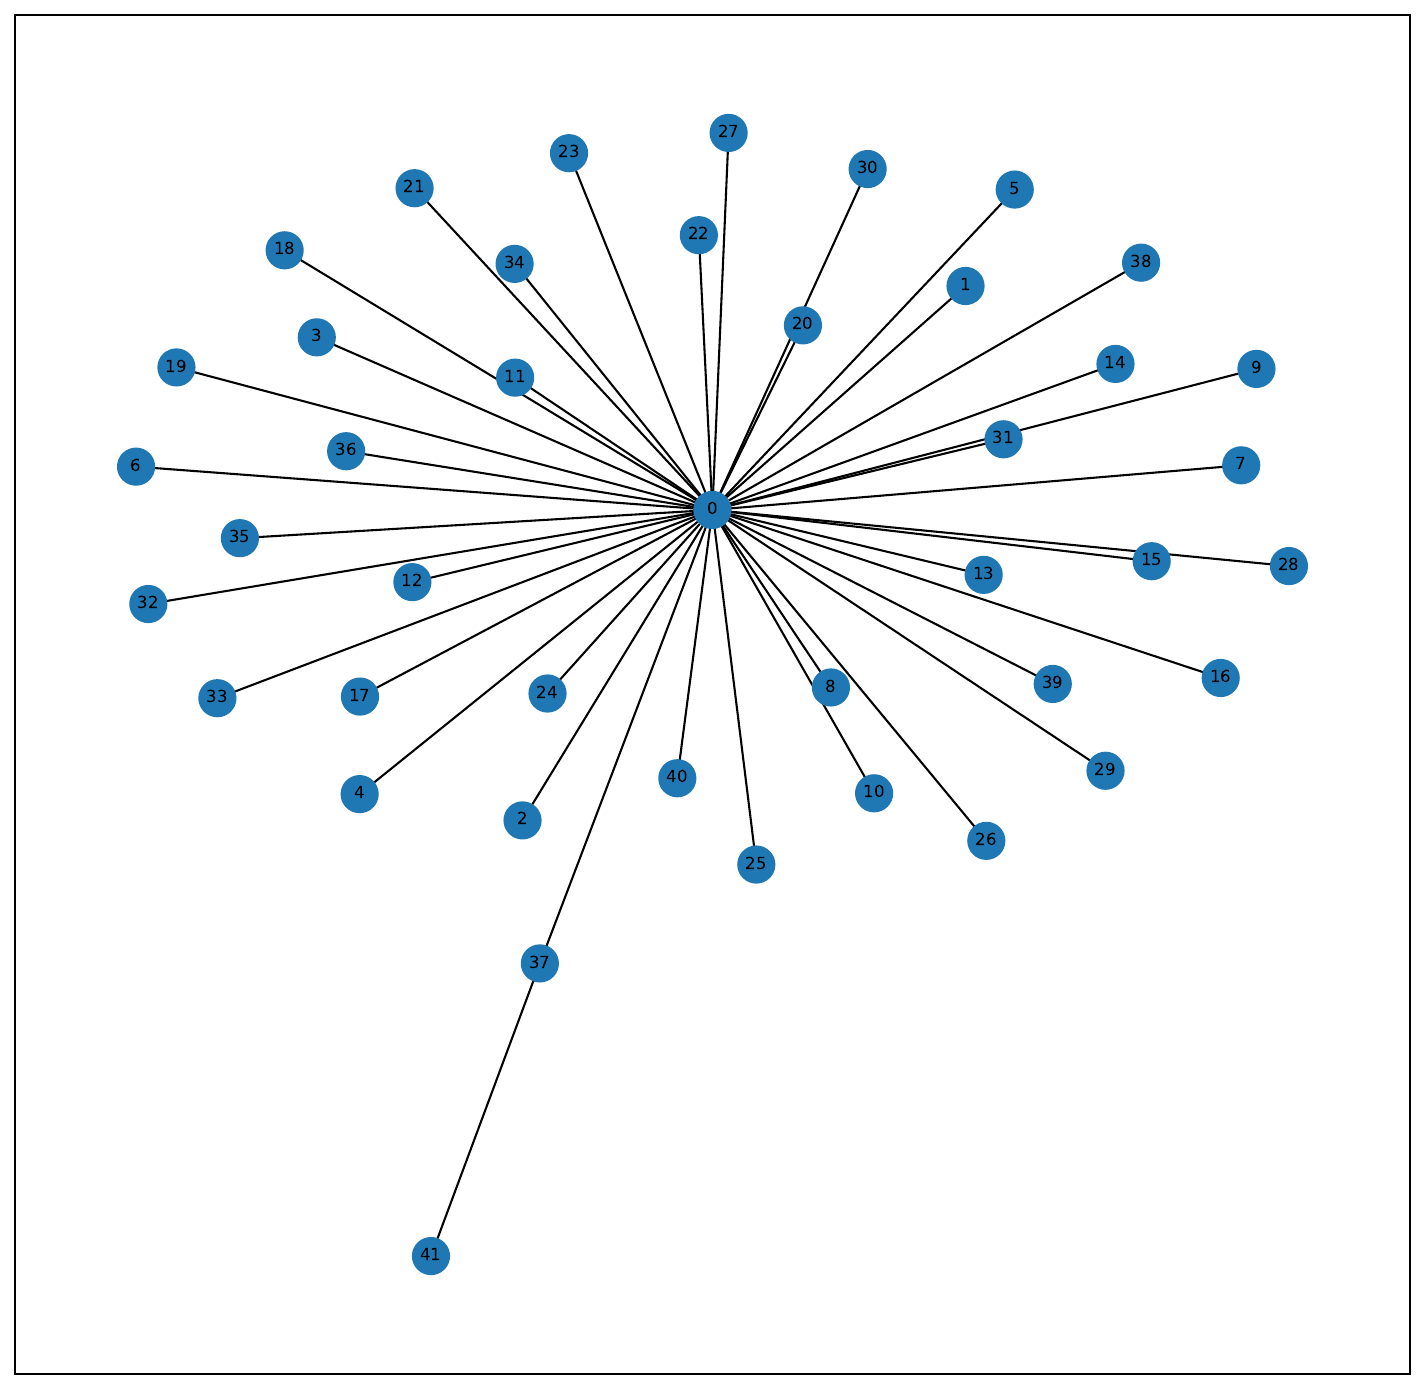
\includegraphics[scale=0.45]{GOS_FakeNewsExample1}
    \caption[A fake news example from UPFD-Gossipcop.]{A fake news example from UPFD-Gossipcop. We introduced this instance as an unseen data to the UPFD classifier, and it predicted this fake news piece as real with a probability of 0.9984.}
    \label{fig:GOS_FakeNewsExample1}
\end{figure}
Our unseen fake news example from the UPFD-Gossipcop dataset is illustrated in Fig.~\ref{fig:GOS_FakeNewsExample1}. We observe that this fake news piece does not display echo chamber patterns. In fact, structurally, it looks more like a real news piece from the UPFD-Politifact dataset. This may be why the UPFD classifier mispredicted this instance. Let us dive further into understanding this. There can be a variety of reasons. It can be because of the difference in the news style in both datasets. The UPFD-Politifact dataset houses a set of political news, whereas the UPFD-Gossipcop dataset houses a massive set of celebrity news. So, the difference in textual content could be a reason. Another reason can be the small number of training instances for the UPFD-Politifact dataset. However, we were not able to gather suggestive information from the explanation. Therefore, we did not include it. One way to understand whether the UPFD classifier responds to echo chamber structures is to create these echo chambers by adding children nodes to some of the cascade nodes and feeding this to the UPFD classifier. To test this, we added 20 nodes with no information in them and selected nodes $v_{37}$ and $v_{39}$ arbitrarily to be the spreaders. The resulting graph is illustrated in Fig.~\ref{fig:GOS_FakeNewsExample1Perturbed}.
\begin{figure}
    \centering
    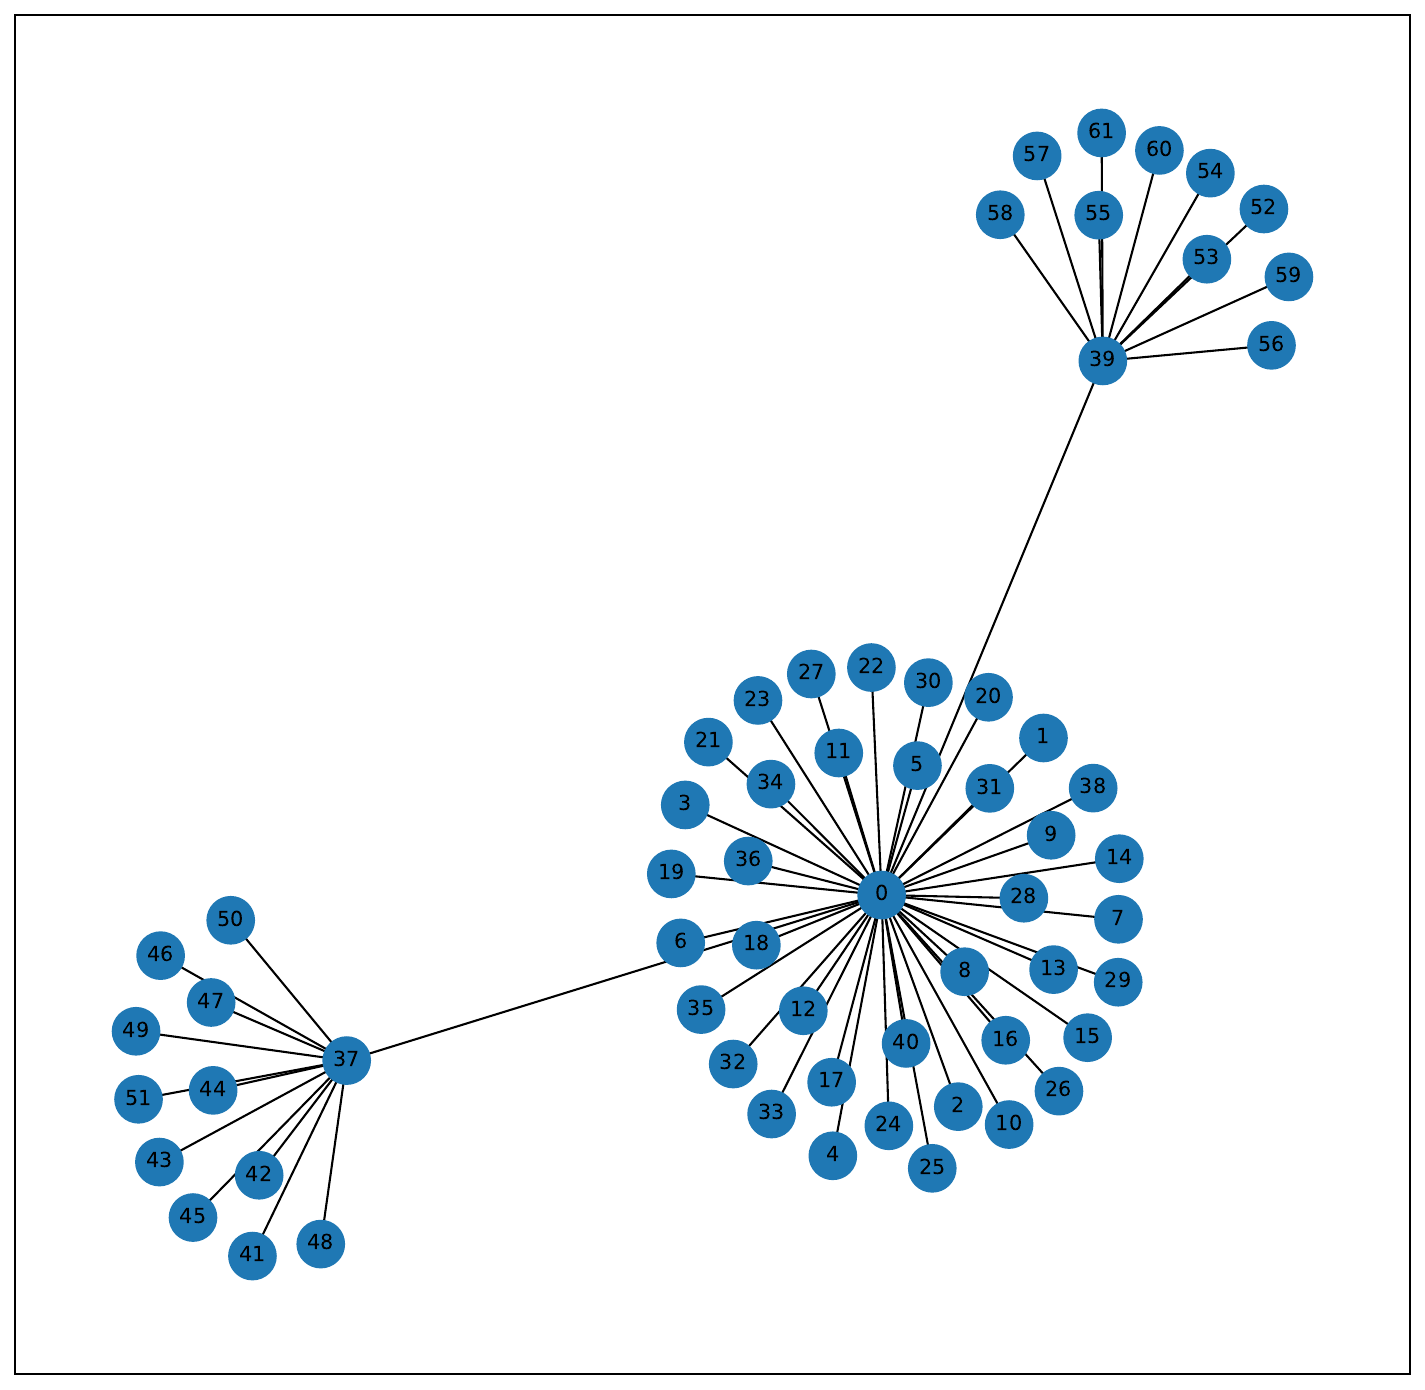
\includegraphics[scale=0.45]{GOS_FakeNewsExample1Perturbed}
    \caption[The perturbed version of the fake news example from the UPFD-Gossipcop dataset.]{The perturbed version of the fake news example from the UPFD-Gossipcop dataset. We added echo-chamber like structures to nodes $v_{37}$ and $v_{39}$.}
    \label{fig:GOS_FakeNewsExample1Perturbed}
\end{figure}
When the fed the perturbed sample to the UPFD classifier, the prediction probability of the label "fake" slightly increased. So we also sampled some historical information from a randomly obtained fake news instance that is different from the one we are analyzing. We embedded the new nodes with randomly obtained users' historical information. Then we fed this instance to the UPFD classifier, but the change in probability was too small that it could be omitted. Thus, for this instance, our experiment suggests that the existence of echo chamber structures does not increase the probability of the prediction of fake news.\\
% maybe include real news example from Gossipcop here.
\textbf{Target Audience, XAI Goals, and Final Improvement Suggestions.} Understanding the UPFD classifier's behavior locally with just a visualization is not sufficient for an end user to understand why a particular news piece was predicted as real or fake. However, given enough resources, one can reverse engineer the process in the UPFD framework, which would allow for the analysis of the node feature masks of the news content and historical information embeddings. That would increase the transparency and informativeness of the UPFD classifier. We also suggest employing interactive visualizations when working with GNNExplainer since the explanations can get very complex. Explanations produced by GNNExplainer should be investigated by a data scientist who will simplify the explanation for a domain expert or an end user. For UPFD, this simplification process can include aggregation of bidirectional edge mask values so that they can be represented as an undirected edge. Moreover, these undirected edges can be color-coded such that each color represents a value above a certain threshold which can be obtained using the methods we suggested. For example, for a big explaining subgraph, we can group the edge masks using predefined number of categories, each of which is represented by a color, then display the edges with those colors in the explaining subgraph. Also, for GNNs with language models, the node features should be easily mappable to the textual content in such a way that we can create a variation of force plots provided by the SHAP framework.\\
To sum up, we have analyzed the explanations produced by GNNExplainer for the UPFD classifier, which was trained on the UPFD-Politifact dataset. We have observed some of the statistically significant features' existence in the explanations. We have also stressed the shortcomings of GNNExplainer and suggested simple yet effective methods to reduce the complexity of an explanation. All experiments were conducted using Python 3.7~\parencite{Python_Rossum}, PyTorch 1.11.0~\parencite{PyTorch_Paszke}, and PyTorch Geometric 2.0.4~\parencite{PyTorchGeometric_Fey}. All visualizations were obtained through the use of NetworkX 2.6.3~\parencite{NetworkX_Hagberg}, and Matplotlib 3.5.1~\parencite{Matplotlib_Hunter}. The detailed library usage and the implementation of all models are provided in our GitHub repository~\footnote{\url{https://github.com/sersery35/Explainability_of_FND_Models/tree/main/GNNFakeNews}}.
% !TeX root = ../main.tex
% Add the above to each chapter to make compiling the PDF easier in some editors.

\chapter{Conclusion}\label{chapter:conclusion}
Automated FND is becoming a necessity as more people obtain their news from social media or the web. While the source of a news piece is vital for its authenticity, history observed that even the most trustworthy sources could share fake news. The dissemination of fake news leads to more misinformed people, creating a worldwide issue. Many researchers have tried to build FND systems in various settings to tackle this problem. With the evolution of ML systems, FND systems became automated. Nevertheless, automated FND is still challenging due to the ever-changing format of fake news, malicious accounts, outdated or missing datasets, and the lack of reproducible code. The research community should put in more effort to tackle the issue of fake news.\\
Moreover, all the FND works we have observed reported their performance for their model, but they did not attempt to utilize explanation methods to interpret the model's behavior. To our best knowledge, this is the first work that attempts to explain FND models. We strongly encourage the researchers to adopt explanation methods for their models to understand their models' behavior. As we observed in~\ref{subsec:ExplainingNewsContentModels_ExplainingNewsContentClassifier}, we could trick the model into predicting a fake news instance as real even though the model has seen that fake news instance in training. Adversarial examples, explanation methods, and input sensitivity analysis should be incorporated into the model development process to ensure that the model will function as intended. Particularly for black-box models like DNNs or GNNs, previously stated procedures are essential. Otherwise, one cannot completely understand whether the model has learned the actual task.\\
We listed our research objectives in Chapter~\ref{chapter:introduction}, and now, we show that we have fulfilled all of them. The first, \textbf{RO1}, is satisfied in Chapter~\ref{chapter:background}, in which we discussed explanation methods for DNNs and GNNs. We provided the intuition behind the most popular explanation methods available for FND. For all models that are not graph-based, we can easily use tools from the SHAP framework; for GNNs, we utilize GNNExplainer. \\
For the second objective, we have shown that a model can be deceived with several perturbations to the input. So we adopted the partition explainer to help us uncover this fallacy. We showed that this fallacy was closely related to the  model's architecture and the contents of the dataset. We then retrained the news content model so that we could analyze it without the features that were causing the issue. We obtained a similar performance with better base values, which suggests that the model learned to distinguish between the news by looking at more complex features. Thus, \textbf{RO2} is fulfilled in~\ref{subsec:ExplainingNewsContentModels_ExplainingNewsContentClassifier}.\\
For the last objective, \textbf{RO3}, our suggestions are twofold. The first is for the explanations from the partition explainer. We suggested the usage of bar plots of Owen values for long texts in~\ref{subsec:ExplainingNewsContentModels_ExplainingNewsContentClassifier}. The second is for the explanations from GNNExplainer. We proposed in~\ref{subsec:ExplaniningGNNs_ExplainingUPFDClassifier} to use median or mean for edge masks where the explanation is too complex. We discuss the understandability and structure of explanations regarding the input data. We recommend producing explanations in the same form as the input, which would increase the understandability of the explanations. Although, this is a complicated task considering GNNExplainer attempts to explain all non-euclidean data, thus providing an explanation for every type. For this shortcoming for tree-structured datasets, we suggest aggregating the edge mask values of the edges between the same nodes so that the explanation will resemble the input. Furthermore, we suggest the adoption of interactive plots for GNNExplainer so that one can observe the changes in edges and nodes as they interact with the threshold.\\
In addition to the research objectives, we showed that utilizing social context data with news content data can increase performance by sensitivity analysis. We also discussed how to interpret explanations from GNNExplainer, analyzed its explanations' faithfulness, and observed the news content's importance for a prediction done by a GNN model. We stressed in~\ref{subsec:ExplaniningGNNs_ExplainingUPFDClassifier} the importance of the availability of the news content in UPFD to utilize node feature masks, which can then be illustrated with the text input similar to the way the SHAP framework does. Thus, we could not analyze the importance per token in a news piece because of the limitations we enumerated in~\ref{subsec:ExplaniningGNNs_ExplainingUPFDClassifier}.\\
Furthermore, incompatibility issues of DeepSHAP with Transformer models, outdated datasets, and the availability of the datasets were other limitations. For instance, our attempt to construct FakeNewsNet from the authors' code took more than two months to download only around 80\% of the dataset. Therefore, we were not able to analyze the UPFD classifier's behavior in depth. Fortunately, the incompatibility issue of DeepSHAP was mitigated by the model-agnostic partition explainer.\\
The research community took a particular interest in FND, and new studies are considering these limitations in their designs. Lately, the discussion of model aging and early fake news detection has gained momentum. As we discussed in ~\ref{subsec:fakeNewsDetection_fakeNews}, fake news tends to spread too fast. Hence, a model that can detect fake news pieces before they reach their peak dissemination is necessary. Otherwise, due to the psychologica tendencies of humans, we will not be able to alleviate the adverse effects of fake news. The ever-changing nature of fake news content gives rise to the necessity of FND systems with continual learning, which~\citeauthor{GraphNeuralNetworksWithContinualLearningFakeNewsDetection_Han} (\citeyear{GraphNeuralNetworksWithContinualLearningFakeNewsDetection_Han}) discuss. We encourage a similar approach for FND to create robust automated systems.\\
Undertaking these limitations should be the next step in future research. Without well-structured and informative datasets, developing a competitive model is not possible. Specifically, rich datasets like UPFD should provide more information about their process so that more insight can be gained from the dataset and explanations. Therefore, as a final word, we draw attention to the importance of the availability of datasets and reproducible studies and urge researchers to be more contributing on this matter.
% TODO: add more chapters here

\appendix{}

\microtypesetup{protrusion=false}
\listoffigures{}
\listoftables{}
\microtypesetup{protrusion=true}
\printbibliography{}

\end{document}
